\documentclass[aps,preprint,preprintnumbers,nofootinbib,showpacs,prd]{revtex4-1}
\usepackage{graphicx,color}
\usepackage{caption}
\usepackage{subcaption}
\usepackage{amsmath,amssymb}
\usepackage{multirow}
\usepackage{amsthm}%        But you can't use \usewithpatch for several packages as in this line. The search 

\usepackage{cancel}

%%% for SLE
\usepackage{dcolumn}   % needed for some tables
\usepackage{bm}        % for math
\usepackage{amssymb}   % for math
\usepackage{multirow}
%%% for SLE -End

\usepackage{ulem}
\usepackage{cancel}

\usepackage{hyperref}

\usepackage[top=1in, bottom=1.25in, left=1.1in, right=1.1in]{geometry}

\usepackage{mathtools} % for \DeclarePairedDelimiter{\ceil}{\lceil}{\rceil}

\usepackage{simplewick}

\newcommand{\msout}[1]{\text{\sout{\ensuremath{#1}}}}


%%%%%% My stuffs - Stef
\newcommand{\lsim}{\mathrel{\mathop{\kern 0pt \rlap
  {\raise.2ex\hbox{$<$}}}
  \lower.9ex\hbox{\kern-.190em $\sim$}}}
\newcommand{\gsim}{\mathrel{\mathop{\kern 0pt \rlap
  {\raise.2ex\hbox{$>$}}}
  \lower.9ex\hbox{\kern-.190em $\sim$}}}

%
% Key
%
\newcommand{\key}[1]{\medskip{\sffamily\bfseries\color{blue}#1}\par\medskip}
%\newcommand{\key}[1]{}
\newcommand{\q}[1] {\medskip{\sffamily\bfseries\color{red}#1}\par\medskip}
\newcommand{\comment}[2]{{\color{red}{{\bf #1:}  #2}}}


\newcommand{\ie}{{\it i.e.} }
\newcommand{\eg}{{\it e.g.} }

%
% Energy scales
%
\newcommand{\ev}{{\,{\rm eV}}}
\newcommand{\kev}{{\,{\rm keV}}}
\newcommand{\mev}{{\,{\rm MeV}}}
\newcommand{\gev}{{\,{\rm GeV}}}
\newcommand{\tev}{{\,{\rm TeV}}}
\newcommand{\fb}{{\,{\rm fb}}}
\newcommand{\ifb}{{\,{\rm fb}^{-1}}}

%
% SUSY notations
%
\newcommand{\neu}{\tilde{\chi}^0}
\newcommand{\neuo}{{\tilde{\chi}^0_1}}
\newcommand{\neut}{{\tilde{\chi}^0_2}}
\newcommand{\cha}{{\tilde{\chi}^\pm}}
\newcommand{\chao}{{\tilde{\chi}^\pm_1}}
\newcommand{\chaop}{{\tilde{\chi}^+_1}}
\newcommand{\chaom}{{\tilde{\chi}^-_1}}
\newcommand{\Wpm}{W^\pm}
\newcommand{\chat}{{\tilde{\chi}^\pm_2}}
\newcommand{\smu}{{\tilde{\mu}}}
\newcommand{\smur}{\tilde{\mu}_R}
\newcommand{\smul}{\tilde{\mu}_L}
\newcommand{\sel}{{\tilde{e}}}
\newcommand{\selr}{\tilde{e}_R}
\newcommand{\sell}{\tilde{e}_L}
\newcommand{\smurl}{\tilde{\mu}_{R,L}}

\newcommand{\casea}{\texttt{IA}}
\newcommand{\caseb}{\texttt{IB}}
\newcommand{\casec}{\texttt{II}}

\newcommand{\caseasix}{\texttt{IA-6}}

%
% Greek
%
\newcommand{\es}{{\epsilon}}
\newcommand{\sg}{{\sigma}}
\newcommand{\dt}{{\delta}}
\newcommand{\kp}{{\kappa}}
\newcommand{\lm}{{\lambda}}
\newcommand{\Lm}{{\Lambda}}
\newcommand{\gm}{{\gamma}}
\newcommand{\mn}{{\mu\nu}}
\newcommand{\Gm}{{\Gamma}}
\newcommand{\tho}{{\theta_1}}
\newcommand{\tht}{{\theta_2}}
\newcommand{\lmo}{{\lambda_1}}
\newcommand{\lmt}{{\lambda_2}}
%
% LaTeX equations
%
\newcommand{\beq}{\begin{equation}}
\newcommand{\eeq}{\end{equation}}
\newcommand{\bea}{\begin{eqnarray}}
\newcommand{\eea}{\end{eqnarray}}
\newcommand{\ba}{\begin{array}}
\newcommand{\ea}{\end{array}}
\newcommand{\bit}{\begin{itemize}}
\newcommand{\eit}{\end{itemize}}

\newcommand{\nbea}{\begin{eqnarray*}}
\newcommand{\neea}{\end{eqnarray*}}
\newcommand{\nbeq}{\begin{equation*}}
\newcommand{\neeq}{\end{equation*}}

\newcommand{\no}{{\nonumber}}
\newcommand{\td}[1]{{\widetilde{#1}}}
\newcommand{\sqt}{{\sqrt{2}}}
%
\newcommand{\me}{{\rlap/\!E}}
\newcommand{\met}{{\rlap/\!E_T}}
\newcommand{\rdmu}{{\partial^\mu}}
\newcommand{\gmm}{{\gamma^\mu}}
\newcommand{\gmb}{{\gamma^\beta}}
\newcommand{\gma}{{\gamma^\alpha}}
\newcommand{\gmn}{{\gamma^\nu}}
\newcommand{\gmf}{{\gamma^5}}
%
% Roman expressions
%
\newcommand{\br}{{\rm Br}}
\newcommand{\sign}{{\rm sign}}
\newcommand{\Lg}{{\mathcal{L}}}
\newcommand{\M}{{\mathcal{M}}}
\newcommand{\tr}{{\rm Tr}}

\newcommand{\msq}{{\overline{|\mathcal{M}|^2}}}

%
% kinematic variables
%
%\newcommand{\mc}{m^{\rm cusp}}
%\newcommand{\mmax}{m^{\rm max}}
%\newcommand{\mmin}{m^{\rm min}}
%\newcommand{\mll}{m_{\ell\ell}}
%\newcommand{\mllc}{m^{\rm cusp}_{\ell\ell}}
%\newcommand{\mllmax}{m^{\rm max}_{\ell\ell}}
%\newcommand{\mllmin}{m^{\rm min}_{\ell\ell}}
%\newcommand{\elmax} {E_\ell^{\rm max}}
%\newcommand{\elmin} {E_\ell^{\rm min}}
\newcommand{\mxx}{m_{\chi\chi}}
\newcommand{\mrec}{m_{\rm rec}}
\newcommand{\mrecmin}{m_{\rm rec}^{\rm min}}
\newcommand{\mrecc}{m_{\rm rec}^{\rm cusp}}
\newcommand{\mrecmax}{m_{\rm rec}^{\rm max}}
%\newcommand{\mpt}{\rlap/p_T}

%%%song
\newcommand{\cosmax}{|\cos\Theta|_{\rm max} }
\newcommand{\maa}{m_{aa}}
\newcommand{\maac}{m^{\rm cusp}_{aa}}
\newcommand{\maamax}{m^{\rm max}_{aa}}
\newcommand{\maamin}{m^{\rm min}_{aa}}
\newcommand{\eamax} {E_a^{\rm max}}
\newcommand{\eamin} {E_a^{\rm min}}
\newcommand{\eaamax} {E_{aa}^{\rm max}}
\newcommand{\eaacusp} {E_{aa}^{\rm cusp}}
\newcommand{\eaamin} {E_{aa}^{\rm min}}
\newcommand{\exxmax} {E_{\neuo \neuo}^{\rm max}}
\newcommand{\exxcusp} {E_{\neuo \neuo}^{\rm cusp}}
\newcommand{\exxmin} {E_{\neuo \neuo}^{\rm min}}
%\newcommand{\mxx}{m_{XX}}
%\newcommand{\mrec}{m_{\rm rec}}
\newcommand{\erec}{E_{\rm rec}}
%\newcommand{\mrecmin}{m_{\rm rec}^{\rm min}}
%\newcommand{\mrecc}{m_{\rm rec}^{\rm cusp}}
%\newcommand{\mrecmax}{m_{\rm rec}^{\rm max}}
%%%song

\newcommand{\mc}{m^{\rm cusp}}
\newcommand{\mmax}{m^{\rm max}}
\newcommand{\mmin}{m^{\rm min}}
\newcommand{\mll}{m_{\mu\mu}}
\newcommand{\mllc}{m^{\rm cusp}_{\mu\mu}}
\newcommand{\mllmax}{m^{\rm max}_{\mu\mu}}
\newcommand{\mllmin}{m^{\rm min}_{\mu\mu}}
\newcommand{\mllcusp}{m^{\rm cusp}_{\mu\mu}}
\newcommand{\elmax} {E_\mu^{\rm max}}
\newcommand{\elmin} {E_\mu^{\rm min}}
\newcommand{\elmaxw} {E_W^{\rm max}}
\newcommand{\elminw} {E_W^{\rm min}}
\newcommand{\R} {{\cal R}}

\newcommand{\ewmax} {E_W^{\rm max}}
\newcommand{\ewmin} {E_W^{\rm min}}
\newcommand{\mwrec}{m_{WW}}
\newcommand{\mwrecmin}{m_{WW}^{\rm min}}
\newcommand{\mwrecc}{m_{WW}^{\rm cusp}}
\newcommand{\mwrecmax}{m_{WW}^{\rm max}}

\newcommand{\mpt}{{\rlap/p}_T}

%%%%%% END My stuffs - Stef

\newcommand{\dunno}{$ {}^{\mbox {--}}\backslash(^{\rm o}{}\underline{\hspace{0.2cm}}{\rm o})/^{\mbox {--}}$}

\DeclarePairedDelimiter{\ceil}{\lceil}{\rceil}
\DeclarePairedDelimiter{\floor}{\lfloor}{\rfloor}

\DeclareMathOperator{\ord}{ord}
\DeclareMathOperator{\tor}{tor}





\begin{document}

\title{Apostol's Analytic Number Theory}
\bigskip
\author{Stefanus$^1$\\
$^1$ Samsung Semiconductor Inc\\ San Jose, CA 95134 USA\\
}
%
\date{\today}
%
\begin{abstract}
Just for fun :)

\end{abstract}
%
\maketitle

\renewcommand{\theequation}{A.\arabic{equation}}  % redefine the command that creates the equation no.
\setcounter{equation}{0}  % reset counter 

\bigskip
\underline{\textbf{\textit{Chapter 1}}}
\bigskip

{\bf Problem 1.11}. Prove that $n^4 + 4$ is composite if $n > 1$.

This problem can be easily solved by completing the square
%
\nbea
n^4 + 4 & = & (n^2)^2 + 2^2 \\
& = & (n^2 + 2)^2 - (2n)^2 \\
& = & (n^2 + 2 - 2n)(n^2 + 2 + 2n)
\neea
%
But, suppose you're not aware of completing the square trick, here's what you can do. Since $4$ is even if $n$ is also even then $n^4 + 4$ is guaranteed to be composite. What if $n$ is odd? Let's see
%
\nbea
\begin{array}{r c r c r c r}
3^4 + 4 & = & 8\underline{1} &+& 4 &=& 8\underline{5} \\
5^4 + 4 & = & 62\underline{5} &+& 4 &=& 62\underline{9} \\
7^4 + 4 & = & 240\underline{1} &+& 4 &=& 240\underline{5} \\
9^4 + 4 & = & 656\underline{1} &+& 4 &=& 656\underline{5} \\
11^4 + 4 & = & 1464\underline{1} &+& 4 &=& 1464\underline{5} \\
13^4 + 4 & = & 2856\underline{1} &+& 4 &=& 2856\underline{5} \\
15^4 + 4 & = & 5062\underline{5} &+& 4 &=& 5062\underline{9}
\end{array}
\neea
%
so we see that if $n \not\equiv 0 \pmod{5}$ then $n^4 \equiv 1 \pmod{10}$ and therefore $n^4 + 4 \equiv 0 \pmod{5}$ and if $n \equiv 0 \pmod{5}$ then $n^4 + 4 \equiv -1 \pmod{5}$, does this always apply? well, let's do everything in mod 5 then
%
\nbea
\begin{array}{r c l c r c l}
n & \equiv & 1\pmod{5} & \to & 1^4 + 4 & \equiv & 0 \pmod {5} \\
n & \equiv & 2\pmod{5} & \to & 2^4 + 4 & \equiv & 0 \pmod {5} \\
n & \equiv & 3\pmod{5} & \to & 3^4 + 4 & \equiv & 0 \pmod {5} \\
n & \equiv & 4\pmod{5} & \to & 4^4 + 4 & \equiv & 0 \pmod {5} \\
n & \equiv & 5\pmod{5} & \to & 5^4 + 4 & \equiv & 4 \pmod {5}
\end{array}
\neea
%
So it is true, for $n \not\equiv 0 \pmod{5}$, $n^4 + 4 \equiv 0 \pmod{5}$ and thus $5|n^4 + 4$ and $n^4 + 4$ is composite, except for $n=1$ of course where $1^4 + 4 = 5$ which is prime.

Our task is to now see if we can prove that $n^4 + 4 \equiv 4 \pmod{5}$ is composite. We know that if $n$ is even then we are done, our task now is to see what happens if $n$ is odd and a multiple of $5$, \ie to check whether $(5(2k+1))^4 + 4$ is composite.

A strategy would be to show explicitly that we can factorize $(5(2k+1))^4 + 4 = (5a + 2)(5b + 2)$. The way I did it was to try out different $k$'s and see if there's a pattern to $a$ and $b$
%
\nbea
\begin{array}{r c l c r c l r c l c r c l r c l}
k &=& 0 & ~\to~ & a &=& 3 &,~b&=&7 &~~~& \frac{a}{2k+1} &=& \underline{0}3 &,~b-a &=& 4  + 8\cdot \underline{0}\\
k &=& 1 & ~\to~ & a &=& 39 &,~b&=&51 &~~~& \frac{a}{2k+1} &=& \underline{1}3 &,~b-a &=& 4 + 8\cdot \underline{1} \\
k &=& 2 & ~\to~ & a &=& 115 &,~b&=&135 &~~~& \frac{a}{2k+1} &=& \underline{2}3 &,~b-a &=& 4  + 8\cdot \underline{2}\\
k &=& 3 & ~\to~ & a &=& 231 &,~b&=&259 &~~~& \frac{a}{2k+1} &=& \underline{3}3 &,~b-a &=& 4  + 8\cdot \underline{3}\\
k &=& 4 & ~\to~ & a &=& 387 &,~b&=&423 &~~~& \frac{a}{2k+1} &=& \underline{4}3 &,~b-a &=& 4  + 8\cdot \underline{4}\\
k &=& 5 & ~\to~ & a &=& 583 &,~b&=&627 &~~~& \frac{a}{2k+1} &=& \underline{5}3 &,~b-a &=& 4  + 8\cdot \underline{5}\\
k &=& 6 & ~\to~ & a &=& 819 &,~b&=&871 &~~~& \frac{a}{2k+1} &=& \underline{6}3 &,~b-a &=& 4  + 8\cdot \underline{6}\\
k &=& 7 & ~\to~ & a &=& 1095 &,~b&=&1155 &~~~& \frac{a}{2k+1} &=& \underline{7}3 &,~b-a &=& 4  + 8\cdot \underline{7}
\end{array}
\neea
%
so it seems like $a = (2k+1)(10k+3) = 20k^2+16k+3$ and $b = a + 4 + 8k= 20k^2+24k+7$ and indeed if we expand
%
\nbea
(5a + 2)(5b + 2) & = & (5(20k^2+16k+3) + 2)(5(20k^2+24k+7) + 2) \\
& = & 10000k^4+20000k^3+15000k^2+5000k+625 + 4 \\
& = & (5(2k+1))^4 + 4
\neea
%
so indeed $(5(2k+1))^4 + 4$ can be factorized into $(5(20k^2+16k+3) + 2)(5(20k^2+24k+7) + 2)$ therefore they must be composite.

So in short, if $n \not\equiv 0 \pmod{5}$ then $5|n^4 + 4$ and if $5|n$ then $(5(2k+1))^4 + 4 = (5(20k^2+16k+3) + 2)(5(20k^2+24k+7) + 2)$ and therefore $n^4 + 4$ is composite for $n>1$.

{\bf Problem 1.15}. Prove that every $n \ge 12$ is the sum of two composite numbers.

Here I assume the composite numbers are positive otherwise it is just a restatement of Bezout's lemma. Although this question looks tough initially it's actually very simple, for any even numbers $\ge 12$ we have
%
\nbea
2(6 + n) & = & 4 + 2(4+n)
\neea
%
with $n \ge 0$ and for any odd number $\ge 13$ we have
%
\nbea
2(6 + n) + 1 & = & 9 + 2(2 + n)
\neea
%
again with $n \ge 0$ and the reason we start with 12 is because between 1 and 12 only $8=4+4$ and $10=4+6$ are sums of composite numbers but for 12 and above, every number is a sum of composite numbers.

{\bf Problem 1.16}. Prove that if $2^n - 1$ is prime then $n$ is prime

The trick we need to know here is that
%
\nbea
x^n - 1 & = & (x - 1)(x^{n-1} + x^{n-2} + \dots + 1)
\neea
%
Thus if $n$ is not prime we must have $n = ab$
%
\nbea
2^n - 1 & = & 2^{ab} - 1 = (2^a)^b - 1 \\
\to (2^a)^b - 1 & = & (2^a - 1)((2^a)^{b-1} + (2^a)^{b-2} + \dots + 1)
\neea
%
and thus $2^n - 1$ is not prime, we can immediately generalize this to if $a^m - b^n$ is prime with $a,b > 1$ then $\gcd(m,n) = 1$ because otherwise
%
\nbea
a^m - b^n & = & a^{m'd} - b^{n'd} = (a^{m'})^d - (b^{n'})^d \\
& = & \left (a^{m'} - b^{n'} \right ) \left ((a^{m'})^{d-1} + (a^{m'})^{d-2} (b^{n'})+ \dots + (a^{m'})(b^{n'})^{d-2} + (b^{n'})^{d-1} \right )
\neea
%

{\bf Problem 1.17}. Prove that if $2^n + 1$ is prime, then $n$ is a power of 2.

The key point we need to know here is
%
\nbea
x^m + 1 & = & (x^h + 1)(x^{m-h} - x^{m-h-h} + x^{m-h-h-h} - \ldots + 1)
\neea
%
since the signs alternate from plus to minus on the RHS, the above factorization can only occur if $h|m$ and that $m/h$ is {\bf odd}. Another piece of info we need is that $(x^h-1)\nmid(x^m+1)$ for any $h$ due to the same reason and so we need not care about nor consider $x^h-1$.

Now say $n$ in the $2^n+1$ is even $\to n=2w \to 2^{2w} + 1$, now if $w$ is odd then $2^{2w} + 1$ is divisible by $2^2 + 1$, if $w$ is even we can repeat the process $w = 2t \to 2^{4t} + 1$ and again, if $t$ is odd then $2^{4t} + 1$ is divisible by $2^4 + 1$ but if $t$ is even then we again repeat the process. So the only way it is not divisible by $2^z+1$ is that the remaining factors are all even and it only happens when $n$ is a power of 2.

If $n$ is odd and composite then all factors of $n$ are odd and therefore $2^n+1$ is divisible by $2^u+1$ where $u|n$, the only case left is when $n$ is prime but in this case $2^n+1$ is immediately divisible by $2^1 + 1$ which is kind of a cool fact actually that any $2^n+1$ where $n$ is prime is divisible by 3 :)

{\bf Problem 1.18}. If $m\neq n$ compute $\gcd\left( a^{2m}+1, a^{2n}+1\right)$ in terms of $a$. [{\it Hint:} Let $A_n = a^{2n}+1$ and show that $A_n|(A_m-2)$ if $m>n$.]

Without loss of generality let's assume that $m > n$. If $d = \gcd(a^{2n}+1, a^{2m}+1)$ then $d|(a^{2m}+1) - (a^{2n}+1) \to d|a^{2n}(a^{2(m-n)} - 1)$, if $d|a^{2n}$ then since $d|(a^{2n}+1)$ this means that $d|(a^{2n}+1 - a^{2n}) \to d|1$ which is not that interesting.

The interesting part is when $d|(a^{2(m-n)} - 1)$ and since $m > n \to m = nq + r$, in this case 
%
\nbea
d &|& ((a^{2(nq+r-n)} - 1) + (a^{2n} + 1)) \\
d &|& (a^{2(n(q-1)+r)} + a^{2n}) \\
d &|& a^{2n}(a^{2(n(q-2)+r)} + 1)
\neea
%
just like before, if $d|a^{2n}$ then $d|1$, so we ignore this case, the other case is $d | (a^{2(n(q-2)+r)} + 1)$. Now, if $q-2 > 2$ we can repeat the process but this time by taking the difference
%
\nbea
d &|& ((a^{2(n(q-2)+r)} + 1) - (a^{2n} + 1)) \\
d &|& (a^{2(n(q-2)+r)} - a^{2n}) \\
d &|& a^{2n}(a^{2(n(q-3)+r)} - 1)
\neea
%
again, we can repeat the process but this time by taking the sum just like before, once we reach $n(q-q) + r = r$ (or if $q=1$ to begin with we will reach this step immediately) since $0 \le r < n$ we will now express $n = rq' + r'$ (depending on whether $q$ was even or odd we might have plus or minus in front of the constant 1 for simplicity we will choose plus)
%
\nbea
d &|& ((a^{2n} + 1) - (a^{2r} + 1)) \\
d &|& ((a^{2(rq'+r')} + 1) - (a^{2r} + 1)) \\
d &|& (a^{2(rq'+r')} - a^{2r}) \\
d &|& a^{2r'}(a^{2(r(q'-1)+r')} - 1)
\neea
%
and the process continues with the same exact pattern as Euclid's algorithm for finding the gcd between two numbers and that's what we will find, the $\gcd(m,n) = g$, \ie we will eventually get $d|(a^{2g} \pm 1)$ we can of course continue one step further to get $d|0$ (a tautology) or $d|2$ but this depends on a few things that we'll discuss later.

The next piece of information we need is the following
%
\nbea
a^{2s} - 1 & = & (a^{2r} + 1)(a^{2s-2r} - a^{2s-2r-2r} + a^{2s - 2r - 2r - 2r} -  \ldots - 1)
\neea
%
so $(a^{2r} + 1)|(a^{2s} - 1)$ if $s = rk$ where $k$ is {\it even} because we want the constant $1$ in the second bracket of the RHS to have a minus sign and the pattern of the second bracket is $+-+-+-+-\ldots$~, next,
%
\nbea
a^{2s} + 1 & = & (a^{2r} + 1)(a^{2s-2r} - a^{2s-2r-2r} + a^{2s - 2r - 2r - 2r} -  \ldots + 1)
\neea
%
by the same token $(a^{2r} + 1)|(a^{2s} + 1)$ only if $s = rk$ where $k$ is {\it odd} and last one $(a^{2r} - 1)\nmid(a^{2s} + 1)$ this is because the second bracket of the RHS must all have positive sign but the $-1$ requires a minus sign. And of course we know about
%
\nbea
a^{2s} - 1 & = & (a^{2r} - 1)(a^{2s-2r} + a^{2s-2r-2r} + a^{2s - 2r - 2r - 2r} +  \ldots + 1)
\neea
%
as long as $r|s$.

Going back to our case $d|(a^{2g}\pm1)$, first thing to note is that this means $d \le a^{2g}\pm1$. Next, let's tackle it case by case, first case, $d|(a^{2g}+1)$, we know that $d$ divides both $a^{2m}+1$ and $a^{2n}+1$ and we also know that since $m = gk_m$ and $n = gk_n$ (note that $g = \gcd(m,n)$) if $k_m$ and $k_n$ are both odd then since $d \le a^{2g} + 1$ and $(a^{2g}+1)$ divides both this means that $a^{2m}+1$ and $a^{2n}+1$, $d = a^{2g}+1$.

But if one of or both of $k_m$ or $k_n$ are even then we have something different :) Let's just assume that $k_n$ is even (this will not change the conclusion and only simplify things), now let $h = \gcd(a^{2g}+1, a^{2n}+1)$ where $n=gk_n$, this also means
%
\nbea
h &|& (a^{2n}+1) - (a^{2g}+1) \\
\to h &|& (a^{2g(k_n-1)}-1) \\
h &|& (a^{2g(k_n-2)}+1) \\
h &|& (a^{2g(k_n-3)}-1) \\
&\vdots& \\
h &|& (a^{2g(k_n-k_n)}+1) \\
\to h &|& 2
\neea
%
the last constant $1$ has a plus sign in front of it because $k_n$ is even, this means that since $d|a^{2g}+1$ and $d|a^{2n}+1$, $d \le h$ but since $h \le 2 \to d \le 2$, therefore if $a$ is odd $a^{w} + 1$ is even and $d=2$ (because $d$ is the {\it greatest} common divisor) but if $a$ is even then $a^w+1$ is odd and $d=1$.

If $d|a^{2g}-1$ then we know that from the above discussion that $(a^{2g}-1)\nmid (a^{2m} + 1), ~(a^{2g}-1)\nmid (a^{2n} + 1)$, however since $g|m,~ g|n$ the following is true $(a^{2g}-1)| (a^{2m} - 1), (a^{2g}-1)| (a^{2n} - 1)$. But this means that any common divisor $x$ between $a^{2g}-1$ and $a^{2m,n}+1$ must also divide $a^{2m,n}-1$ that is
%
\nbea
x &|& (a^{2m,n}+1) - (a^{2m,n}-1) \\
x &|& 2
\neea
%
which means that $d \le x \to d \le 2$, so again depending on whether $a$ is even or odd we get $d=1$ or $d=2$ respectively.

{\bf Problem 1.19}. The {\it Fibonacci sequence} $1,1,2,3,5,8,13,21,34,\dots$ is defined by the recursion formula $a_{n+1} = a_n + a_{n-1}$, with $a_1 = a_2 = 1$. Prove that $(a_n,a_{n+1})=1$ for each $n$.

The suitable action is to induce :) We know that $(a_1,a_2) = (1,1) = 1$, that's the base case, now say it is true that up to $n = m$, $(a_{m-1},a_m)=1$, now assume the opposite for say $d = (a_m,a_{m+1}) > 1$ then
%
\nbea
a_{m+1} & = & a_n + a_{m-1} \\
(a_{m+1} - a_n) & = &  a_{m-1} \\
d(a'_{m+1} - a'_n) & = &  a_{m-1} \\
d &|& a_{m-1}
\neea
%
thus $(a_{m-1},a_m) = d > 1$ which is a contradiction, therefore $d=1$

{\bf Problem 1.24}. Prove the following multiplicative property of the gcd:
%
\nbea
(ah,bk) = (a,b)(h,k)\left ( \frac{a}{(a,b)},\frac{k}{(h,k)}\right )\left ( \frac{b}{(a,b)},\frac{h}{(h,k)}\right )
\neea
%
In particular this shows that $(ah,bk) = (a,k)(b,h)$ whenever $(a,b)=(h,k)=1$.

Let's solve this the way a physicist might have done it. First, the whole situation is symmetrical under $a \leftrightarrow h$ and $b \leftrightarrow k$ and $ah \leftrightarrow bk$ therefore a first guess would be
%
\nbea
(ah,bk) & = & (a,b)(h,k)(a,k)(b,h)
\neea
%
but this immediately fails when $a=p,h=p,b=p,k=1$
%
\nbea
(p\cdot p, p\cdot 1) & = & (p,p)(p,1)(p,1)(p,p) \\
& = & p^2
\neea
%
so this means that we have to remove some overcountings, \ie we have to divide the whole thing with something like this
%
\nbea
(ah,bk) & = & (a,b)(h,k)\frac{(a,k)(b,h)}{(a,b)(h,k)}
\neea
%
we divide by both $(a,b)$ and $(h,k)$ because the $ab \leftrightarrow hk$ symmetry, but again this is overdoing it, for example for $a=pp,h=1,b=p,k=p$
%
\nbea
(pp\cdot1, p\cdot p) & = & (pp,p)(1,p)\frac{(pp,p)(1,p)}{(pp,p)(1,p)} \\
& = & (p)(1)\frac{(p)(1)}{(p)(1)} \\
& = & p
\neea
%
the next choice that makes sense would then be to absorb those denominators into the numerators and to still respect the symmetry we will have
%
\nbea
(ah,bk) = (a,b)(h,k)\left ( \frac{a}{(a,b)},\frac{k}{(h,k)}\right )\left ( \frac{b}{(a,b)},\frac{h}{(h,k)}\right )
\neea
%
and that turns out to be correct :) Well for consistency we should do the nested test
%
\nbea
(a(hh'),b) & = & ((ah)h',b) \\
(a,b)(hh',1) \left ( \frac{a}{(a,b)},\frac{1}{(hh',1)}\right )\left ( \frac{b}{(a,b)},\frac{hh'}{(hh',1)}\right ) & = & (ah,b)(h',1)\left ( \frac{ah}{(ah,b)},\frac{1}{(h',1)}\right )\left ( \frac{b}{(ah,b)},\frac{h'}{(h',1)}\right ) \\
(a,b) \left ( \frac{b}{(a,b)},hh'\right ) & = & (ah,b)\left ( \frac{b}{(ah,b)},h'\right )
\neea
%
we now reapply the same formula to both LHS and RHS to see if this is consistent, first the LHS
%
\nbea
(a,b) \left ( \frac{b}{(a,b)},hh'\right ) & = & (a,b) \left\{\left ( \frac{b}{(a,b)},h\right )  \left ( \frac{b}{(a,b)\left(\frac{b}{(a,b)}, h\right)},h'\right ) \right\}
\neea
%
and now the RHS
%
\nbea
(ah,b)\left ( \frac{b}{(ah,b)},h'\right ) & = & \left \{ (a,b)\left(\frac{b}{(a,b)},h\right) \right \} \left ( \frac{b}{(a,b)\left(h,\frac{b}{(a,b)}\right)},h'\right ) 
\neea
%
and they are apparently the same :)

There are two reasons I chose to do the above problem, one, it's fun to apply what I learned during my physics PhD on a math problem and two we will need this result to solve Problem 1.28.

{\bf Problem 1.27}. (a) If $(a,b)=1$ then for every $n > ab$ there exist positive $x$ and $y$ such that $n = ax + by$.

(b) If $(a,b)=1$ there are no positive $x$ and $y$ such that $ab = ax + by$.

(a) This question is actually quite tricky, at first I tried using Bezout's lemma (or the extended gcd method) but didn't get anywhere fast, the problem is, say we start with Bezout, since $(a,b)=1$ we have
%
\nbea
as + bt & = & 1
\neea
%
where one of $s,t$ must be negative, next we add $ab$ to both sides
%
\nbea
ab + as + bt & = & ab + 1
\neea
%
we now need to show that the negative one among $s,t$ is smaller than $a$ or $b$ and therefore we can add $ab$ to it and make it positive, but it's not that straightforward to show that this is the case, the break for me came when I realized that we can use congruence modulo mumbo jumbo :)

Without loss of generality assume $b > a$, next, we need to lay some ground work. First some notation, we call a set $S = \{0,1,2,\ldots,b-1\}$ as a set of the remainders of $b$. Now we can shift $S$ by multiples of $b$ to get say $T = nb + S = \{nb + 0, nb + 1, \ldots, nb + b-1\}$ where $n$ is any integer and we call $T$ to be equivalent to $S$ because if we take the remainders of the elements of $T$ with respect to $b$ we'll get back $S$. We can also shift the elements by {\it different} multiples of $b$ with the same result. Another property of the set of the remainders of $b$ is that every element is unique. By unique we mean that the difference between any two elements is {\it not} a multiple of $b$. To simplify things we'll use the symbol $c \equiv d$ if $c$ and $d$ differ by a multiple of $b$ and therefore equivalent, and $c \not \equiv d$ if $c$ and $d$ do {\bf not} differ by a multiple of $b$ and therefore $c$ and $d$ are unique (not equivalent).

With the above set, we can now move forward to the next important result. If  we multiply a set of remainders of $b$, say $S$ with a number say $a$ that is co-prime to $b$, \ie $(a,b)=1$, then $aS$ is also a set of remainders of $b$ and $aS$ is equivalent to any set of remainders of $b$.

{\it Proof}. First we will show that the elements of $aS$ are all unique as defined above, to prove this let's assume the opposite, say $aw$ and $au$ differ by a multiple of $b$, where $w,u \in S$ and $w \not\equiv u$ where the symbol $\not\equiv$ means $w$ and $u$ do {\bf not} differ by a multiple of $b$, then
%
\nbea
aw & = & bq + au \\
a(w-u) & = & bq \\
\to b &|& a(w-u)
\neea
%
but since $(a,b)=1$ this means that $b|(w-u) \to w \equiv u$ but this is a contradiction since $w \not\equiv u$, therefore every member of $aS$ is unique but since the total number of elements of $\#aS = \#S$, this means $aS$ is also a set of remainders of $b$.

The next thing we need to note is that by the same argument above since $(a,b)=1$, $aw \equiv 0$ only if $w \equiv 0$ and if $w \not \equiv 0$ then $aw \not\equiv 0$.

Using the above result, we can say that for every $0 < h < b$ (we skip $h=0$ for now) we can express
%
\nbea
ah & = & bf + r
\neea
%
where again $(a,b)=1$ and $0 < r < b$. Now since $a,h > 0$ therefore $r$ cannot be 0 (recall that $ah \equiv 0 \to r\equiv 0$ only if $h \equiv 0$) instead $0 < r < b$, this means that $f > 0$. Since both sides are positive $\to ah > bf$, but since $b > h$, for $ah > bf$, $f$ must be smaller than $a$, this result $f < a$ is the key. We can now move things around
%
\nbea
ah - bf & = & r \\
\to ah + b(a-f) & = & ab + r
\neea
%
since $f < a$, $(a-f) > 0$ and this is our positive $x$ and $y$, almost. We need to show it for {\bf all} $n > ab$. But we can now build the case for {\bf all} $n$.

In the above we have shown that there are positive $x$ and $y$ such that $ax + by = n$ for $ab < n < ab+b$. First, the above can be easily modified for any $n = vab + r$, $v > 1$
%
\nbea
(v-1)ab + ah + b(a-f) & = & (v-1)ab + ab + r \\
a((v-1)b + h) + b(a-f) & = & vab + r
\neea
%
so the only cases left are the ones where $n = vab$, $v > 1$ but this can be easily dealt with
%
\nbea
a(b) + b\{(v-1)a\}& = & vab
\neea
%
and that's all there is to it :) how about $ax + by = ab$? that will be dealt with in part (b)

(b) Say assume the opposite that we have positive $x$ and positive $y$
%
\nbea
ab & = & ax + by \\
a(b-x) & = & by \\
\to a &|& y
\neea
%
and by the same token $b|x$ therefore
%
\nbea
ab & = & a(bx') + b(ay') \\
\bcancel{ab} & = & \bcancel{ab}(x' + y') \\
1 & = & x' + y'
\neea
%
therefore one of $x$ and $y$ has to be zero and it is a contradiction since $x$ and $y$ have to be positive

{\bf Problem 1.28}. If $a>1$ then $(a^m-1,a^n-1)=a^{(m,n)}-1$.

I have actually solved this problem when I was doing Stein's elementary number theory book, it's Problem 2.25 of that book but here I'll do it differently :) 

{\bf Proposition 1.28.1}, $\gcd(x^n + x^{n-1} + \ldots + x + 1,x-1) = \gcd(x-1,n+1)$

{\it Proof}. Say there's a common divisor $d$ of $\sum_{i=1}^{n+1} x^{i-1} = x^n + x^{n-1} + \ldots + x + 1 $ and $x-1$, since it divides $x-1$ it also divides
%
\nbea
d &|& x - 1 \\
d &|& (x-1)(x+1) = x^2 - 1 \\
d &|& (x-1)(x^2 + x + 1) = x^3 - 1 \\
& \vdots & \\
d &|& (x-1)(x^{n-1} + x^{n-2} + \ldots + 1) = x^n - 1
\neea
%
if we sum all of them, $d$ will still be a divisor of the sum
%
\nbea
\left (x^n + x^{n-1} + \ldots + 1\right ) - \left \{ (x^n-1) + (x^{n-1}-1) + \ldots + (x-1)\right\} & = & n + 1
\neea
%
therefore $d|(n+1)$ since this is true for any common divisor $d$, it is also true for the gcd so if $g=\gcd\left(\sum_{i=1}^{n+1} x^{i-1}, x-1\right)$ then $g|(n+1)$ but this still doesn't guarantee that $g=\gcd(x-1,n+1)$ but we can turn the above argument on its head, say $h = \gcd(x-1,n+1)$, since $h$ divides $x-1$, just like before it must also divide $x^2-1,x^3-1,\dots,x^n+1$, if we sum all of these and also $n+1$ we get
%
\nbea
\left \{ (x^n-1) + (x^{n-1}-1) + \ldots + (x-1)\right\} + (n+1) & = & x^n + x^{n-1} + \ldots + 1
\neea
%
and so $h$ must also divide $x^n + x^{n-1} + \ldots + 1$ and that is that :) well almost, just one more little detail, what this says is that $h|\sum_{i=1}^{n+1} x^{i-1}$ and $g|(n+1)$ but it doesn't say $h=g$? say they are different, $h\neq g$, then one of them must be smaller, say $h > g$, now from the above discussion we know that $h$ is also a common divisor of $(\sum_{i=1}^{n+1} x^{i-1}, x-1)$ but if $h>g$ then $g$ is not the {\bf greatest} common divisor and we can choose $h$ to be the $\gcd(\sum_{i=1}^{n+1} x^{i-1}, x-1)$, the other way is also true, if $g > h$ then since $g$ is a common divisor of $(x-1,n+1)$ then we can choose $g$ as the gcd instead of $h$ and therefore $\gcd(\sum_{i=1}^{n+1} x^{i-1}, x-1)=\gcd(x-1,n+1)$.

One important thing to note here is that {\bf the gcd depends on the value of} $x$, this is somewhat interesting.

There's another way to see why the above is true, note that $\sum_{i=1}^{n+1} x^{i-1}$ is just a geometric series
%
\nbea
\sum_{i=1}^{n+1} x^{i-1} = x^n + x^{n-1} + \dots + x + 1 = \frac{x^{n+1}-1}{x-1}
\neea
%
now if we set $x = (n+1) + 1$, from the numerator we get
%
\nbea
\left\{(n+1)+1\right\}^{n+1} - 1 & = & {n+1\choose 0}(n+1)^{n+1} + {n+1\choose 1}(n+1)^{n} + \ldots + {n+1\choose n}(n+1) + \bcancel{1} - \bcancel{1}
\neea
%
if we divide the above with $x-1 = (n+1) + 1 - 1 = (n+1)$ we get
%
\nbea
\frac{x^{n+1}-1}{x-1} & = & {n+1\choose 0}(n+1)^{n} + {n+1\choose 1}(n+1)^{n-1} + \ldots + {n+1\choose n} \\
& = & {n+1\choose 0}(n+1)^{n} + {n+1\choose 1}(n+1)^{n-1} + \ldots + (n+1) \\
& = & (n+1) \left \{ {n+1\choose 0}(n+1)^{n-1} + {n+1\choose 1}(n+1)^{n-2} + \ldots + 1 \right \} \\
\to & = & (x-1) \left \{ {n+1\choose 0}(x-1)^{n-1} + {n+1\choose 1}(x-1)^{n-2} + \ldots + 1 \right \}
\neea
%
so the key here is that although the last binomial coefficient ${n+1\choose n}$ is independent of what value we choose for $x$, if we judiciously choose $x-1$ we can pull out a factor of $x-1$ out of the terms like above, on the other hand, if $x-1$ has no common factor with ${n+1\choose n}=(n+1)$ then we cannot pull a common factor out and that's the key.

{\bf Proposition 1.28.2}, $\gcd(x^{a}, \sum_{i=0}^{N}x^{b_i})=1$ where $a \ge 0, b_0 = 0, ~b_{i\neq 0} \neq 0$

{\it Proof}. Say we have a {\it non-composite} common divisor, $d$, of $x^a$ and $\sum_{i=0}^{N}x^{b_i}$ (non-composite so we cover primes and 1), since $d$ is non-composite and $d|x^a$ we have $d|x$ and
%
\nbea
\sum_{i=0}^{N}x^{b_i} & = & 1 + d\sum_{i=1}^{N}d^{b_i-1} x^{b_i}
\neea
%
therefore since $d|\sum_{i=0}^{N}x^{b_i} \to d|1$, therefore since {\it every} non-composite divisor is 1 the $\gcd(x^{a}, \sum_{i=0}^{N}x^{b_i})=1$ (note that any other divisor is a (possibly duplicate) product of the non-composite divisors)

{\bf Proposition 1.28.3}, $\gcd(x^n + x^{n-1} + \ldots + 1,x^m + x^{m-1} + \ldots + 1) = \sum_{i=0}^{\gcd(n+1,m+1)-1}x^{i}$

{\it Proof}. This one is actually quite interesting, the sequence $x^n + x^{n-1} + \ldots + x + 1$ can be thought of just a number $\to n+1$, let's see a concrete example, say we have
%
\nbea
x^{11} + x^{10}+x^9+x^8+x^7+x^6+x^5 + x^4 + x^3 + x^2 + x + 1
\neea
%
and we want to know what we get if we divide it by $x^2+x+1$, in this we can easily factorize the above
%
\nbea
(x^2 + x + 1)(x^9 + x^6 + x^3 + 1)
\neea
%
and there you go, we can immediately see the pattern, if $(n+1)|(m+1)$ then
%
\nbea
x^m + x^{m-1} + \ldots + x + 1 & = &(x^n + x^{n-1} + \ldots + x + 1) (x^{(n+1)\cdot(s - 1)} + x^{(n+1)\cdot(s - 2)} + \ldots + x^{(n+1)} + 1) \\
\to \sum_{i=0}^{m} x^i & = & \left ( \sum_{j=0}^{n} x^j \right ) \left ( \sum_{k=0}^{s-1} x^{(n+1)\cdot k} \right )
\neea
%
where $s = (m+1)/(n+1)$ but this also means something else, say we have $\sum_{i=0}^{n}x^i$, we can always produce a higher powered sequence by multiplying it with another sequence according to the rules above, \ie
%
\nbea
\left ( \sum_{j=0}^{n} x^j \right ) \left ( \sum_{k=0}^{w} x^{(n+1)\cdot k} \right ) & = & \sum_{i=0}^{((n+1)\cdot(w+1)) - 1} x^i
\neea
%
since what matters here is whether $(n+1)|(m+1)$, let's come up with a better notation to eliminate this $\pm1$ offset, say $f_{n} = \sum_{i=0}^{n-1}x^i$ and $g_{w} = \sum_{i=0}^{w-1} x^{(n+1)\cdot i}$ such that
%
\nbea
f_n \cdot g_w & = & f_{n\cdot w}
\neea
%
in other words what we care most here is the number of terms in the sequence and {\bf not} the highest power of the sequence. With this notation we can treat these sequences just like natural numbers, the most important thing we want to apply to them is Bezout's lemma that says for any number $a$ and $b$ there are $c$ and $d$ such that
%
\nbea
ac + bd & = & \gcd(a,b)
\neea
%
we are now ready to utilize Bezout, say we have two sequences $f_m$ and $f_n$ where $\gcd(m,n)=1$ and say we have a {\it non-composite} common divisor, $d \to d|f_m,~d|f_n$, of those two (non-composite because I want to include primes and 1, recall that 1 is not prime nor composite), this means that
%
\nbea
d &|& f_n\cdot g_y = f_{n\cdot y} \\
d &|& f_m\cdot g_z = f_{m\cdot z}
\neea
%
such that $ny - mz = 1$ which is guaranteed by Bezout (here we have assumed that $ny > mz$ but the conclusion still applies even if $mz > ny$), now let's take the difference
%
\nbea
f_{n\cdot y} - f_{m\cdot z} & = & (x^{ny-1} + x^{ny-2} + \ldots + x + 1) - (x^{mz-1} + x^{mz-2} + \ldots + x + 1) \\
& = & (x^{mz} + x^{mz-1} + \ldots + x + 1) - (x^{mz-1} + x^{mz-2} + \ldots + x + 1) \\
& = & x^{mz}
\neea
%
which in turn means
%
\nbea
d &|& f_{n\cdot y} - f_{m\cdot z} \\
\to d &|& x^{mz}
\neea
%
now since $d$ is non-composite $\to d|x$ but since $d|f_n$ this also means that $d|1$, since {\it every} non-composite common divisor of $f_n$ and $f_m$, $\gcd(f_n,f_m) = 1$ when $\gcd(m,n)=1$.

Now if $g = \gcd(m,n) > 1$ what we have from Bezout is $ny - mz = g$
%
\nbea
f_{n\cdot y} - f_{m\cdot z} & = & (x^{ny-1} + x^{ny-2} + \ldots + x + 1) - (x^{mz-1} + x^{mz-2} + \ldots + x + 1) \\
& = & (x^{mz+g-1} + x^{mz+g-2} + \ldots + x + 1) - (x^{mz-1} + x^{mz-2} + \ldots + x + 1) \\
& = & x^{mz+g-1} + x^{mz+g-2} + \ldots + x^{mz} \\
& = & x^{mz}\left ( x^{g-1} + x^{g-2} + \ldots + 1 \right ) \\
f_{n\cdot y} - f_{m\cdot z} & = & x^{mz} \cdot f_g
\neea
%
Also note that
%
\nbea
f_{n} & = & f_g\cdot g_{n/g} \\
f_{m} & = & f_g\cdot g_{m/g}
\neea
%
this all means that since $g|f_n, ~g|f_m$
%
\nbea
g &|& \left(f_{n\cdot y} - f_{m\cdot z}\right) \\
g &|& \left(x^{mz} \cdot f_g\right)
\neea
%
Now $g=\gcd(f_n,f_m)$ and by definition gcd is divisible by all common divisors so in this case it is divisible by $f_g \to f_g|g$ and since $g | (x^{mz} \cdot f_g)$ and by Proposition 1.28.2 $\gcd(x^{mz}, f_g)=1$ this means that $g = hf_g$ where $h|x^{mz}$ and we now need to figure out what $h$ is.

Now note that $g|f_n \to h f_g| f_g\cdot g_{n/g} \to h | g_{n/g}$ but again by the proof Proposition 1.28.2 noting that $g_n = \sum_{i=0}^{N} x^{b_i}$, $\gcd(h,g_{n/g})=1 \to h=1$ and thus $g = f_g$.

Therefore, the final conclusion is $\gcd(x^n + x^{n-1} + \ldots + 1,x^m + x^{m-1} + \ldots + 1) = \sum_{i=0}^{\gcd(n+1,m+1)-1}x^{i}$

Now back to {\bf Problem 1.28}, first step is to utilize the result of Problem 1.24, let's denote $d = \gcd(m,n)$ and utilizing a similar notation to that of Proposition 1.28.3
%
\nbea
(a^m-1,a^n-1) & = & ((a^d-1)f_{m/d},(a^d-1)f_{n/d}) \\
& = & (a^d-1,a^d-1)(f_{m/d},f_{n/d}) \times \\
&& \left ( \frac{a^d-1}{(a^d-1,a^d-1)},\frac{f_{n/d}}{(f_{m/d},f_{n/d})}\right )\left ( \frac{a^d-1}{(a^d-1,a^d-1)},\frac{f_{m/d}}{(f_{m/d},f_{n/d})}\right ) \\
& = & (a^d-1)(f_{m/d},f_{n/d}) \left ( 1, \frac{f_{n/d}}{(f_{m/d},f_{n/d})}\right )\left ( 1,\frac{f_{m/d}}{(f_{m/d},f_{n/d})}\right ) \\
& = & (a^d-1)(f_{m/d},f_{n/d})
\neea
%
where now $f_{m/d} = \left ( (a^d)^{m/d-1} + (a^d)^{m/d-2} + \ldots + a^d + 1 \right )$, by Proposition 1.28.3 $\gcd(f_{m/d},f_{n/d}) = \gcd(m/d,n/d)=1$ and we are done :) well of course if we have chosen $a,h,b,k$ differently we will not get the answer as easily, \eg 
%
\nbea
(a^m-1,a^n-1) & = & ((a^d-1)f_{m/d},f_{n/d}(a^d-1)) \\
& = & (a^d-1,f_{n/d})(f_{m/d},a^d-1) \times \\
&& \left ( \frac{a^d-1}{(a^d-1,f_{n/d})},\frac{a^d-1}{(f_{m/d},a^d-1)}\right )\left ( \frac{f_{n/d}}{(a^d-1,f_{n/d})},\frac{f_{m/d}}{(f_{m/d},a^d-1)}\right ) \\
& = & (a^d-1,n/d)(m/d,a^d-1) \left ( \frac{a^d-1}{(a^d-1,n/d)},\frac{a^d-1}{(m/d,a^d-1)}\right ) \\
& = & (a^d-1)
\neea
%
from line 2 to 3 we have used the fact that since $(f_{m/d},f_{n/d}) = 1$ therefore $(f_{m/d}/t,f_{n/d}/s) = 1$, going into the last line might need a bit more explanation, let's denote
%
\nbea
(a^d-1,n/d) & = & c_n \\
(a^d-1,m/d) & = & c_m
\neea
%
now since $\gcd(m/d,n/d)=1$ we have
%
\nbea
a^d - 1 & = & c_a c_m c_n
\neea
%
therefore
%
\nbea
(a^d-1,n/d)(m/d,a^d-1) \left ( \frac{a^d-1}{(a^d-1,n/d)},\frac{a^d-1}{(m/d,a^d-1)}\right ) & = & c_n c_m (c_a c_m, c_a c_n)\\
& = & c_n c_m c_a \\
& = & a^d - 1
\neea
%
so depending on how stupidly you make your choices, you might have to suffer a bit more :)

{\bf Problem 1.30} Prove that for $n > 1$, the sum
%
\nbea
\sum_{k=1}^n \frac{1}{k}
\neea
%
is not an integer.

My first approach was to rewrite the sum (by making a common denominator)
%
\nbea
\sum_{k=1}^n \frac{n!/k}{n!}
\neea
%
for the whole sum to be an integer the whole numerator must be a multiple of $n!$
%
\nbea
\sum_{k=1}^n n!/k & = & n! \cdot m
\neea
%
Now if $n = p$ a prime number we have
%
\nbea
n!/n + \sum_{k=1}^{n-1} n!/k & = & n!\cdot m \\
(n-1)! + \sum_{k=1}^{n-1} (n-1)!p/k & = & (n-1)!p\cdot m \\
(n-1)! & = & p \left ( (n-1)!\cdot m - \sum_{k=1}^{n-1} (n-1)!/k \right ) \\
\to p &|& (n-1)!
\neea
%
but it can't be because $p$ is a prime and $p = n > n-1$ now what happens if $n$ is not a prime, the above strategy can still be applied but we need Bertrand's postulate that between any $x$ and $2x$ there's always a prime number. This means that between $\ceil{n/2}$ and $n$ there is a prime number. Another fact we need is that the residue class of a prime $p$ is co-prime to $p$, \ie the number $p+1, p+2, \dots, 2p-1$ are all co-prime to $p$.

With the above two facts in mind we choose a prime $p$ between $\ceil{n/2}$ and $n$, this means that every number between $p$ and $n$ are all co-prime to $p$ since $n < 2p$ and
%
\nbea
\sum_{k=1}^{p-1} n!/k + ~~n!/p~~ + \sum_{k=p+1}^{n} n!/k & = & n!\cdot m \\
p\sum_{k=1}^{p-1} n!/(pk) + ~~n!/p~~ + p\sum_{k=p+1}^{n} n!/(pk) & = & n!\cdot m \\
n!/p & = & p(n!/p\cdot m - \sum_{k=1}^{p-1} n!/(pk) - \sum_{k=p+1}^{n} n!/(pk))\\
\to p &|& n!/p
\neea
%
which is again a contradiction since $n!/p$ doesn't contain $p$ this is because $p$ is prime and also $p$ is between $n/2$ and $n$ so there's no number bigger than $p$ that contains $p$, this is the reason why we must have $n/2 < p \le n$, otherwise some number $> n/2$ can be a multiple of $p$ and the argument doesn't work. So we have the proof complete.

The above proof can be extended to the following sum
%
\nbea
\sum_{k=1}^n \frac{a_k}{k} ~~~~~ {\rm where~} a_k~{\rm can~be~randomly~} \pm 1
\neea
%
because the proof above doesn't rely on the sign of any of the terms. My goal in doing this problem was to get a proof that the $L$ function $L(1,\chi)$ canot be zero, the $L$ function is defined as
%
\nbea
L(1,\chi) & = & \sum_{n=1}^{\infty} \frac{\chi(n)}{n}
\neea
%
where $\chi(n)$ is a Dirichlet's character modulo some number $k$, First we split the sum into a period of $p$
%
\nbea
\sum_{n=1}^{\infty} \frac{\chi(n)}{n} & = & \sum_{m=0}^{\infty} \sum_{n=1}^{k-1} \frac{\chi(km + n)}{km + n}
\neea
%
let's concentrate on the first period
%
\nbea
\sum_{n=1}^{p-1} \frac{\chi(n)}{n}
\neea
%
the tricky thing about this is that $\chi(n)$ is zero if $n$ is not co-prime to $k$ so the $p$ we choose can be out of play but from the result above we can choose a prime $k/2 < p \le k$ and this $p$ is co-prime to all numbers $ > p$ and so $\chi(p) \neq 0$, so this sum cannot be an integer and therefore cannot be zero.

What happens to subsequent periods say
%
\nbea
\sum_{n=mk+1}^{2mk-1} \frac{\chi(n)}{n}
\neea
%
the strategy still works for the second period because we can choose $k < p \le 2k$ but for the third period we cannot guarantee $2k < p \le 3k - 1$, because if we choose the boundaries to be $(3k/2, 3k)$, $p$ can be less than $2k$ and if we choose the period to start from $2k$, $p$ can be beyond $3k$, so this strategy no longer works on top of that even if we can show that each period is non-zero if the sum of the first period is negative, since each number scales differently going from one period to the next, say $k=8$, $2\to10,~7\to15$ but $10/2 > 15/7$, so the sum of the subsequent period can flip sign and if it can flip sin the total sum can be zero.

But if we don't split the sum into periods of $k$ we can put an upper limit
%
\nbea
\sum_{n=1}^{x} \frac{\chi(n)}{n}
\neea
%
using the same strategy as the proof of Problem 1.30, this sum can never be zero no matter how big $x$ is although if we take the limit $x\to\infty$ the limit still can be zero, just like $1/x$, it can never be zero but the limit can still be zero so all in all this approach is not a good one to show that $L(1,\chi)$ is not zero.

Problem 1.30 can actually be solved without Bertrand's postulate, it's not that deep, the key is to notice the following pattern (of the reduced form of the sum) as we increase $n$
%
\nbea
\frac{3}{2}, ~\frac{11}{6}, ~\frac{25}{12}, ~\frac{137}{60}, ~\frac{49}{20}, ~\frac{363}{140}, ~\frac{761}{280}, ~\frac{7129}{2520}, ~\frac{7381}{2520}, ~\frac{83711}{27720}, ~ \frac{86021}{27720}~\dots
\neea
%
which says that the numerator is always odd and the denominator is always even, another thing to note is that when $n=4$ the denominator is a multiple of 4 and when $n=8$ the denominator is a multiple of 8.

We can now get into the proof using induction, the base case is already shown above, we can start with $n=2,3,4$, the induction step going from $(2m_n + 1)/2w_n$ and adding $1/n+1$ is
%
\nbea
\frac{(2m_n + 1)}{2w_n} + \frac{1}{n+1}
\neea
%
if $n+1 = 2t+1$ is odd we are done because
%
\nbea
\frac{(2m_n + 1)}{2w_n} + \frac{1}{2t+1} & = & \frac{2(2m_n t  + m_n + t + w_n) + 1}{2w_n (2t+1)}
\neea
%
since the numerator is odd and denominator is even the gcd between the numerator and denominator must be odd so the reduced form is again $(2m_{n+1} + 1)/2w_{n+1}$ so if the denominator was a multiple of $2^y$ after adding $1/(n+1)$ the new reduced denominator is still a multiple $2^y$.

If $n+1=2s$ is even things get interesting, from our base case $n=4$ we know that the denominator is a multiple of 4 and as shown above adding an odd reciprocal, in this case $1/5$, maintains the denominator to be a multiple of 4 as well, the key observation here is that any even number $< 8$ is of the form $2(2j+1)$ because if it's $2\cdot 2i$ then $i \ge 2$ so that it's bigger than $4$ but if it's so then it's $\ge 8$, so any even number between $4$ and $8$ are all of the form $2(2j+1)$.

This is also true for even numbers between $2^u$ and $2^{u+1}$, by the same argument they are all of the form $2^{u-1}(2j+1)$. Another thing to mention is that the denominator is always of the form $2^u w_n$ where $w_n$ is odd (first, because our base case says so and later we will show that the denominator only gets an extra factor of 2 if $n+1 = 1/2^{u+1}$). We can now move forward 
%
\nbea
\frac{(2m_n + 1)}{2^u w_n} + \frac{1}{2^{u-1}(2j+1)} & = & \frac{1}{2^{u-1}} \left ( \frac{2(2m_n t + m_n + j + w_n) + 1}{2w_n (2j+1)} \right ) \\
& = & \frac{2m_{n+1} + 1}{2^uw_{n+1}}
\neea
%
since by the same argument above the gcd between the numerator and denominator in the big brackets must be odd since once is odd and the other is even and the denominator does not get an extra factor of 2.

The last thing we need to show is that the denominator only acquires an extra factor of 2 when $n = 2^{u+1}$ (note that $w_n$ is always odd)
%
\nbea
\frac{(2m_n + 1)}{2^u w_n} + \frac{1}{2^{u+1}} & = & \frac{2^{u+1}(2m_n + 1) + 2^u w_n}{2^{u + u + 1} w_n} ~~~~~ w_n = 2l + 1 \\
& = & \frac{2(2m_n + 1 + l) + 1}{2^{u+1}w_n}
\neea
%
and again since the numerator is odd and the denominator is even we can only simplify the ratio by dividing both numerator and denominator by an odd number thus the factor of $2^{u+1}$ in the denominator stays.

In conclusion, we have shown that the denominator is always of the form $2^uw_n$ where $w_n$ is odd and it only acquires an extra factor of 2 when $n+1 = 1/2^{u+1}$, on top of that we also showed that the fraction is always of the form $odd/even$ so we have proven that for $n > 1$ the sum $\sum_{k=1}^n 1/k$ is never an integer.

And just like the previous method with Bertrand's postulate, the second method also works for
%
\nbea
\sum_{k=1}^n \frac{a_k}{k} ~~~~~ {\rm where~} a_k~{\rm can~be~randomly~} \pm 1
\neea
%
although it won't work with Dirichlet's characters $a_n = \chi(n)$. The above two proofs also work if we exponentiate $n$, \ie
%
\nbea
\sum_{k=1}^n \frac{a_n}{n^s}
\neea
%

\bigskip
\underline{\textbf{\textit{Chapter 2}}}
\bigskip

{\bf Problem 2.1} Find all integers $n$ such that
%
\nbea
\begin{array}{l r c l c l r c l c l r c l}
{\rm(a)} & \varphi(n) & = & n/2 & ~~~~~~~~~ & {\rm(b)} & \varphi(n) & = & \varphi(2n) & ~~~~~~~~~ & {\rm(c)} & \varphi(n) & = & 12
\end{array}
\neea
%

For (a), using the definition of $\varphi(n)$, $\varphi(n) = n \prod_{p|n} \left ( 1 - \frac{1}{p} \right )$
%
\nbea
\frac{\bcancel{n}}{2} & = & \bcancel{n} \prod_{p|n} \left ( 1 - \frac{1}{p} \right ) \\
\frac{1}{2} & = & \frac{\prod_{p|n} \left ( p - 1 \right )}{\prod_{p|n} p} \\
\prod_{p|n} p & = & 2\prod_{p|n} \left ( p - 1 \right )
\neea
%
if $n$ is odd the LHS is odd while the RHS is even, so it can't be. If $n$ is even the LHS only has one factor of 2 while the RHS has many so it will only work if $n=2$.

For (b)
%
\nbea
\bcancel{n} \prod_{p|n} \left ( 1 - \frac{1}{p} \right )  & = & 2\bcancel{n} \prod_{p|2n} \left ( 1 - \frac{1}{p} \right )
\neea
%
If $n$ is even then
%
\nbea
\prod_{p|2n} \left ( 1 - \frac{1}{p} \right ) & = & \prod_{p|n} \left ( 1 - \frac{1}{p} \right )
\neea
%
and so
%
\nbea
\prod_{p|n} \left ( 1 - \frac{1}{p} \right )  & = & 2\prod_{p|n} \left ( 1 - \frac{1}{p} \right ) \\
\to 1 & = & 2
\neea
%
which is impossible, so $n$ has to be odd, in that case
%
\nbea
\prod_{p|2n} \left ( 1 - \frac{1}{p} \right ) & = & \left ( 1 - \frac{1}{2} \right ) \prod_{p|n} \left ( 1 - \frac{1}{p} \right ) \\
& = & \frac{1}{2} \prod_{p|n} \left ( 1 - \frac{1}{p} \right )
\neea
%
and therefore
%
\nbea
\prod_{p|n} \left ( 1 - \frac{1}{p} \right )  & = & 2 \frac{1}{2} \prod_{p|n} \left ( 1 - \frac{1}{p} \right ) \\
\to 1 & = & 1
\neea
%
and therefore $\varphi(n) = \varphi(2n)$ for all odd $n$.

For (c)
%
\nbea
\varphi(n) = 12 & = & 2 \cdot 2 \cdot 3 \\
& = & \prod_{p|n} p^{\alpha_p} - p^{\alpha_p-1} \\
\varphi\left (\prod_{p|n} p^{\alpha_p} \right ) & = & \prod_{p|n}p^{\alpha_p-1} (p - 1)
\neea
%
the only possible solution is $n=13$

{\bf Problem 2.2}. For each of the following statements either give a proof or exhibit a counter example.

(a) If $(m,n)=1$ then $(\varphi(m),\varphi(n)) = 1$

(b) If $n$ is composite, then $(n, \varphi(n)) > 1$

(c) If the same primes divide $m$ and $n$, then $n\varphi(m) = m\varphi(n)$

For (a) a counter example will be $(3,4) = 1$, while $\varphi(3) = 2, ~\varphi(4) = 2$

For (b) a counter example would be $n = 15$ which means that $\varphi(15) = 8$ and $(15,8) = 1$

For (c) I think what it means by ``the same primes divide $m$ and $n$'' is that $m = \prod p^{\alpha_p}$ and $n = \prod p^{\beta_p}$, so they both have the same primes but they might have different exponents for each prime, in this case $\prod_{p|n} = \prod_{p|m}$
%
\nbea
n\varphi(m) & = & n \left ( m \prod_{p|m} \left ( 1 - \frac{1}{p}\right ) \right ) \\
& = & m \left ( n \prod_{p|n} \left ( 1 - \frac{1}{p}\right ) \right ) \\
n\varphi(m) & = & m\varphi(n)
\neea
%

{\bf Problem 2.3}. Prove that
%
\nbea
\frac{n}{\varphi(n)} = \sum_{d|n} \frac{\mu^2(d)}{\varphi(d)}
\neea
%

Since $\mu(n)$ and $\varphi(n)$ are both multiplicative so is $\mu^2/\varphi$, in that case $g(n) = \sum_{d|n} \frac{\mu^2(d)}{\varphi(d)}$ is also multiplicative. To determine $g(n)$ we need only compute $g(p^\alpha)$ for prime powers
%
\nbea
g(p^\alpha) & = & \sum_{d|p^\alpha} \frac{\mu^2(d)}{\varphi(d)} \\
& = & \frac{\mu^2(1)}{\varphi(1)} + \frac{\mu^2(p)}{\varphi(p)} + \ldots + \frac{\mu^2(p^\alpha)}{\varphi(p^\alpha)} \\
& = & 1 + \frac{1}{p - 1} \\
& = & \frac{p}{p - 1} \\
& = & p^\alpha \cdot \frac{p}{p^\alpha(p - 1)} \\
\to \sum_{d|p^\alpha} \frac{\mu^2(d)}{\varphi(d)}& = & \frac{p^\alpha}{\varphi(p^\alpha)}
\neea
%

We can also prove it the other way around by assuming the LHS, to do this it is easiest to use the Mobius inversion formula
%
\nbea
\frac{n}{\varphi(n)} = \sum_{d|n} g(d)
\neea
%
and we want to find out what this $g(d)$ is, which is
%
\nbea
g(n) & = & \sum_{d|n} \frac{d}{\varphi(d)} \mu\left ( \frac{n}{d}\right )
\neea
%
The RHS is multiplicative so like above we just need to evaluate $g(p^\alpha)$ for prime powers
%
\nbea
g(p^\alpha) & = & \sum_{d|p^\alpha} \frac{d}{\varphi(d)} \mu\left ( \frac{p^\alpha}{d}\right ) \\
& = & \frac{p^{\alpha-1}}{\varphi(p^{\alpha-1})} \mu\left ( \frac{p^\alpha}{p^{\alpha-1}}\right ) + \frac{p^\alpha}{\varphi(p^\alpha)} \mu\left ( \frac{p^\alpha}{p^\alpha}\right ) \\
& = & -\frac{p^{\alpha-1}}{\varphi(p^{\alpha-1})} + \frac{p^\alpha}{\varphi(p^\alpha)} \\
& = & -\frac{p^\alpha}{\varphi(p^\alpha)}  + \frac{p^\alpha}{\varphi(p^\alpha)} \\
& = & 0
\neea
%
if $\alpha > 1$ and if $\alpha = 1$ we get
%
\nbea
g(p) & = & \sum_{d|p} \frac{d}{\varphi(d)} \mu\left ( \frac{p}{d}\right ) \\
& = & \frac{1}{\varphi(1)} \mu\left ( \frac{p}{1}\right ) + \frac{p}{\varphi(p)} \mu\left ( \frac{p}{p}\right ) \\
& = & -1 + \frac{p}{\varphi(p)} \\
& = & -1 + \frac{p}{p - 1} \\
& = & \frac{1}{p - 1} \\
g(p) & = & \frac{1}{\varphi(p)}
\neea
%
This means that $g(p^\alpha) = 1/\varphi(p^\alpha)$ is $\alpha = 1$ and $g(p^\alpha) = 0$ if $\alpha > 1$, in other words $g(p^\alpha) = \mu^2(p^\alpha)/\varphi(p^\alpha)$

{\bf Problem 2.4}. Prove that $\varphi(n) > n/6$ for all $n$ with at most $8$ distinct prime factors.

First, let's demystify this number $8$, the reason $8$ is involved is because if you multiply out $(p-1)/p$ for the first eight primes we get
%
\nbea
\frac{1}{2}\cdot\frac{2}{3}\cdot\frac{4}{5}\cdot\frac{6}{7}\cdot\frac{10}{11}\cdot\frac{12}{13}\cdot\frac{16}{17}\cdot\frac{18}{19} & = & \frac{55296}{323323} \sim 0.171  > \frac{1}{6}
\neea
%
but if we multiply the first nine
%
\nbea
\frac{1}{2}\cdot\frac{2}{3}\cdot\frac{4}{5}\cdot\frac{6}{7}\cdot\frac{10}{11}\cdot\frac{12}{13}\cdot\frac{16}{17}\cdot\frac{18}{19}\cdot\frac{22}{23} & = & \frac{110592}{676039} \sim 0.164  < \frac{1}{6}
\neea
%
So that's how we got the eight and of course if we chose any other eight primes we will get something bigger than $55296/323323>1/6$ because $n/(n+1)$ converges to 1 as $n \to \infty$, \ie $n/(n+1)$ gets bigger as $n$ gets bigger.

Another reason we have to limit it to eight is because $n/(n+1) < 1$ and if we keep multiplying them we'll get a smaller and smaller number and after some point we will reach $< 1/6$.

The rest is straightforward,
%
\nbea
\frac{\varphi(n)}{n} & = & \prod_{p|n}\frac{p - 1}{p}
\neea
%
so the argument above holds

{\bf Problem 2.5}. Define $\nu(1) = 0$, and for $n > 1$ let $\nu(n)$ be the number of distinct prime factors of $n$. Let $f = \mu * \nu$ and prove that $f(n)$ is either 0 or 1.

As the inverse of $\mu$ is $\mu^{-1} = u$, this means that
%
\nbea
u * f & = & (u * \mu) * \nu \\
& = & I * \nu \\
u * f & = & \nu \\
\to \nu(n) & = & \sum_{d|n} f(d)
\neea
%
$\nu$ is obviously not multiplicative since $\nu(1) \neq 1,~\nu(pq) \neq \nu(p)\nu(q)$ but it is actually additive since $\nu(p^\alpha q^\beta) = \nu(p^\alpha) + \nu(q^\beta) = \nu(p) + \nu(q)$ where $p \neq q$ are distinct primes, so let's decompose $n$ into its primal constituents, $n = \prod_i p_i^{\alpha_i}$
%
\nbea
\nu\left(\prod_i p_i^{\alpha_i}\right) & = & \sum_{d|n} f(d) \\
\sum_i \nu\left(p_i^{\alpha_i}\right) & = & \sum_{d|n} f(d) \\
\sum_i \nu\left(p_i\right) & = & \sum_{d|n} f(d)
\neea
%
from here we can immediately see that $f(n)$ is given by
%
\nbea
f(n) = \left\{
\begin{array}{l}
1 {\rm~if~} n {\rm ~is~prime} \\
0 {\rm~otherwise}
\end{array} \right.
\neea
%

{\bf Problem 2.6}. Prove that
%
\nbea
\sum_{d^2|n} \mu(d) & = & \mu^2(n)
\neea
%
and, more generally,
%
\nbea
\sum_{d^k|n} \mu(d) = \left \{
\begin{array}{l c l}
0 & & {\rm if~} m^k|n {\rm~for~some~} m > 1 \\
1 & & {\rm otherwise}
\end{array}\right.
\neea
%
The last sum is extended over all positive divisors $d$ of $n$ whose $k$th power also divide $n$.

The key point here is again ``multiplicative'', since $\mu(d)$ is multiplicative so is $\sum_{d^2|n} \mu(d)$ so we need to only consider $g(p^\alpha) = \sum_{d^2|p^\alpha} \mu(d)$ but note that even though the sum is over $d^2 \to \sum_{d^2|n}$, $\mu$ is only taking $d$, $\mu(d)$ and not $\mu(d^2)$
%
\nbea
\sum_{d^2|p^\alpha} \mu(d) & = & \mu(1) + \mu(p) \\
& = & 1 - 1 \\
& = & 0
\neea
%
The above holds if $\alpha > 1$ otherwise for $0 \le \alpha \le 1 \to \sum_{d^2|p^\alpha} \mu(d) = \mu(1) = +1$, in short
%
\nbea
g(p^\alpha) = \sum_{d^2|p^\alpha} \mu(d) & = & \left \{
\begin{array}{r c  l}
0 && {\rm if ~} \alpha > 1 \\
1 && {\rm if ~} 0 \le \alpha \le 1 \\
\end{array}\right. \\
& = & \mu^2(p^\alpha)
\neea
%
The second part follows closely, again since it is multiplicative and again note that even though the sum is over $d^k \to \sum_{d^k|n}$, $\mu$ is only taking $d$, $\mu(d)$ and not $\mu(d^k)$
%
\nbea
\sum_{d^k|p^\alpha} \mu(d) & = & \mu(1) + \mu(p) \\
& = & 1 - 1 \\
& = & 0
\neea
%
if $\alpha > k$ otherwise for $0 \le \alpha \le k \to \sum_{d^k|p^\alpha} \mu(d) = \mu(1) = +1$, the only difference now is that we can't say it is equal to $\mu^2(p^\alpha)$ because say $\alpha = k-1 > 0 \to \mu(p^{k-1}) = 0$ but $\sum_{d^k|p^{k-1}} \mu(d) = \mu(1) = +1$

{\bf Problem 2.7}. Let $\mu(p,d)$ denote the value of the Mobius function at the gcd of $p$ and $d$. Prove that for every prime $p$ we have
%
\nbea
\sum_{d|n} \mu(d)\mu(p,d) = \left \{
\begin{array}{l c l}
1 && {\rm if~} n = 1 \\
2 && {\rm if~} n = p^a, a \ge 1 \\
0 && {\rm otherwise}.
\end{array}\right.
\neea
%

The thing is the gcd $(p,mn)$ is multiplicative as long as $(m,n)=1$ because $p$ is prime and once we expand $m$ and $n$ in their primal constituents it is evident, \ie $(p,mn) = (p,m)(p,n)$, therefore $\mu(p,mn) = \mu(p,m)\mu(p,n)$

The first case is obvious $\sum_{d|1} \mu(d)\mu(p,d) = \mu(1)\mu(1) = 1$.

The second case
%
\nbea
\sum_{d|p^a} \mu(d)\mu(p,d) & = & \mu(1)\mu(p,1) + \mu(p)\mu(p,p) \\
& = & \mu(1)\mu(1) + \mu(p)\mu(p) \\
& = & (1)(1) + (-1)(-1) \\
& = & 2
\neea
%

To show the last case it's easiest to utilize the fact that $g(n) = \sum_{d|n}\mu(d)\mu(p,d)$ is multiplicative and now we just need to show $g(q^b), ~q\neq p$ as $g(p^a)$ is already covered above
%
\nbea
g(q^b) = \sum_{d|q^b}\mu(d)\mu(p,d) & = & \mu(1)\mu(p,1) + \mu(q)\mu(p,q) \\
& = & \mu(1)\mu(1) + \mu(q)\mu(1) \\
& = & (1)(1) + (-1)(1) \\
& = & 0
\neea
%

{\bf Problem 2.8}. Prove that
%
\nbea
\sum_{d|n} \mu(d) \log^m d = 0
\neea
%
if $m \ge 1$ and $n$ has more than $m$ distinct prime factors. [{\it Hint:} Induction.]

To use induction we need to prove the base case, the thing is that $\log$ is not multiplicative, so that's a bit hard. The base case should be $m = 1$ and then we go up from there to bigger $m$ ?!? \dunno

But one thing I notice is that we only need to consider numbers with one power of distinct primes, \ie $n = p_1p_2\ldots p_k$ because $\mu(d)$ is zero if the powers of the primes are not zero that is
%
\nbea
\sum_{d|n} \mu(d) \log^m d & = & \cancel{\mu(1) \log^m(1)} + \mu(p_1)\log^m(p_1) + \ldots + \mu(p_k)\log^m(p_k) + \\
&& \mu(p_1p_2)\log^m(p_1p_2) + \ldots + \mu(p_{k-1}p_k)\log^m(p_{k-1}p_k) + \ldots + \\
&& \mu(p_1p_2\ldots p_k)\log^m(p_1p_2\ldots p_k)
\neea
%
and from the definition of $\mu(d)$ we know that if it has odd number of primes it's negative and it there are an even number of distinct primes $\mu$ is positive, therefore
%
\nbea
\sum_{d|n} \mu(d) \log^m d & = & -(\log^m(p_1) + \ldots + \log^m(p_k)) \\
&& +(\log^m(p_1p_2) + \ldots + \log^m(p_{k-1}p_k)) + \\
&& -(\log^m(p_1p_2p_3)+ \ldots + \log^m(p_{k-2}p_{k-1}p_k)) +\\
&& (-1)^k\log^m(p_1p_2\ldots p_k)
\neea
%
Since log is additive we can expand them but before we do that let's denote $\log(p_k) = l_k$
%
\nbea
\sum_{d|n} \mu(d) \log^m d & = & -\sum_{i_1 = (k|1)} l_{i_1}^m + \sum_{i_1, i_2 = (k|2)} (l_{i_1} + l_{i_2})^m - \sum_{i_1, i_2, i_3 = (k|3)} (l_{i_1} + l_{i_2} + l_{i_3})^m + \\
&& \ldots + (-1)^k \sum_{i_1, i_2, \ldots , i_k = (k|k)} (l_{i_1} + l_{i_2} + \ldots + l_{i_k})
\neea
%
where the notation $(k|j)$ means that all combinations of $k$ choose $j$, as a concrete example, say $m=4, ~k=5$ which is the minimum $k$ required
%
\nbea
\sum_{d|n} \mu(d) \log^m d & = & -(l_1^4 + l_2^4 + l_3^4 + l_4^4 + l_5^4) + \\
&& + ((l_1+l_2)^4 + (l_1+l_3)^4 + (l_1+l_4)^4 + (l_1+l_5)^4 + (l_2+l_3)^4 + (l_2+l_4)^4 +  \\ 
&& ~~~~(l_2+l_5)^4 + (l_3+l_4)^4 + (l_3+l_5)^4 + (l_4+l_5)^4) + \\
&& - ((l_1 + l_2 + l_3)^4 + (l_1 + l_2 + l_4)^4 + (l_1 + l_2 + l_5)^4 + (l_1 + l_3 + l_4)^4 + \\
&& ~~~~ (l_1 + l_3 + l_5)^4  + (l_1 + l_4 + l_5)^4  + (l_2 + l_3 + l_4)^4 + (l_2 + l_3 + l_5)^4 + \\
&& ~~~~ (l_2 + l_4 + l_5)^4 + (l_3 + l_4 + l_5)^4) \\
&& + ((l_1 + l_2 + l_3 + l_4)^4 + (l_1 + l_2 + l_3 + l_5)^4 + (l_1 + l_2 + l_4 + l_5)^4 + \\
&& ~~~~ (l_1 + l_3 + l_4 + l_5)^4 + (l_2 + l_3 + l_4 + l_5)^4) + \\
&& - ((l_1 + l_2 + l_3 + l_4 + l_5)^4)
\neea
%
Now we gather coefficients of same powers, say we collect all $l_1^4$, 
%
\nbea
(5|1) & \to & (-1)l_1^4 \\
(5|2) & \to & (+4)l_1^4 \\
(5|3) & \to & (-6)l_1^4 \\
(5|4) & \to & (+4)l_1^4 \\
(5|5) & \to & (-1)l_1^4
\neea
%
so they're basically the Pascal triangle coefficients, why is this? Well, for example, for $(5|1)$, first we fix {\bf one} $l$ and then choose a partner for it from the remaining {\bf four}, however in this case we only need one $l$ and we already fixed it, so we will just need {\bf zero} partner, \ie ${4 \choose 0} = 1$.

For $(5|2)$ we first pick an $l$ and then choose a partner (again because $(5|${\bf 2}$)$ means we need {\bf 2} $l$'s in total) for it from 4 available choices, which is ${4 \choose 1}$, \ie this $l$ will appear ${4 \choose 1} = 4$ times, for $(5|3)$ it's the same thing we first pick an $l$ and then choose {\it two} partners for it, \ie  this $l$ will then appear ${4 \choose 2} = 6$ times, and for $(5|3)$, it's pick an $l$ and choose ${4 \choose 3} = 4$ partners and so on and therefore the coefficients of $l_1$ is just those of Pascal triangle's but with the signs alternating between plus and minus. And this is true for other $l$'s not just $l_1$.

We now need to tackle the cross terms say $l_1^3l_2$, first thing to note that this cross product is always preceded by a constant (which again is from Pascal triangle), for $(l_1 + l_2)^4$ it is $4l_1^3l_2$, note that this coefficient is the same no matter how many terms are being exponentiated, \ie even for $(l_1 + l_2 + l_3 + \ldots + l_w)^4$, the coefficient for $l_1^3l_2$ is still 4 because it is still ${4 \choose 3}$ no matter what, this is because
%
\nbea
(l_1 + l_2 + \ldots)^4 & = & \underbrace{(l_1 + l_2 + \ldots)}_\text{bin \#1}\underbrace{(l_1 + l_2 + \ldots)}_\text{bin \#2}\underbrace{(l_1 + l_2 + \ldots)}_\text{bin \#3}\underbrace{(l_1 + l_2 + \ldots)}_\text{bin \#4}
\neea
%
To get $l_1^3l_2$ we need to gather {\bf three} $l_1$'s and we have {\bf four} bins to choose for as shown above that's why we have 4 choose 3, ${4 \choose 3} = 4$ possibilities. And as the number of bins are the same no matter how many $l$'s we have the number of possibilities is still the same.

We also have other cross terms like $l_1^2l_3l_4$, in this case, we need to gather {\bf two} $l_1$'s from {\bf four} bins so it's ${4 \choose 2} = 6$, next we need to choose {\bf one} $l_3$ from the remaining {\bf two} bins which is ${2 \choose 1} = 2$ and once we've chosen the bin for $l_2$, the other bin will definitely contain $l_3$, so in total there are
%
\nbea
{4 \choose 2}\times{2 \choose 1} & = & 6 \times 2 = 12
\neea
%
and since the number of bins is constant no matter what this coefficient remains the same no matter how many $l$'s we have.

So now for $4l_1^3l_2$ we have
%
\nbea
(5|1) & \to & (0) \\
(5|2) & \to & (+1)4l_1^3l_2 \\
(5|3) & \to & (-3)4l_1^3l_2 \\
(5|4) & \to & (+3)4l_1^3l_2 \\
(5|5) & \to & (-1)4l_1^3l_2
\neea
%
again Pascal triangle, why is this? This time we fix {\bf two} $l$'s (instead of just one for $l^4$ above), and then calculate how many partners this couple might have, for $(5|2)$, we only need {\bf two} in total so because we already fixed two of them we just need {\bf zero} partner from the three remaining ones, \ie ${3 \choose 0} = 1$. For $(5|3)$, again we fix {\bf two} $l$'s and choose one more partner (because in total we need 3) from the remaining three, \ie ${3 \choose 1} = 3$ and so on. This is also true for any two-term cross terms.

And this pattern continues for higher cross terms like $l_1^2l_2l_3$, \eg for $(5|4)$ we fix {\bf three} $l$'s and then choose one partner from the remaining {\bf two}, which means ${2 \choose 1} = 2$.

This pattern continues for any $k$, say we now have $k=6$ while $m$ stays the same, $m=4$, in this case we have $(6|1),(6|2),(6|3),(6|4),(6|5),(6|6)$, and to get the coefficients for different $l$ powers we use the same method as described above.

Say you want to know the coefficient $l_1^4$ for each $(6|1),(6|2),(6|3),(6|4),(6|5),(6|6)$, then fix an $l$ and choose a partner for it depending on which combination $(6|j)$ you're on; for just a single $l$ the combination is ${6-1\choose j-1}$ and for three $l$'s like $l_1l_2l_3^2$ we fix three and then choose a partner resulting in ${6-3 \choose j-3}$ combo.

And here we immediately see why the number of distinct primes $k$ must be larger than $m$, the exponent of $\log$, it's because if $k = m$ then on the last combo $(k=m|j=m)$ we will have ${m-m\choose m-m} = 1$ but these $l$'s, $l_1^{a_1}l_2^{a_2}\ldots l_m^{a_m}$ can only be found once and there'll be nothing to cancel it, the same is true if $k < m$, the longest $l$ combo $l_1^{a_1}l_2^{a_2}\ldots l_k^{a_k}$ is only generated once and there's nothing to cancel it to zero.

As a concrete example take $m=3$ and $k=2$, we will then have
%
\nbea
-(l_1^3 + l_2^3) + (l_1+l_2)^3 & = & 3l_1^2l_2 + 3l_1l_2^2
\neea
%
and for $m=3$, $k=3$
%
\nbea
-(l_1^3 + l_2^3 + l_3^3) + ((l_1+l_2)^3 + (l_1+l_3)^3 + (l_2+l_3)^3) - (l_1 + l_2 + l_3)^3 & = & -6l_1l_2l_3
\neea
%
so you see the longest $l$ combo is not canceled whenever $k \le m$. But if $k > m$ then the longest $l$ combo is still $m$ and for every combo of the form $(k|m \le j \le k)$ we have a coefficient of ${k-m\choose j - m}$ which is just the Pascal triangle for $(1-1)^{k-m} = 0$.

In summary, there are three numbers involved, the exponent $m$, the number of distinct primes $k$, and lastly the dummy index $j$ as indicated below
%
\nbea
\sum_{j=1}^{k} \sum_{(k|j)} \left ( l_{i_1} + \ldots + l_{i_j} \right )^m
\neea
%
and the pattern of these different combinations of $l$'s can be seen in Table~\ref{Tab:1} and we immediately see why they all sum to zero.

%
\begin{table}[]
\centering
\caption{Coefficients of various combo of $l$'s for different $j$'s with a given $k$ and $m$, note that the sum of the exponents of $l$'s is always $m$, $\sum_i a_i = m$}
\label{Tab:1}
\begin{tabular}{c | c c c c c }
~~~ ~ ~~~ & ~~~$\underbrace{l^m}_\text{one $l$}$~~~ & ~~$\underbrace{l_{b_1}^{a_1}l_{b_2}^{a_2}}_\text{2 $l$'s}$~~ & ~~$\underbrace{l_{b_1}^{a_1}l_{b_2}^{a_2}l_{b_3}^{a_3}}_\text{3 $l$'s}$~~ & ~~~ $\ldots$ ~~~ & $\underbrace{l_{b_1}^{a_1}l_{b_2}^{a_2}\ldots l_{b_m}^{a_m}}_\text{$m$ $l$'s}$ \\ \hline
$(k|1)$ & ${k-1 \choose 1-1}$ & & & & \\ 
$(k|2)$ & ${k-1 \choose 2-1}$ & ${k-2 \choose 2-2}$ & & & \\ 
$(k|3)$ & ${k-1 \choose 3-1}$ & ${k-2 \choose 3-2}$ & ${k-3 \choose 3-3}$ & & \\ 
$\vdots$ & $\vdots$ & $\vdots$ & $\vdots$ & &\\ 
$(k|m)$ & ${k-1 \choose m-1}$ & ${k-2 \choose m-2}$ & ${k-3 \choose m-3}$ & & ${k-m \choose m-m}$ \\ 
$(k|m+1)$ & ${k-1 \choose (m+1)-1}$ & ${k-2 \choose (m+1)-2}$ & ${k-3 \choose (m+1)-3}$ & & ${k-m \choose (m+1)-m}$ \\ 
$\vdots$ & $\vdots$ & $\vdots$ & $\vdots$ & & $\vdots$ \\ 
$(k|k)$ & ${k-1 \choose k-1}$ & ${k-2 \choose k-2}$ & ${k-3 \choose k-3}$ & & ${k-m \choose m-m}$ \\ 
\end{tabular}
\end{table}
%

\bigskip
In Exercises 10, 11, and 12, $d(n)$ denotes the number of positive divisors of $n$.

{\bf Problem 2.10}. Prove that $\prod_{t|n} t = n^{d(n)/2}$.

Again, let's decompose $n$ into its primal constituents $n = \prod_i^N p_i^{\alpha_i}$ then $d(n)$ is given by
%
\nbea
d(n) = d\left(\prod_i^N p_i^{\alpha_i}\right) & = & \prod_i^N (\alpha_i + 1)
\neea
%
To see why this is we just need to recall that the number of combinations an $N$-digit (base-10) number has is 
%
\nbea
\# {\rm~of~combo} = \underbrace{10 \times 10 \times 10 \times \ldots \times 10}_\text{$N$ {\rm of~them}}
\neea
%
because each digit can take 10 possible different values. For our case, each prime factor plays the role of a digit, however, each has different possible values, which is $(\alpha_i+1)$ because we can have $p_i^0,p_i^1,p_i^2,\ldots,p_N^{\alpha_N}$ so the total number of combinations for $\prod_i^N p_i^{\alpha_i}$ is
%
\nbea
\# {\rm~of~combo} = \underbrace{(\alpha_1 + 1) (\alpha_2 + 1) (\alpha_3 + 1) \ldots (\alpha_N + 1)}_\text{$N$ {\rm prime~factors}}
\neea
%

Next, we can decompose $\prod_{t|n} t$ in terms of its primal constituents as well, say we focus on $p_1$ of $\prod_i^N p_i^{\alpha_i}$, the divisors of $p_1^{\alpha_1}$ are $p_1^0, p_1^1, \ldots, p_1^{\alpha_1}$, so if we multiply all of them we have $p_1^{1 + 2 + 3 + \ldots + \alpha_1} = p_1^{\frac{\alpha_1(\alpha_1 + 1)}{2}} = \left ( p_1^{\alpha_1}\right )^{\frac{\alpha_1+1}{2}}$.

But here $p_1^{\alpha_1}$ is not alone, each divisor of $p_1^{\alpha_1}$, \ie $p_1^{j}, ~0 \le j \le \alpha_1$, occurs $(\alpha_2+1)(\alpha_3+1)\ldots(\alpha_N+1)$ times, so the final exponent for $p_1$ in $\prod_{t|n} t$ is
%
\nbea
\left (p_1^{\alpha_1}\right )^{\frac{(\alpha_1+1)}{2}(\alpha_2+1)(\alpha_3+1)\ldots(\alpha_N+1)} & = & \left (p_1^{\alpha_1}\right )^{d(n)/2}
\neea
%
the same case goes for any other $p_i$, thus $\prod_{t|n}t = n^{d(n)/2}$. As a concrete example, take $n = p_1^2p_2^3$, the divisors of $n$ are
%
\nbea
\begin{array}{c c c c c c c}
p_1^0 ~~ p_2^0 & ~~~~~~~~ & p_1^0 ~~ p_2^1 & ~~~~~~~~ & p_1^0 ~~ p_2^2 & ~~~~~~~~ & p_1^0 ~~ p_2^3 \\
p_1^1 ~~ p_2^0 & ~~~~~~~~ & p_1^1 ~~ p_2^1 & ~~~~~~~~ & p_1^1 ~~ p_2^2 & ~~~~~~~~ & p_1^1 ~~ p_2^3 \\
p_1^2 ~~ p_2^0 & ~~~~~~~~ & p_1^2 ~~ p_2^1 & ~~~~~~~~ & p_1^2 ~~ p_2^2 & ~~~~~~~~ & p_1^2 ~~ p_2^3
\end{array}
\neea
%
so you can see that $(p_1^0~p_1^1~p_1^2)$ occurs $4=(\alpha_2+1)$ times $\to (p_1^0~p_1^1~p_1^2)^{\alpha_2+1}$.

{\bf Problem 2.11}. Prove that $d(n)$ is odd if, and only if, $n$ is square.

As shown above for $n = \prod_i^N p_i^{\alpha_i}$, $d(n) = \prod_i^N (\alpha_i + 1)$, so to get $d(n)$ to be odd we need {\it all} of $\alpha_i$ to be even so that $(\alpha_i + 1)$ is odd, therefore $n$ must be even

{\bf Problem 2.12}. Prove that $\sum_{t|n} d(t)^3 = \left (\sum_{t|n} d(t)\right )^2$.

The above relationship is evidently not true in general, we therefore need to utilize the properties of $d(t)$ to derive it. One thing to note is that $g(n) = \sum_{t|n} d(t)^3$ is multiplicative as $d(t)$ is. Therefore we just need to consider $g(p^\alpha) = \sum_{t|p^\alpha} d(t)^3$.

My strategy would be to utilize induction. Assume that $\sum_{t|p^\alpha} d(t)^3 = \left (\sum_{t|p^\alpha} d(t)\right )^2$ is true up to some $p^\alpha$, we now want to know what happens with $p^{\alpha+1}$
%
\nbea
\sum_{t|p^{\alpha+1}} d(t)^3 & = & d(p^{\alpha+1})^3 + \sum_{t|p^\alpha} d(t)^3
\neea
%
and $d(p^{\alpha+1}) = \alpha+2$ thus
%
\nbea
d(p^{\alpha+1})^3 + \sum_{t|p^\alpha} d(t)^3 & = & (\alpha + 2)^3 + \left ( \sum_{t|p^\alpha} d(t)\right )^2 \\
& = & (\alpha + 2)^2(\alpha + 2) + \left ( \sum_{t|p^\alpha} d(t)\right )^2 \\
& = & (\alpha + 2)^2 + (\alpha + 2)^2(\alpha + 1) + \left ( \sum_{t|p^\alpha} d(t)\right )^2 \\
& = & d(p^{\alpha + 1})^2 + (\alpha + 2)\cdot 2 \frac{(\alpha + 2)(\alpha + 1)}{2} + \left ( \sum_{t|p^\alpha} d(t)\right )^2 \\
& = & d(p^{\alpha + 1})^2 + 2 d(p^{\alpha+1})\left (\sum_{t|p^\alpha} d(t) \right ) + \left ( \sum_{t|p^\alpha} d(t)\right )^2 \\
& = & \left ( d(p^{\alpha + 1}) + \sum_{t|p^\alpha} d(t) \right )^2 \\
\sum_{t|p^{\alpha+1}} d(t)^3 & = & \left ( \sum_{t|p^{\alpha+1}} d(t) \right )^2
\neea
%
Going to line 5 we have used the fact that $\sum_{t|p^\alpha} d(t) = \sum_{i=1}^{\alpha+1} i = \frac{(\alpha+1)(\alpha + 2)}{2} $ since $d(p^j) = j+1$. We can of course dispel induction for a bruter force approach by expanding $\sum_{t|p^\alpha+1} d(t)^3 = \sum_{i=1}^{\alpha+1} i^3$ but this requires us to know the formula for a sum of consecutive cubes \dunno

{\bf Problem 2.14}. Let $f(x)$ be defined for all rational $x$ in $0 \le x \le 1$ and let
%
\nbea
F(n) = \sum_{k=1}^n f\left(\frac{k}{n}\right) & ~~~~~~~~~~~~~~~~~~~ & F^*(n) = \sum_{\substack{k=1\\(k,n)=1}}^n f\left(\frac{k}{n}\right)
\neea
%

(a) Prove that $F^* = F * \mu$, the Dirichlet product of $F$ and $\mu$

(b) Use (a) or some other means to prove that
%
\nbea
\mu(n) = \sum_{\substack{k=1\\(k,n)=1}} e^{2\pi i k/n}
\neea
%

(a) This smells Mobius inversion :) the reverse of this assertion is $F = F^* * u$, here it is not ``mu'', it is $u$, if we can show that this is true then $F^* = F * \mu$ follows naturally, let's see
%
\nbea
F^* * u & = & \sum_{d|n} F^*(d) \\
& = & \sum_{d|n} \sum_{\substack{k=1\\(k,d)=1}}^{d} f\left(\frac{k}{d}\right)
\neea
%
We need to show that we can get the whole set of
%
\nbea
\left(\frac{k}{n}\right) = \left\{\frac{1}{n}, \frac{2}{n}, \frac{3}{n}, \ldots \frac{n}{n}\right\}
\neea
%
from the above double sums. First order of business is to count the number of terms we get from the double sums, since the inner sum only involves $k$ with $(k,d)=1$, this means that there are $\varphi(d)$ of them and so the number of terms are
%
\nbea
\sum_{d|n}\varphi(d) & = & n
\neea
%
from Theorem 2.2 and so we have the correct number of terms, we now need to show that no two of them are the same. Suppose two of them are the same
%
\nbea
\frac{k_1}{d_1} & = & \frac{k_2}{d_2} \\
\to k_1 d_2 & = & k_2 d_1
\neea
%
and so $k_1|k_2d_1$ and $k_2|k_1d_2$ but $(k_1,d_1)=(k_2, d_2)=1$ and so $k_1|k_2$ and $k_2 | k_1$ and therefore $k_1 = k_2$ but since $k_1/d_1 = k_2/d_2$ if $k_1=k_2$ then $d_1=d_2$, this means that no two of them are the same and since all $k < d \le n$, all of the fractions $k/d$ are $\le k/n$, and so the double sums do indeed form the whole set of $k/n$ and $F = F^* * u$ and therefore $F^* = F * \mu$

(b) This is now simple if we use (a) but the pattern is actually quite straightforward even without (a), but let's use (a) first, in this case set
%
\nbea
F(n) & = & \sum_{k=1}^n e^{2\pi i k/n}
\neea
%
and so
%
\nbea
F^*(n) & = & \sum_{d|n} \mu\left(\frac{n}{d}\right)\sum_{k=1}^d e^{2\pi i k/d}
\neea
%
we know that $\sum_{k=1}^d e^{2\pi i k/d} = 0$ unless $d|k$ for each $k$ in the sum and so the only sum that survives is $\sum_{k=1}^1 e^{2\pi i 1/1} = 1$ and the double sum becomes
%
\nbea
F^*(n) & = & \sum_{d|n} \mu\left(\frac{n}{d}\right)\sum_{k=1}^d e^{2\pi i k/d} \\
& = & \sum_{d|n} \mu\left(\frac{n}{d}\right)\delta_{d,1} \\
\sum_{\substack{k=1\\(k,n)=1}}^n e^{2\pi i k/n} = F^*(n) & = & \mu(n)
\neea
%
There are a few amazing things about this, for one, the RHS is complex and yet the LHS is always real. Two, the sum of the roots of unity is zero and yet for a function that is almost always zero it is able to encapsulate $\mu(n)$


If you don't want to use (a) you can still see the pattern quite easily :) The only ingredient we need is that the sum of the roots of unity is zero, also say you have the roots of unity from $z^{n} = 1$ and you want to extract the even multiple roots from $n=6$, \ie $e^{2\pi i 3/6}$, $e^{2\pi i 4/6}$ and $e^{2\pi i 6/6}$, we can do the following
%
\nbea
\frac{1}{2} \sum_{k=1}^6 \left(e^{2\pi i k/6}\right)^2 = \sum_{k=2,4,6} e^{2\pi i k/6} = \sum_{k=1}^3 e^{2\pi i k/3} = 0
\neea
%
so as long as the multiple you want divides the $n$ you can do the above for any multiple and any $n$, the only exception is that if the multiple you want is $n$ itself, the sum would then be 1 instead of 0, it is actually not really related to the problem but I thought this is quite neat :)


First if $n=p$ is a single prime number we know that
%
\nbea
\sum_{\substack{k=1\\(k,p)=1}}^p e^{2\pi i k/p} & = & \sum_{k=1}^{p-1} e^{2\pi i k/p} \\
& = & \sum_{k=1}^{p} e^{2\pi i k/p} - e^{2\pi i p/p} \\
& = & 0 - 1 \\
& = & \mu(p)
\neea
%
so it works for a single prime number. In general the name of the game is compensation, it's the compensation game. Let's try it with some examples of $n$ having 2, 3, 4 prime factors, say $n=2\cot3, 2\cot3\cdot5, 2\cot3\cdot5\cdot7$, let's start with $n = 2\cdot3$.

To get the sum of co-prime multiples we can start with the full sum of unity minus the sum of non co-prime multiples, for $n=2\cdot3=6$ we have
%
\nbea
\sum_{k=1}^6 - \left(\sum_{(k,n) > 1}^6\right) & = & 0 - \left(\sum_{(k,n) > 1}^6\right)
\neea
%
and so we just need to concentrate on the sum of non co-prime multiples, how do we go about it? Let's denote a simplified notation
%
\nbea
(mn) & = & \sum_{k=1}^{n/m} e^{2\pi i km/n}
\neea
%
where $m|n$, \ie this is the sum of the roots where the dummy index $k$ is restricted to only a multiple of $m$, the sum is zero if $m < n$ and it is 1 if $m = n$ but in both cases $m|n$, so for our example of $n=6$
%
\nbea
\left(\sum_{(k,n) > 1}^6\right) & = & (2n) + (3n)
\neea
%
but here we are over counting because we counted the multiple of $2\cdot 3 = 6$ twice, once in $(2n)$ and one more time in $(3n)$ so we need to compensate
%
\nbea
\left(\sum_{(k,n) > 1}^6\right) & = & (2n) + (3n) - (6n)
\neea
%
but since $n=6$, $(6n) = 1$ and so
%
\nbea
\left(\sum_{(k,n) > 1}^6\right) & = & (2n) + (3n) - 1 \\
& = & 0 + 0 - 1 \\
\to -\left(\sum_{(k,n) > 1}^6\right) & = & 1
\neea
%
and thus $\left(\sum_{(k,n) = 1}^6\right) = -\left(\sum_{(k,n) > 1}^6\right) = 1$ which is $\mu(6)$, but this is obviously true for any number $n$ with two distinct prime factors. 

A short pause is required here, the over counting that we need to take note of is the over counting for $m=n$, this is the thing we need to keep track all the time, other over countings are not that important :)

Next example, if we have three distinct prime factors, $n=2\cdot3\cdot5 = 30$
%
\nbea
\left(\sum_{(k,n) > 1}^{30}\right) & = & (2n) + (3n) + (5n)
\neea
%
but again here we are over counting and we need to compensate, but we need to compensate it step by step, for $(3n)$ we need to remove $(6n)$
%
\nbea
\left(\sum_{(k,n) > 1}^{30}\right) & = & (2n) + \{(3n) - (6n)\} + (5n)
\neea
%
there's no complication from this, now from $(5n)$ we need to compensate a few things, first of course are $(10n)$, $(15n)$
%
\nbea
\left(\sum_{(k,n) > 1}^{30}\right) & = & (2n) + \{(3n) - (6n)\} + \{(5n) - (10n) - (15n)\}
\neea
%
but now we are over compensating because we are removing $(2\cdot3\cdot5n)=(30n)$ twice, once from $-(10n)$ and another time from $-(15n)$ so we need to add it back in
%
\nbea
\left(\sum_{(k,n) > 1}^{30}\right) & = & (2n) + \{(3n) - (6n)\} + \{(5n) - (10n) - (15n) + (30n)\} \\
& = & 0 + \{0 - 0\} + \{0 - 0 - 0 + 1\} \\
\to -\left(\sum_{(k,n) > 1}^{30}\right) & = & -1
\neea
%
which is $\mu(2\cdot3\cdot5)$, but now we have to make sure that we have a total of only one $(30n)$ from all the terms and we do and so we have it for any number $n$ that is a product of three distinct primes. On to the next, $n=2\cdot3\cdot5\cdot7 = 210$, as usual first we have
%
\nbea
\left(\sum_{(k,n) > 1}^{210}\right) & = & (2n) + (3n) + (5n) + (7n)
\neea
%
let's compensate step by step
%
\nbea
\left(\sum_{(k,n) > 1}^{210}\right) & = & (2n) + \{(3n) - (6n)\} + (5n) + (7n)
\neea
%
again, there's no complication here, next
%
\nbea
\left(\sum_{(k,n) > 1}^{210}\right) & = & (2n) + \{(3n) - (6n)\} + \{(5n) - (10n) - (15n)\} + (7n)
\neea
%
but again we are over compensating because we are doubly removing $(30n)$, one from $-(10n)$ and another from $-(15n)$, so we need to add back $(30n)$
%
\nbea
\left(\sum_{(k,n) > 1}^{210}\right) & = & (2n) + \{(3n) - (6n)\} + \{(5n) - (10n) - (15n) + (30n)\} + (7n)
\neea
%
and lastly $(7n)$
%
\nbea
\left(\sum_{(k,n) > 1}^{210}\right) & = & (2n) + \{(3n) - (6n)\} + \{(5n) - (10n) - (15n) + (30n)\} + \\
&& \{(7n) - (14n) - (21n) - (35n)\}
\neea
%
So we need to compensate it with three terms $(2\cdot3\cdot7n)$, $(2\cdot5\cdot7n)$, $(3\cdot5\cdot7n)$
%
\nbea
\left(\sum_{(k,n) > 1}^{210}\right) & = & (2n) + \{(3n) - (6n)\} + \{(5n) - (10n) - (15n) + (30n)\} + \\
&&  \{(7n) - (14n) - (21n) - (35n) + (42n) + (70n) + (105n)\}
\neea
%
but the funny thing here is that we are again overcompensating because if we keep track of $(210n)$, we are actually in excess of one, to count simply replace each term with 1 maintaining the $\pm$ in front of each term and add, here we have 
%
\nbea
1 + \{1-1\} + \{1-1-1+1\} + \{1-1-1-1+1+1+1\} & = & 1 + \{0\} + \{0\} + \{1\} \\
& = & 2
\neea
%
and so we have two $(210n)$ and so we need to remove one using $(210n)$ because every other combination of the prime factors have been used up
%
\nbea
\left(\sum_{(k,n) > 1}^{210}\right) & = & (2n) + \{(3n) - (6n)\} + \{(5n) - (10n) - (15n) + (30n)\} + \\
&&  \{(7n) - (14n) - (21n) - (35n) + (42n) + (70n) + (105n) - (210n)\} \\
& = & 0 + \{0-0\} + \{0 -0-0+0\} + \{0-0-0+0+0+0-1\} \\
\to -\left(\sum_{(k,n) > 1}^{210}\right) & = & 1
\neea
%
which is just $\mu(210)$, the pattern should be obvious by now :) the only controlling term is just the one involving the last prime factor and the the minus sign alternates every time we add one more prime factor.

What if we have duplicate prime factors? for example $n = 2^2\cdot3=12$, well, let's see, just like before
%
\nbea
\left(\sum_{(k,n) > 1}^{12}\right) & = & (2n) + (3n)
\neea
%
one thing to note here we do not need to add $(4n)$ as it is already covered by $(2n)$ but we still need to compensate for $(6n)$ since it was doubly counted, one by $(2n)$ and again by $(3n)$ and so
%
\nbea
\left(\sum_{(k,n) > 1}^{12}\right) & = & (2n) + (3n) - (6n)
\neea
%
how about $(12n)$, we don't need to compensate for it because $(6n)$ already includes $(12n)$ but here's the main difference, since $6\neq 12$, $(6n) = 0$ instead of 1 in contrast to our previous case and so every term is zero and the total is zero. For $n$ with more prime factors the procedure is the same, compensate and compensate :) but if there's a duplicate prime then the whole sum is zero as explained above and so
%
\nbea
\sum_{\substack{k=1\\(k,n)=1}}^{n} e^{2\pi i k/n} = \mu(n)
\neea
%




\bigskip
\underline{\textbf{\textit{Chapter 3}}}
\smallskip

{\bf Section 3.3, Page 54}. ``Euler's summation formula, Theorem 3.1'', if you look carefully enough at the definition the lower limit of the sum, $\sum_{y<n\le x}$, is just a less than sign and {\bf not} and less than {\bf equal} sign, this is crucial as we go to the proof of Theorem 3.3

{\bf PROOF of Theorem 3.1, Page 55}, there's some ``fudging'' going on here and not just once :) in the first line
%
\nbea
\int_{n-1}^{n}[t] f'(t)dt & \to & \int_{n-1}^n (n-1)f'(t)dt
\neea
%
so we assume that $[t] = n-1$ for the whole interval $[n-1,n]$, well this is true for if the interval excludes $n$, \ie $[n-1,n)$. So here's where the ``fudging'' comes in, in the definition of Riemann integral we can always remove a point since the area under a curve of just one point is zero $\to dt = 0$ so in this case we remove the end point $n$.

The second ``fudging'' happens in Eq (6) when we go from $-\int_m^k \to -\int_y^x$, the area under the curve is definitely different for those two integrals unless $m=[y]=y$ and $k=[x]=x$ , let's see this with a concrete example say, $f(t) = t \to f'(t) = 1$ with $y = 1.5$ and $x = 3.1$, the integral $\int_y^x[t]f'(t)dt$ is given by
%
\nbea
\int_{1.5}^{3.1}[t]f'(t)dt & = & \int_{1.5}^{2}dt + \int_{2}^{3}2dt+  \int_{3}^{3.1}3dt \\
& = & (2-1.5) + 2(3-2) + 3(3.1-3) \\
& = & 0.5 + 2 + 0.3 \\
& = & 2.8
\neea
%
while the integral $\int_{[y]}^{[x]}[t]f'(t)dt$ is given by
%
\nbea
\int_{[1.5]}^{[3.1]}[t]f'(t)dt & = & \int_{1}^{2}dt + \int_{2}^{3}2dt \\
& = & (2-1) + 2(3-2) \\
& = & 3
\neea
%
so obviously $-\int_m^k \neq -\int_y^x$ but this is ok because
%
\nbea
-\int_y^x [t]f'(t)dt & = & -\int_m^k [t]f'(t)dt +\int_m^y [t]f'(t)dt -\int_k^x [t]f'(t)dt \\
\to -\int_m^k [t]f'(t)dt +kf(k) - mf(m) & = & -\int_y^x [t]f'(t)dt + \left ( kf(k) + \int_k^x [t]f'(t)dt\right ) \\
&& + \left (-\int_m^y [t]f'(t)dt - mf(m) \right) \\
& = & -\int_y^x [t]f'(t)dt + \left ( \bcancel{kf(k)} +[x]f(x) - \bcancel{[k]f(k)} \right ) \\
&& + \left (- [y]f(y) + \cancel{[m]f(m)} - \cancel{mf(m)} \right) \\
& = & -\int_y^x [t]f'(t)dt + kf(x) - mf(y)
\neea
%
recall that $k = [x]$ and $m=[y]$. Note that in the last line the parameters for $f$ have changed from $f(k),f(m) \to f(x),f(y)$ and so it is a legit move.

{\bf Page 55}, ``Integration by parts gives us $\dots$ and when this is combined with (6) we obtain (5)'', what we want to do here is to move everything to the LHS
%
\nbea
\int_y^x f(t)dt = xf(x) - yf(y) - \int_y^xtf'(t)dt \\
\to \int_y^x f(t)dt - xf(x) + yf(y) + \int_y^xtf'(t)dt & = & 0
\neea
%
and we add this zero to (6) to get (5) sans the ``fudgings'' discussed above :)

{\bf PROOF of Theorem 3.2, Page 55} The peculiar thing here is the constant 1 which we get from $-f(y)([y]-y)$. The problem here is that the lower limit $y = 1$ and so $[y]-y = 1-1=0$, however, as explained above, the lower limit must not be an integer as $y < n$ and $n$ starts with $n=1$, the less than sign is crucial here.

This means that $0 < y < 1$ and in this case $y$ has to be $y = 1^{-}$ such that we can take the limit $y \to 1$, so even though the lower limit of the integrals is $y=1$ we cannot just simply choose $y=1$, this manifests more strongly in the proof of Theorem 3.2 part (b) where in this case $f(y) = x^{-s}$
%
\nbea
-f(y)([y]-y) & = & -\frac{1}{y^s} (0 - y) \\
& = & \frac{1}{y^{s-1}}
\neea
%
it won't equal 1 unless we take the limit $y \to 1$, we can however, choose any value of $y$ in the range $0 <y < 1$ say $y = 1/w$ where $0 < w < \infty$
%
\nbea
\sum_{n\le x} \frac{1}{n^s} & = & \int_{1/w}^x \frac{dt}{t^s} - s\int_{1/w}^x\frac{t-[t]}{t^{s+1}} + \frac{[x]-x}{x^s} - \frac{0 - (1/w)}{(1/w)^s} \\
& = & \frac{x^{1-s}}{1-s} - \frac{(1/w)^{1-s}}{1-s} - s\int_{1/w}^1\frac{t-[t]}{t^{s+1}} - s\int_{1}^x\frac{t-[t]}{t^{s+1}} - \frac{x-[x]}{x^s} + (1/w)^{1-s} \\
& = & \frac{x^{1-s}}{1-s} - \frac{(1/w)^{1-s}}{1-s} - s\int_{1/w}^1\frac{t-[t]}{t^{s+1}} - s\int_{1}^x\frac{t-[t]}{t^{s+1}} - \frac{x-[x]}{x^s} + \frac{(1-s)(1/w)^{1-s}}{1-s}
\neea
%
we now focus on the first integral on the RHS
%
\nbea
-s\int_{1/w}^1\frac{t-[t]}{t^{s+1}} & = & -s\int_{1/w}^1\frac{t-[1/w]}{t^{s+1}} \\
& = & -s\int_{1/w}^1\frac{t}{t^{s+1}} \\
& = & -s\int_{1/w}^1\frac{1}{t^{s}} \\
& = & -\frac{s}{1-s} + \frac{s (1/w)^{1-s}}{1-s}
\neea
%
Combining everything we get
%
\nbea
\sum_{n\le x} \frac{1}{n^s} & = & \frac{x^{1-s}}{1-s} - \bcancel{\frac{(1/w)^{1-s}}{1-s}} -\frac{s}{1-s} + \cancel{\frac{s(1/w)^{1-s}}{1-s}} - s\int_{1}^x\frac{t-[t]}{t^{s+1}} - \frac{x-[x]}{x^s} + \frac{(\bcancel{1}-\cancel{s})(1/w)^{1-s}}{1-s} \\
& = & \frac{x^{1-s}}{1-s} +\frac{-1 + (1 - s)}{1-s} - s\int_{1}^x\frac{t-[t]}{t^{s+1}} - \frac{x-[x]}{x^s} \\
& = & \frac{x^{1-s}}{1-s} - \frac{1}{1-s} + 1 - s\int_{1}^x\frac{t-[t]}{t^{s+1}} - \frac{x-[x]}{x^s}
\neea
%
and we get the same result.

The lesson here is that we need to be very careful in choosing and processing these limits otherwise we'll get the wrong result.

{\bf Page 56}, first equation, the key here is that $t-[t] < 1$ and so the inequality holds

{\bf Page 56}, the value of $C$ (and $C(s)$), in the roughly middle section of the page we have
%
\nbea
\lim_{x\to\infty}\left ( \sum_{n \le x} \frac{1}{n} - \log x\right) = 1 - \int_1^\infty \frac{t - [t]}{t^2} dt,
\neea
%
and the RHS is $C$ and therefore $C$ equals the Euler's constant since the LHS is Euler's constant but it seems like this is only true when $x \to \infty$, which is to say that $C$ is independent of $x$, but recall that from earlier in the page
%
\nbea
\sum_{n\le x} \frac{1}{n} & = & \log x + C + O\left ( \frac{1}{x}\right ) \\
\to C & = & \sum_{n\le x} \frac{1}{n} - \log x - O\left ( \frac{1}{x}\right ) 
\neea
%
It therefore seems like $C$ depends on $x$ after all, how can this be? The answer is that
%
\nbea
\sum_{n\le x} \frac{1}{n} - \log x - O\left ( \frac{1}{x}\right ) & = & \lim_{x\to\infty}\left ( \sum_{n \le x} \frac{1}{n} - \log x\right)
\neea
%
Thus the LHS does {\bf not} depend on $x$ after all even though it looks like it, this argument also applies to $C(s)$ lower down in the page

{\bf Page 58}, Figure 3.1, note that this figure is a bit deceptive, to calculate $\sum_{qd \le 10}$ we need to draw one hyperbola for every $qd = \{1,2,3,4,5,6,7,8,9,10\}$, in the figure there are only 3 hyperbolas drawn. Also, the way the sum is calculated is by counting {\bf all} lattice points underneath the largest hyperbola, true that we have to count only points that lie on the hyperbolas but if we draw {\bf all} hyperbolas with $qd \le x$ we will cover all lattice points under the largest hyperbolic curve.

{\bf Page 60}, ``It can be shown that $\zeta(2) = \pi^2/6$'', an elementary proof of this fact can be obtained from the Fourier series ({\it not} Fourier transform) of $x^2$
%
\nbea
x^2 = \frac{a_0}{2} + \sum_{n=1}^\infty a_n\cos(nx) + \sum_{n=1}^\infty b_n\sin(nx)
\neea
%
$b_n = 0$ for all $n$ because $x^2$ is an even function while
%
\nbea
a_0 & = & \int_{-\pi}^{+\pi} x^2 \frac{dx}{\pi} \\
& = & \frac{1}{3\pi} \left (\pi^3 - (-\pi)^3 \right ) \\
& = & \frac{2\pi^2}{3}
\neea
%
and
%
\nbea
a_n & = & \int_{-\pi}^{+\pi} x^2 \cos(nx) \frac{dx}{\pi} \\
& = & \left.\frac{2x}{n\pi}\sin(nx)\right|_{-\pi}^{+\pi} - 2\int_{-\pi}^{+\pi} x \sin(nx) \frac{dx}{n\pi}
\neea
%
the boundary terms are zero since $\sin(\pm n\pi) = 0$, we now do another integration by parts on the remaining integral
%
\nbea
- 2\int_{-\pi}^{+\pi} x \sin(nx) \frac{dx}{n\pi} & = & \left.\frac{2x}{n^2\pi}\cos(nx)\right|_{-\pi}^{+\pi} - 2\int_{-\pi}^{+\pi}  \cos(nx) \frac{dx}{n^2\pi} \\
& = & \left.\frac{2x}{n^2\pi}\cos(nx)\right|_{-\pi}^{+\pi}  + \left.\frac{-2}{n^3\pi}\sin(nx)\right|_{-\pi}^{+\pi} \\
a_n & = & (-1)^n\frac{4}{n^2}
\neea
%
where $\cos(\pm n\pi) = \cos(n\pi) = (-1)^n$ and of course $\sin(\pm n\pi) = 0$, thus
%
\nbea
x^2 & = & \frac{\pi^2}{3} + \sum_{n=1}^\infty (-1)^n\frac{4}{n^2} \cos(nx)
\neea
%
setting $x=\pi$ we get
%
\nbea
\pi^2 & = & \frac{\pi^2}{3} + \sum_{n=1}^\infty (-1)^n\frac{4}{n^2} \cos(n\pi) \\
\frac{2\pi^2}{3} & = & \sum_{n=1}^\infty (-1)^{2n}\frac{4}{n^2} \\
\to \frac{\pi^2}{6} & = & \sum_{n=1}^\infty \frac{1}{n^2}
\neea
%

{\bf Page 61}, PROOF of Theorem 3.6, this is rather odd the sum is usually split into the following (see Theorem 3.4 and 3.5)
%
\nbea
\sum_{n \le x} \sigma_\alpha(n) & \to & \sum_{n\le x}\sum_{q|n} q^\alpha = \sum_{d \le x} \left ( \sum_{q \le x/d} q^\alpha \right )
\neea
%
but for Theorem 3.6 it's split another way (with a dramatically different final result)
%
\nbea
\sum_{n \le x} \sigma_{-\beta}(n) & \to & \sum_{n \le x}\sum_{d|n} \frac{1}{d^\beta} = \sum_{d\le x} \left ( \frac{1}{d^\beta} \sum_{q \le x/d} 1 \right )
\neea
%
although the two are equivalent counting wise but once you use Euler's summation formula you get a completely different result. To see that the two are equivalent let's just calculate something simple, say $\sum_{n \le 5} \sigma_{\alpha}(n)$ where $\alpha = -\beta$, the original definition gives us
%
\nbea
\sum_{n \le 5} \sigma_{-\beta}(n) & \to & \sum_{n \le x}\sum_{d|n} \frac{1}{d^\beta} \\
& = & \sum_{d|1} \frac{1}{d^\beta} + \sum_{d|2} \frac{1}{d^\beta} + \sum_{d|3} \frac{1}{d^\beta} + \sum_{d|4} \frac{1}{d^\beta} + \sum_{d|5} \frac{1}{d^\beta} \\
& = & \left ( \frac{1}{1^\beta} \right ) + \left ( \frac{1}{1^\beta} + \frac{1}{2^\beta} \right ) + \left ( \frac{1}{1^\beta} + \frac{1}{3^\beta} \right ) + \left ( \frac{1}{1^\beta} + \frac{1}{2^\beta} + \frac{1}{4^\beta} \right ) + \left ( \frac{1}{1^\beta} + \frac{1}{5^\beta} \right ) \\
& = & \left ( \frac{1}{1^\beta} \times 5 \right ) + \left ( \frac{1}{2^\beta} \times 2 \right ) + \left ( \frac{1}{3^\beta} \times 1 \right ) + \left ( \frac{1}{4^\beta} \times 1 \right ) + \left ( \frac{1}{5^\beta} \times 1 \right )
\neea
%
while Theorem 3.6 decomposition gives us
%
\nbea
\sum_{d\le 5} \left ( \frac{1}{d^\beta} \sum_{q \le 5/d} 1 \right ) & = & \left ( \frac{1}{1^\beta} \sum_{q \le 5/1} 1 \right ) + \left ( \frac{1}{2^\beta} \sum_{q \le 5/2} 1 \right ) + \left ( \frac{1}{3^\beta} \sum_{q \le 5/3} 1 \right ) + \left ( \frac{1}{4^\beta} \sum_{q \le 5/4} 1 \right ) + \left ( \frac{1}{5^\beta} \sum_{q \le 5/5} 1 \right ) \\
& = & \left ( \frac{1}{1^\beta} \times 5 \right ) + \left ( \frac{1}{2^\beta} \times 2 \right ) + \left ( \frac{1}{3^\beta} \times 1 \right ) + \left ( \frac{1}{4^\beta} \times 1 \right ) + \left ( \frac{1}{5^\beta} \times 1 \right )
\neea
%
and lastly Theorem 3.4 and 3.5 decomposition generates
%
\nbea
\sum_{d \le 5} \left ( \sum_{q \le 5/d} q^\alpha \right ) & = & \left ( \sum_{q \le 5/1} q^\alpha \right ) + \left ( \sum_{q \le 5/2} q^\alpha \right ) + \left ( \sum_{q \le 5/3} q^\alpha \right ) + \left ( \sum_{q \le 5/4} q^\alpha \right ) + \left ( \sum_{q \le 5/5} q^\alpha \right ) \\
& = & \left ( 5 \times 1^\alpha\right ) + \left ( 2 \times 2^\alpha\right ) + \left ( 1 \times 3^\alpha\right ) + \left ( 1 \times 4^\alpha\right ) + \left ( 1 \times 5^\alpha\right )
\neea
%
so you see that all three are equivalent but now let's apply Theorem 3.4 and 3.5's decomposition tot he proof of Theorem 3.6
%
\nbea
\sum_{n\le x} \sigma_{-\beta}(n) & = & \sum_{n\le x} \sum_{d|n}\frac{1}{d^\beta} = \sum_{d\le x} \sum_{q\le x/d}\frac{1}{q^\beta}
\neea
%
if $\beta \neq 1$ we have
%
\nbea
\sum_{d\le x} \sum_{q\le x/d}\frac{1}{q^\beta} & = & \sum_{d\le x} \frac{(x/d)^{1-\beta}}{1-\beta} + \zeta(\beta) + O\left ((x/d)^{-\beta}\right ) \\
& = & x\zeta(\beta) + \frac{x^{1-\beta}}{1-\beta} \sum_{d\le x} d^{\beta-1} + O\left (\frac{1}{x^\beta}\sum_{d\le x} d^{\beta}\right ) \\
& = & x\zeta(\beta) + \frac{x^{1-\beta}}{1-\beta} \left ( \frac{x^\beta}{\beta} + O(x^{\beta-1}) \right ) + O\left (\frac{1}{x^\beta}\left (\frac{x^{\beta+1}}{\beta+1} + O(x^{\beta}) \right )\right ) \\
& = & x\zeta(\beta) + O(x)  + O(1)  + O(x) + O(1) \\
& = & x\zeta(\beta) + O(x)
\neea
%
For $\beta=1$ first we need to calculate $\sum_{n\le x} \log n$
%
\nbea
\sum_{n\le x} \log n & = & \int_1^x \log t ~dt + \int _1^x \frac{(t - [t]) }{t} dt + \log x ([x] - x) - \lim_{y\to 1} \log y ([y] - y) \\
& = & \bcancel{ x \log x} - x + 1 + \int _1^x \frac{(t - [t]) }{t} dt - \bcancel{x \log x}  + [x]\log x \\
& = & [x]\log x - x + 1 + O(\log x) \\
& = & O(x \log x)
\neea
%
the above is actually given in the book on Page 68 and on that page the $x\log x$ wasn't canceled using $- \bcancel{x \log x}  + [x]\log x$ instead, the latter terms were grouped as $ \log x ([x] - x) \to O(\log x)$ since $|[x] - x| \le 1$, so this summation integration thingy is kinda somewhat random

While if $\beta = 1$ we have
%
\nbea
\sum_{d\le x} \sum_{q\le x/d}\frac{1}{q^\beta} & = & \sum_{d\le x} \log \left ( \frac{x}{d}\right ) + C + O\left ( \frac{d}{x}\right ) \\
& = & xC + x \log x - \sum_{d\le x} \log d + O\left ( \frac{1}{x} \sum_{d\le x} d\right ) \\
& = & xC + x \log x - O(x \log x) + O\left ( \frac{1}{x} \left (\frac{x^2}{2} + O(x)\right )\right ) \\
& = & xC + x \log x - O(x \log x) + O(x) + O(1)\\
& = & xC + O(x \log x)
\neea
%
so the result is very different from the book's, now if we apply Theorem 3.6's decomposition to Theorem 3.5 we will get
%
\nbea
\sum_{n \le x} \sigma_\alpha(n) & = & \sum_{n \le x} \sum_{d|n} d^{\alpha} = \sum_{d \le x} d^\alpha \sum_{q \le x/d} 1 \\
& = & \sum_{d \le x} d^\alpha \left ( \frac{x}{d} + O(1) \right ) = x \sum_{d \le x} d^{\alpha-1} + O \left ( \sum_{d \le x} d^\alpha \right ) \\
& = & \left ( \frac{x^{\alpha+1}}{\alpha}  + O(x^{\alpha}) \right ) + O\left ( \frac{x^{\alpha+2}}{\alpha+1} + O\left( x^{\alpha + 2}\right )\right ) \\
& = & \frac{x^{\alpha+1}}{\alpha}  + O(x^{\alpha}) + O\left( x^{\alpha + 2}\right )
\neea
%
so here we see why the different decomposition, the thing is that we want to maximize the leading terms and minimize the big Oh terms, in our examples above for $\sigma_{-\beta}$ our big Oh is bigger than the ones in the book and for $\sigma_\alpha$ not only our big Oh is bigger but our leading term is also smaller, so that's the reason why we have different decompositions. But of course the trick is knowing which decomposition to use beforehand which is not that obvious for someone new.

{\bf Page 62}, PROOF of Theorem 3.8, the thing to note here is that the visibility between two points is translationally  invariant (as long as we translate using integer increments), you can translate the two points to any two other points and the visibility will be the same. And if we think of them as vectors then $(a-m,b-n)$ is the the vector pointing to $(a,b)$ from $(m,n)$.

It is also symmetric under reflection w.r.t $x$ or $y$ or $x$ followed by $y$ or vice versa but not under rotation, maybe under boost? \dunno although I'm not sure if these symmetries will bring about any new information about the Euler totient function or any other arithmetical functions ...

{\bf Page 65}, Theorem 3.10, let's recap some definitions, the asterisk product is defnied as
%
\nbea
(f * g)(n) & = & \sum_{d|n} f(d) g\left(\frac{n}{d}\right)
\neea
%
and the circle product is defined as
%
\nbea
\left ( \alpha \circ F \right ) (x) & = & \sum_{n\le x}\alpha(n) F\left ( \frac{x}{n}\right )
\neea
%
where $\alpha$ is an aritmetical function while $F$ is a real function with $F(x) = 0$ for $0 < x < 1$. Therefore
%
\nbea
H(x) & = & \sum_{n \le x}h(n) \\
& = & \sum_{n \le x} (f * g)(n) U\left ( \frac{x}{n}\right ) \\
& = & (f * g) \circ U
\neea
%

{\bf Page 67}, Theorem 3.14, this is actually a pretty neat theorem because it relates the factorial of $x$ to prime numbers less than $x$, but I believe it can be straightforwardly proven using induction. And as to why this works, visually we can see it below with an example for  $\alpha(p)$ with $x=10$ and $p=2$, each column shows the number of 2's in each number (we only consider even numbers here obviously)
%
\nbea
\begin{array}{c c c c c l}
   &    &   & 2  &  & \longrightarrow x/p^3 = 10/2^3 = 1 {\rm~factor~of~} 2\\
   & 2 &    & 2 &   & \longrightarrow x/p^2 = 10/2^2 = 2 {\rm~factor~of~} 2\\
2 & 2 & 2 & 2 & 2 & \longrightarrow x/p^1 = 10/2^1 = 5 {\rm~factor~of~} 2\\
\uparrow & \uparrow & \uparrow & \uparrow & \uparrow \\
2 & 4 & 6 & 8 & 10 & \longrightarrow {\rm a~total~of~}5+2+1=8{\rm~factors~of~}2
\end{array}
\neea
%
and I believe there's a small typo in the {\it Note} under Eq (20), it should've read ``The sum for $\alpha(p)$ is finite since $\left \lbrack x/p^m\right \rbrack = 0$ for $p^m>x$.'' and {\bf not} ``for $p > x$''.

{\bf Page 68}, last line
%
\nbea
x \sum_{n=2}^{\infty} \frac{\log~n}{n(n-1)} & = & O(x).
\neea
%
this is because $\sum_{n=2}^{\infty} \frac{\log~n}{n(n-1)}$ is a convergent series, how do we see this, first we use integral test to show that $\sum_{n=2}^{\infty} \frac{\log~n}{n^2}$ is convergent and then use limit comparison test to show that $\sum_{n=2}^{\infty} \frac{\log~x}{n(n-1)}$ is also convergent. First
%
\nbea
\int_2^\infty \frac{\log~x}{x^2} & = & \left. -\frac{\log~x}{x} - \frac{1}{x} \right |_2^\infty \\
& = & 0 - \left ( -\frac{\log~2}{2} - \frac{1}{2} \right ) \\
& = & \frac{1 + \log~2}{2}
\neea
%
because $\lim_{x\to\infty}\frac{\log~x}{x} = 0$ so $\int_2^\infty \frac{\log~x}{x^2}$ is convergent. Now, the integral test says that  if $\int_k^\infty f(x) dx$ is convergent then $\sum_{n=k}^{\infty} a(n)$ is also convergent, and if the integral is divergent the sum is too, and of course here $f(n) = a(n)$, therefore $\sum_{n=2}^{\infty} \frac{\log~n}{n^2}$ is also convergent.

The limit comparison test says that if we have two series $\sum a(n)$ and $\sum b(n)$ with $a(n)\ge0,~b(n) > 0$, if the following limit exists
%
\nbea
c & = & \lim_{n\to\infty} \frac{a(n)}{b(n)}
\neea
%
and $c$ is {\bf positive} and finite then either both series diverge or both converge. So we now need to take the limit
%
\nbea
\lim_{n\to\infty}\frac{\frac{\log~n}{n^2}}{\frac{\log~n}{n(n-1)}} & = & \lim_{n\to\infty} \frac{n^2 - n}{n^2} \\
& = & 1
\neea
%
so the limit is finite and positive and since $\sum_{n=2}^{\infty} \frac{\log~n}{n^2}$ is convergent therefore $\sum_{n=2}^{\infty} \frac{\log~n}{n(n-1)}$ is must also be convergent.

I actually tried doing integral test straight on $\sum_{n=2}^{\infty} \frac{\log~n}{n(n-1)}$ but the integral turned out to be complicated and so I used the two step method above :)

{\bf Problem 3.20}. If $n$ is a positive integer prove that $[\sqrt{n} + \sqrt{n+1}] = [\sqrt{4n+2}]$

This problem turns out to be trickier than I initially thought, the first order of business here is to see how $4n+2$ behaves, the $4n$ scream modulo 4 to me, so let's see.

One thing we know is that only $4n+1$ and $4n$ can be perfect squares, for one thing the square of any odd number is $(2x+1)^2 = 4(x^2+x)+1$ and the square of any even number is $4x^2$ while we know that $2 \pmod{4}$ and $3 \pmod{4}$ are not quadratic residues modulo 4.

To see why $4n+2$ can't be a perfect square, without going into congruence and modulo stuff, let's consider the opposite
%
\nbea
2(2n+1) & = & m^2
\neea
%
which means that $2|m^2$ and that in turn means $m = 2w$ and
%
\nbea
\bcancel{2}(2n+1) & = & \bcancel{2}2w^2 \\
1 & = & 2 (w^2 - n) \\
\to 2 &|& 1
\neea
%
which is a contradiction. For $4n+3$, it is an odd number and thus as shown above, if it is to be a perfect square
%
\nbea
4n+3 & = & 4(x^2+x) + 1 \\
4n + 2 & = & 4(x^2+x) \\
2n + 1 & = & 2(x^2 + x) \\
1 & = & 2 ((x^2+x) - n) \\
\to 2 &|& 1
\neea
%
which again is a contradiction and thus $4n+2$ and $4n+3$ cannot be perfect squares ever.

Next, we will list  the natural numbers (including zero) and their corresponding square roots
%
\nbea
\begin{array}{c|c|c}
\sqrt{m} & ~~m~~ & m = 4n + j\\ \hline
{\bf 0} & {\bf 0} & {\bf 4\cdot0 + 0} \\ \hline
{\bf 1} & {\bf 1} & {\bf 4\cdot0 + 1} \\ \hline
1.414 & 2 & 4\cdot0 + 2 \\
1.732 & 3 & 4\cdot0 + 3 \\ \hline
{\bf 2} & {\bf 4} & {\bf 4\cdot1 + 0} \\ \hline
2.236 & 5 & 4\cdot1 + 1 \\
2.449 & 6 & 4\cdot1 + 2 \\
2.646 & 7 & 4\cdot1 + 3 \\
2.828 & 8 & 4\cdot2 + 0 \\ \hline
{\bf 3} & {\bf 9} & {\bf 4\cdot2 + 1} \\ \hline
3.162 & 10 & 4\cdot2 + 2 \\
3.317 & 11 & 4\cdot2 + 3 \\
3.464 & 12 & 4\cdot3 + 0 \\
3.606 & 13 & 4\cdot3 + 1 \\           
3.742 & 14 & 4\cdot3 + 2 \\           
3.873 & 15 & 4\cdot3 + 3 \\ \hline           
{\bf 4} & {\bf 16} & {\bf 4\cdot4 + 0} \\ \hline          
\end{array}
\neea
%
so we see that $\sqrt{m} = \sqrt{4n+j}$ hits integer points only at $m=4n+0$ or $m=4n+1$ and in between any two consecutive integer $\sqrt{m}$'s (\eg between $\sqrt{m} = 3$ and $\sqrt{m} = 4$) the values of $\sqrt{m}$ in between them all share the same floor because the two consecutive integer $\sqrt{m}$'s only differ by one, this only means one thing
%
\nbea
[\sqrt{4n+1}] = [\sqrt{4n+2}] = [\sqrt{4n+3}]
\neea
%

Next we tackle $\sqrt{n} + \sqrt{n+1}$, if we square it
%
\nbea
\left ( \sqrt{n} + \sqrt{n+1}\right )^2 & = & 2n + 1 + 2\sqrt{n^2 + n}
\neea
%
Now the thing to note is that $n^2 < (n^2 + n) < (n + 1/2)^2$, at least for $n>0$, and so
%
\nbea
2n + 1 + 2\sqrt{n^2} ~~<~~& 2n + 1 + 2\sqrt{n^2 + n}& ~~ < ~~ 2n + 1 + 2\sqrt{(n + 1/2)^2} \\
4n + 1 ~~<~~& \left ( \sqrt{n} + \sqrt{n+1}\right )^2 & ~~ < ~~ 4n + 2 \\
\sqrt{4n + 1} ~~<~~& \sqrt{n} + \sqrt{n+1} & ~~ < ~~ \sqrt{4n + 2}
\neea
%
and if we take the floor of all three items above
%
\nbea
\lbrack\sqrt{4n + 1}\rbrack ~~\le~~&\lbrack \sqrt{n} + \sqrt{n+1}\rbrack & ~~ \le ~~\lbrack \sqrt{4n + 2}\rbrack
\neea
%
note that the inequality signs have all changed into less than {\bf equal} signs. At this point we need to be extra careful because even though $\sqrt{4n + 1}$ and $\sqrt{4n + 2}$ differ by less than one it can be that the three numbers $\sqrt{4n + 1},\sqrt{n} + \sqrt{n+1},\sqrt{4n + 2}$ straddle through an integer, for example say $\sqrt{4n + 1} = 15.91\ldots$ and $\sqrt{n} + \sqrt{n+1} = 15.92\ldots$ while $\sqrt{4n + 2} = 16.01\ldots$, in this case $[\sqrt{4n+1}]=[\sqrt{n} + \sqrt{n+1}] \neq [\sqrt{4n+2}]$ which works against us, so our argument has to be solid to establish the result we want.

Lucky for us, from the above discussion we know that $[\sqrt{4n+1}]=[\sqrt{4n+2}]=[\sqrt{4n+3}]$ therefore since $\lbrack\sqrt{4n + 1}\rbrack \le \lbrack \sqrt{n} + \sqrt{n+1}\rbrack \le \lbrack \sqrt{4n + 2}\rbrack$ the only possibility is $[\sqrt{4n+1}]=[\sqrt{n} + \sqrt{n+1}] = [\sqrt{4n+2}]$ and also
%
\nbea
[\sqrt{n} + \sqrt{n+1}]=[\sqrt{4n+1}]=[\sqrt{4n+2}]=[\sqrt{4n+3}]
\neea
%
which is what we are after and more, for one thing we get equalities with $[\sqrt{4n+1}], [\sqrt{4n+3}]$ and it's obvious that this equality holds for $n=0$, therefore the question could've have been, for any integer $n \ge 0$, prove that the following is true $[\sqrt{n} + \sqrt{n+1}]=[\sqrt{4n+1}]=[\sqrt{4n+2}]=[\sqrt{4n+3}]$

\bigskip
\textit{\textbf{Various Failed Attempts}}
\smallskip

First thing I tried was the famous physicist formula for a square root $\sqrt{1+x}\approx 1 + \frac{1}{2}x$ and so
%
\nbea
\left \lbrack \sqrt{n} + \sqrt{n+1}\right \rbrack & = & \left \lbrack \sqrt{n} + \sqrt{n}\sqrt{1 + \frac{1}{n}} \right \rbrack = \left \lbrack \sqrt{n} + \sqrt{n}\left (1 + \frac{1}{2n}\right ) \right \rbrack \\
& = & \left \lbrack 2\sqrt{n} + \frac{1}{2\sqrt{n}} \right \rbrack
\neea
%
and also
%
\nbea
\left \lbrack \sqrt{4n+2}\right \rbrack & = & \left \lbrack 2\sqrt{n}\sqrt{1 + \frac{1}{2n}} \right \rbrack =  \left \lbrack 2\sqrt{n}\left (1 + \frac{1}{4n}\right ) \right \rbrack \\
& = & \left \lbrack 2\sqrt{n}+ \frac{1}{2\sqrt{n}} \right \rbrack
\neea
%
so to a physicist they're the same :)

But joking aside I did try the Taylor expansion trick above, first I tried to estimate how big (or small) $\frac{1}{2\sqrt{n}}$ is, but this turns out not to be fruitful because I don't know how close $2\sqrt{n}$ is to an integer, because depending on how close it is, the correction term might or might not push it up to the next integer, and I don't see a clear way to tell how close $2\sqrt{n}$ is to an integer.

Next, I did the Taylor expansion above to relate $\sqrt{n} + \sqrt{n+1}$ to $\sqrt{4n+2}$, but first, a couple of things to note, for small $x$
%
\nbea
1 + \frac{1}{2}x & < & \sqrt{1+x} \\
1 - \frac{1}{2}x & > & \sqrt{1-x}
\neea
%
Expanding $\sqrt{n} + \sqrt{n+1}$
%
\nbea
\sqrt{n} + \sqrt{n+1} & = & \sqrt{\left (\sqrt{n} + \sqrt{n+1} \right )^2} \\
& = & \sqrt{2n + 1 + 2\sqrt{n(n+1)}} \\
& = & \sqrt{2n + 1 + 2\sqrt{\left (n+\frac{1}{2}\right )^2 - \frac{1}{4}}} \\
& = & \sqrt{2n + 1 + \sqrt{\left (2n+1\right )^2 - 1}} \\
& = & \sqrt{2n + 1 + \left((2n+1) -\frac{1}{2(2n+1)} \right)} \\
& = & \sqrt{4n + 2 -\frac{1}{2(2n+1)}} \\
\sqrt{n} + \sqrt{n+1} & < & \sqrt{4n+2} - \frac{1}{2(4n+2)^{3/2}}
\neea
%
a somewhat interesting result, next, let's denote $\Delta = \frac{1}{2(4n+2)^{3/2}}$, and I wanted to show that $\sqrt{n} + \sqrt{n+1} + \sqrt{\Delta}$ is bigger than $\sqrt{4n + 2}$
%
\nbea
\sqrt{n} + \sqrt{n+1} + \sqrt{\Delta} & = & \sqrt{4n + 2 -\Delta} + \sqrt{\Delta} \\
\to \left ( \sqrt{4n + 2 -\Delta} + \sqrt{\Delta} \right )^2 & = & 4n + 2 - \Delta + \Delta + 2\sqrt{\Delta}(4n + 2 - \Delta) \\
\to \left ( \sqrt{4n + 2 -\Delta} + \sqrt{\Delta} \right )^2 & > & \left ( \sqrt{4n + 2} \right )^2 \\
\to \sqrt{4n + 2 -\Delta} + \sqrt{\Delta} & > & \sqrt{4n + 2} \\
\to \sqrt{n} + \sqrt{n+1} + \sqrt{\Delta} & > & \sqrt{4n + 2}
\neea
%
and since $0 < \Delta < 1$ it means that $0 < \sqrt{\Delta}<1$ and so

Thus what we have is
%
\nbea
\sqrt{n} + \sqrt{n+1}~~ <~~ & \sqrt{4n + 2} & ~~<~~ \sqrt{n} + \sqrt{n+1} + \sqrt{\Delta} \\
\lbrack\sqrt{n} + \sqrt{n+1}\rbrack~~ \le~~ & \lbrack\sqrt{4n + 2}\rbrack & ~~\le~~ \lbrack\sqrt{n} + \sqrt{n+1} + \sqrt{\Delta}\rbrack
\neea
%
and I ran into the same straddle thing again, $\sqrt{4n + 2}$ might not be an integer and it can be that say, $\sqrt{n} + \sqrt{n+1} = 15.9\ldots$ while $\sqrt{4n + 2} = 16.001\ldots$ and $\sqrt{n} + \sqrt{n+1} + \sqrt{\Delta} = 16.002\ldots$, in this case $\lbrack\sqrt{n} + \sqrt{n+1}\rbrack \neq \lbrack\sqrt{4n + 2}\rbrack = \lbrack\sqrt{n} + \sqrt{n+1} + \sqrt{\Delta}\rbrack$.

I wrongfully tried to remedy the situation by claiming that
%
\nbea
\lbrack \sqrt{n} + \sqrt{n+1} \rbrack ~~<~~ & \sqrt{4n + 2} & ~~<~~ \lbrack \sqrt{n} + \sqrt{n+1} + \sqrt{\Delta}\rbrack  \\
\lbrack \sqrt{n} + \sqrt{n+1} \rbrack ~~<~~ & \sqrt{4n + 2} & ~~<~~ \lbrack \sqrt{n} + \sqrt{n+1} \rbrack + 1
\neea
%
we can substitute $\lbrack \sqrt{n} + \sqrt{n+1} + \sqrt{\Delta}\rbrack$ with $\lbrack \sqrt{n} + \sqrt{n+1}\rbrack+1$ because $\lbrack \sqrt{n} + \sqrt{n+1} \rbrack + 1 \ge \lbrack \sqrt{n} + \sqrt{n+1} + \sqrt{\Delta} \rbrack$ and here since we are moving the upper bound we want the bigger one. The problem with the above argument is that for our numerical example $\sqrt{4n + 2} = 16.001\ldots$ and $\sqrt{n} + \sqrt{n+1} + \sqrt{\Delta} = 16.002\ldots$, $\sqrt{4n + 2} = \lbrack \sqrt{n} + \sqrt{n+1} \rbrack + 1$ and the inequality doesn't hold.

So the key here is to make sure that there's no such straddling and that means that $\sqrt{4n+1}$ and $\sqrt{4n+2}$ lie in between the same two integers $[a,b)$ and that's how I got the observation about $4n+j$ above.

For next attempts I was thinking that maybe I should process this whole thing in a different way maybe multiply and add them RHS and LHS or maybe I should get some identity that involves $[\sqrt{n}+\sqrt{n+1}]-[\sqrt{4n+2}]$ and requires this difference to be zero, for example $f(x) = g(x) + [\sqrt{n}+\sqrt{n+1}]-[\sqrt{4n+2}] = 0$ and we already know that $g(x)=0$ so the difference between those two square brackets must be zero, but I couldn't find such identity.

The next thing I tried was to maybe multiply or divide, I tried division together with Taylor expansion
%
\nbea
\frac{\sqrt{4n+2}}{\sqrt{n+1} + \sqrt{n}} & = & \frac{\sqrt{4n+2}}{\sqrt{n+1} + \sqrt{n}} \times \frac{\sqrt{n+1} - \sqrt{n}}{\sqrt{n+1} - \sqrt{n}} \\
& = & \frac{\sqrt{4n+2}\left (\sqrt{n}\sqrt{1+\frac{1}{n}} - \sqrt{n}\right)}{n+1 - n} \\
& = & \frac{\sqrt{4n+2}\left (\sqrt{n}\left ( 1 + \frac{1}{2n}\right ) - \sqrt{n}\right)}{1} \\
& = & \sqrt{4n+2}\left (\frac{1}{2\sqrt{n}}\right ) \\
& = & \sqrt{1 + \frac{1}{2n}} \\
\frac{\sqrt{4n+2}}{\sqrt{n+1} + \sqrt{n}} & = & 1 + \frac{1}{4n}
\neea
%
and I wanted to see if the numerical values compute, \ie $1 + \frac{1}{4n}$ multiplied with $\sqrt{n}+\sqrt{n+1}$ will never produce a number that crosses/straddle an integer point but it was actually a silly idea, there's no easy way to verify this fact and along this silly line of thinking I was also trying to show that the difference between $\ceil{\sqrt{n} + \sqrt{n+1}} - \sqrt{n} + \sqrt{n+1}$ is always bigger than $d = [\sqrt{4n+2}] - [\sqrt{n} + \sqrt{n+1}]$ so that adding $d$ to $[\sqrt{n}+\sqrt{n+1}]$ would never cross an integer point.

{\bf Problem 3.21}. Determine all positive integers $n$ such that $[\sqrt{n}]$ divides $n$

Say we have a perfect square $m = a^2$, take a number $n=m+k$, if $k = aw$ then $n=a^2+aw$ is divisible by $a=[\sqrt{n}]$, the caveat here is that to make sure $a = [\sqrt{n}]$, we must restrict $w$ such that $n < (a+1)^2$ which means that
%
\nbea
a^2 ~~<~~& n & ~~<~~ (a+1)^2 \\
0 ~~<~~ & aw & ~~<~~ 2a + 1 \\
0 ~~<~~ & w & ~~<~~ 2 + \frac{1}{a}
\neea
%
now let's solve for $a$ generously provided by our friend the quadratic formula for $a^2 + aw - n = 0$
%
\nbea
a & = & \frac{-w\pm\sqrt{w^2+4n}}{2}
\neea
%
for $a$ to have an integer solution $w^2+4n$ must be a perfect square and as described in Problem 3.20, $4n+j$ can be a perfect square if and only if $j=0,1$ so therefore as long as $w=0,1,2$ (which are the valid values for $w$) the above will have a solution. Next thing we need to check is that the solution is an integer, if $w$ is even then $\sqrt{w^2 + 4n}$ is even and the whole numerator is even, if $w$ is odd $\sqrt{w^2 + 4n}$ is also odd and therefore the whole numerator will be even as well so it checks out.

Also $w=0$ means that $4n$ is a perfect square which means that $n$ is a perfect square. Therefore as long as either $n$ is a perfect square or $4n+1$ or $4n+4$ is a perfect square, $n$ is divisible by $[\sqrt{n}]$.

{\bf Problem 3.22}. If $n$ is a positive integer, prove that
%
\nbea
\left \lbrack \frac{8n + 13}{25} \right \rbrack - \left \lbrack \frac{n - 12 - \left \lbrack \frac{n-17}{25}\right \rbrack}{3} \right \rbrack
\neea
%
is independent of $n$

%
\nbea
\begin{array}{c|c c c | c | c}
n & \left\lbrack \frac{8n+13}{25}\right\rbrack & \left \lbrack \frac{n - 12 - \left \lbrack \frac{n-17}{25}\right \rbrack}{3} \right \rbrack & \left\lbrack\frac{n-17}{25}\right\rbrack & 8n+13 \pmod{25} & n-17 \pmod{25}\\ \hline
-1 & 0 & -4 & -1 & 5 & 7 \\
0 & 0 & -4 & -1 & 13 & 8 \\ \hline
1 & 0 & -4 & -1 & {\bf -4} & 9 \\ \hline
2 & 1 & -3 & -1 & 4 & 10 \\
3 & 1 & -3 & -1 & 12 & 11 \\ \hline
4 & 1 & -3 & -1 & {\bf -5} & 12 \\ \hline
5 & 2 & -2 & -1 & 3 & 13 \\
6 & 2 & -2 & -1 & 11 & 14 \\ \hline
7 & 2 & -2 & -1 & {\bf -6} & 15 \\ \hline
8 & 3 & -1 & -1 & 2 & 16 \\
9 & 3 & -1 & -1 & 10 & 17 \\ \hline
10 & 3 & -1 & -1 & {\bf -7} & 18 \\ \hline
11 & 4 & 0 & -1 & 1 & 19 \\
12 & 4 & 0 & -1 & 9 & 20 \\ \hline
13 & 4 & 0 & -1 & {\bf -8} & 21 \\ \hline
14 & 5 & 1 & -1 & {\bf 0} & 22 \\ \hline
15 & 5 & 1 & -1 & 8 & 23 \\
16 & 5 & 1 & -1 & 16 & 24 \\ \hline
{\bf 17} & {\bf 5} & {\bf 1} & {\bf 0} & {\bf -1} & {\bf 0} \\ \hline
18 & 6 & 2 & 0 & 7 & 1 \\
19 & 6 & 2 & 0 & 15 & 2 \\ \hline
20 & 6 & 2 & 0 & {\bf -2} & 3\\ \hline
\end{array}
\neea
%
OK, the strategy here is simple, although initially I wanted to see if I can utilize something from chapter 3 to solve this problem, maybe like putting a sum in front of those two terms and see what I get but let's just stay simple.

The strategy here is to show that when we increase $n$ the change in the first square bracket is the same as the change in the second square bracket, the above table says it all and it looks like it is true even when $n$ is negative. As for the reason why this works the above table also says it all :)

For the first square bracket, the denominator is 25 and the numerator is $8n$, $8\cdot3=24$ so roughly every 3 increments the quotient increases by one while for the second square bracket, the $-12$ does nothing as it's a multiple of 3, the numerator (barring the other square bracket) is just $n$ and thus the quotient increases every 3 increments as well.

The only exception to the rules is when $n=14$ as $8\cdot14+13$ is a multiple of 25 and thus the quotient only increases when $n$ increases by 4 instead of three, but this shift in pattern is also followed by the second square bracket thanks to $-\left \lbrack \frac{n-17}{25} \right \rbrack$, this bracket plays into effect when $n=17$, it increases its value by one as to delay (due to the minus sign in front of it) the second square bracket from increasing its value by one.

We just need to show this pattern for the first 25 entries because the whole thing repeats every 25 counts, \ie $n \to n+25$, as
%
\nbea
8m + 13 & = & 25q + r \\
\to 8(m+25) + 13 & = & 25q + r + (8\cdot 25) \\
8(m+25) + 13 & = & 25(q + 8) + r \\
\to \left \lbrack \frac{8(n+25)+13}{25} \right \rbrack & = & \left \lbrack \frac{8n+13}{25} \right \rbrack + 8
\neea
%
thus the first square bracket increases by 8 every time $n \to n+25$ while the nested square bracket changes by
%
\nbea
h -17 & = & 25q' + r' \\
\to (h+25) - 17 & = & 25q' + r' + 25 \\
(h+25) - 17 & = & 25(q' + 1) + r' \\
\to \left \lbrack \frac{(n+25)-17}{25} \right \rbrack & = & \left \lbrack \frac{n-17}{25} \right \rbrack + 1
\neea
%
so in total the second square bracket also changes by 8 as shown below
%
\nbea
l - 12 - \left \lbrack \frac{l-17}{25} \right \rbrack & = & 3q'' + r'' \\
\to (l+25) - 12 - \left \lbrack \frac{(l+25)-17}{25} \right \rbrack & = & 3q'' + r'' + 25 - 1\\
(l+25) - 12 - \left \lbrack \frac{(l+25)-17}{25} \right \rbrack  & = & 3(q'' + 8) + r'' \\
\to \left \lbrack \frac{(n+25) - 12 - \left \lbrack \frac{(n+25)-17}{25} \right \rbrack}{3} \right \rbrack  & = & \left \lbrack \frac{n - 12 - \left \lbrack \frac{n-17}{25} \right \rbrack}{3}\right \rbrack + 8
\neea
%

{\bf Problem 3.24}. Prove that
%
\nbea
\sum_{n \le x} \left \lbrack \sqrt{\frac{x}{n}} \right \rbrack & = & \sum_{n \le \sqrt{x}} \left \lbrack \frac{x}{n^2} \right \rbrack
\neea
%

Here I'll just give the outline of my proof since the pattern is pretty obvious, there's however a much smarter solution due to Greg Hurst that I'll reproduce here.

My strategy is to use induction since the base case $x = 1$ is obvious, the next thing to show is that what happens when $x$ is not an integer, it turns out that for this particular problem $\sum_{n \le x} = \sum_{n \le [x]}$ and we'll see why for a minute.

The pattern is more manifest from the RHS, let's see it with a couple of examples, say $x = 13$
%
\nbea
\sum_{n \le \sqrt{13}} \left \lbrack \frac{x}{n^2} \right \rbrack = \sum_{n \le 3.6055} \left \lbrack \frac{x}{n^2} \right \rbrack & = & \left \lbrack \frac{13}{1^2} \right \rbrack + \left \lbrack \frac{13}{2^2} \right \rbrack + \left \lbrack \frac{13}{3^2} \right \rbrack \\
& = & \left \lbrack \frac{13}{1} \right \rbrack + \left \lbrack \frac{13}{4} \right \rbrack + \left \lbrack \frac{13}{9} \right \rbrack \\
\neea
%
from the above example we can learn a few things, one, it is now straightforward to see that $\sum_{n \le x} = \sum_{n \le [x]}$ because say we add $0 < \Delta < 1$ to $13$ above since $\Delta$ is {\bf less than one}, $[\sqrt{13 + \Delta}] = [\sqrt{13}]$ since if $x$ is not a perfect square the only chance is to add one to $x$, if the $\Delta$ is less than one then $x + \Delta$ has no hope of becoming a perfect square, and also
%
\nbea
\left \lbrack \frac{x}{n^2} \right \rbrack & = & \left \lbrack \frac{x + \Delta}{n^2} \right \rbrack
\neea
%
if $0 < \Delta < 1$ for the same reason that if we express $x = n^2q + r$, since $0 \le r < n^2$ adding $0 < \Delta < 1$ still maintains the range of $0 < r  + \Delta< n^2$ and thus
%
\nbea
\left \lbrack \frac{x + \Delta}{n^2} \right \rbrack & = & \left \lbrack \frac{n^2q}{n^2} + \frac{r + \Delta}{n^2} \right  \rbrack \\
& = & \left \lbrack q + \frac{r + \Delta}{n^2} \right \rbrack \\
& = & \left \lbrack q + \frac{r}{n^2} \right \rbrack
\neea
%
since $0 <\frac{r + \Delta}{n^2} < 1$ just as $0 \le \frac{r}{n^2} < 1$. And here we also see that if $x$ is already a multiple of a perfect square adding $0 < \Delta < 1$ doesn't do anything.

For the LHS it's a bit harder to see that $\sum_{n \le x} = \sum_{n \le [x]}$ but it's practically the same, if $\frac{x}{n}$ is not a perfect square adding $0 < \Delta < 1$ to $x$ doesn't do anything because the only way $\left \lbrack \sqrt{\frac{x + \Delta}{n}} \right \rbrack \neq \left \lbrack \sqrt{\frac{x}{n}} \right \rbrack$ is if $\frac{x + \Delta}{n}$ is a perfect square while $\frac{x}{n}$ is not.

But if $\frac{x}{n}$ is not a perfect square, to make it a perfect square we have to increment $\frac{x}{n}$ by at least one, in our case however, $0 < \frac{\Delta}{n} < 1$ so it doesn't do anything. And of course if $\frac{x}{n}$ is already a perfect square, adding $ 0< \Delta < 1$ to $x$ doesn't change anything.

So we have seen that the case for non-integer $x$ is the same as integer $x$, therefore we can just consider integer $x$, so let's begin our induction. The base case is $x = 1$ and it's self-evident :)

Notice that increasing $x \to x+1$ will increase both LHS and RHS by at {\it least} one. For the RHS this is due to $\left\lbrack\frac{x}{1^2}\right\rbrack$, increasing $x$ bby one will definitely increase this term, for the LHS this is because increasing $x$ by one means that we have one more value for the dummy index $n$ and the additional term $\sqrt{\frac{x+1}{n=x+1}}$ is a new term for $x+1$ that wasn't there for $x$.

Now what happens if we increase $x \to x+1$? For the RHS it's simple, if $x$ were not a multiple of some $n^2$ and $x+1$ is then $\left \lbrack \frac{x + 1}{n^2} \right \rbrack = \left \lbrack \frac{x}{n^2} \right \rbrack + 1$ otherwise there's no change for that {\bf particular} $n^2$.

How about the LHS? it's pretty much the same although not as apparent as the RHS. For $\sqrt{\frac{x+1}{n}} \neq \sqrt{\frac{x}{n}}$ for a {\bf particular} $n$, we must have $\frac{x+1}{n}$ to be a perfect square while $\frac{x}{n}$ is not.

To see it more clearly let us relabel things, say for the RHS we are focusing on a particular $n^2 = m^2$, so now for the LHS we want to see when $\frac{x}{n}$ will be equal $m^2$, not that $x$ is the same for both LHS and RHS, so if $x$ is not a multiple of $m^2$, on the RHS $\left \lbrack \frac{x}{m^2}\right\rbrack$ and $x+1$ is, then on the RHS we get an increment of $1$.

On the LHS since $m^2 \nmid x$, there's no $n$ such that $\frac{x}{n}$ is $m^2$, but since $m^2|x+1$, there's now an $n=y$ on the LHS such that $\frac{x+1}{y} = m^2$ and thus $\left \lbrack \sqrt{\frac{x+1}{y}} \right \rbrack = \left \lbrack \sqrt{\frac{x}{y}} \right \rbrack + 1$ and so the LHS also increases by one. Note that $\frac{x+1}{y}$ must be exactly $m^2$ due to the square root

But now there's a catch, if $y > 1$ then what happens to all $w \neq y$, $\left \lbrack \sqrt{\frac{x+1}{w}} \right \rbrack$? will they also change? Well, the answer is no because $x+1 = ym^2$ so it can't also be $wm^2$ with $w \neq y$.

Next question will be why $\frac{x+1}{y}$ has to be exactly $m^2$ why not some $km^2$? Now if $k$ is not a perfect square what we have is that neither $\frac{x+1}{y}$ nor $\frac{x}{y}$ is a perfect square and by the reasoning explained above, increasing $x$ doesn't do anything, \ie $\left\lbrack\sqrt{\frac{x+1}{y}}\right\rbrack = \left\lbrack\sqrt{\frac{x}{y}}\right\rbrack$.

Now how about $k = s^2 \to \frac{x+1}{y} = s^2m^2$? in this case there would be $n = s^2$ such that $\frac{x+1}{s^2} = m^2$ and this is possible since obviously $s^2 < x+1$. But this also means that $\frac{x}{s^2}$ is not a perfect square and increasing $x\to x+1$ has the same effect as discussed above except that we have $s^2$ instead of $m^2$. There's also $n=m^2$ such that $\frac{x+1}{m^2} = s^2$ and in this case we have another increment in the LHS and of course there's also $\frac{x+1}{y} = s^2m^2$ and so we have three separate increments of $\left \lbrack\sqrt{\frac{x}{n}}\right\rbrack$ in the LHS which are also mirrored on the RHS, $\left \lbrack \frac{x+1}{s^2} \right\rbrack$, $\left \lbrack \frac{x+1}{m^2} \right\rbrack$, $\left \lbrack \frac{x+1}{s^2m^2} \right\rbrack$, so the increments are always in sync between LHS and RHS.

And that's all there is to it, to reduce obscurity an example is fitting. Take for example going from $x = 7 \to 8 \to 9$ for the LHS with $x = 7$ we have
%
\nbea
\left \lbrack \sqrt{\frac{7}{2}}\right \rbrack = \left \lbrack \sqrt{\frac{7}{3}}\right \rbrack = \ldots = \left \lbrack \sqrt{\frac{7}{7}}\right \rbrack = 1
\neea
%
while 
%
\nbea
\left \lbrack \sqrt{\frac{7}{1}}\right \rbrack = 2
\neea
%
while the RHS is
%
\nbea
\left \lbrack \frac{7}{1}\right \rbrack+\left \lbrack \frac{7}{4}\right \rbrack
\neea
%
now going from $7\to8$ we have on the LHS
%
\nbea
\left \lbrack \sqrt{\frac{8}{3}}\right \rbrack = \left \lbrack \sqrt{\frac{8}{4}}\right \rbrack = \ldots = \left \lbrack \sqrt{\frac{8}{8}}\right \rbrack = 1
\neea
%
while 
%
\nbea
\left \lbrack \sqrt{\frac{8}{1}}\right \rbrack = \left \lbrack \sqrt{\frac{8}{2}}\right \rbrack = 2
\neea
%
because now while $\frac{7}{2} \neq 4$, $\frac{8}{2} = 4$ and so here $y=2$, $x = 7$, and $m^2 = 4$ and as advertised
%
\nbea
\left \lbrack \sqrt{\frac{x+1}{y}}\right \rbrack & = & \left \lbrack \sqrt{\frac{x}{y}}\right \rbrack + 1
\neea
%
{\bf only} for $y = 2$ and for the RHS we have
%
\nbea
\left \lbrack \frac{8}{4}\right \rbrack = \left \lbrack \frac{7}{4}\right \rbrack + 1
\neea
%

Now going from $8\to9$, with $x=9$ we have
%
\nbea
\left \lbrack \sqrt{\frac{9}{3}}\right \rbrack = \left \lbrack \sqrt{\frac{9}{4}}\right \rbrack = \ldots = \left \lbrack \sqrt{\frac{9}{9}}\right \rbrack = 1
\neea
%
but now
%
\nbea
\left \lbrack \sqrt{\frac{9}{1}}\right \rbrack = 3 & ~~~~~~~~~~~~ & \left \lbrack \sqrt{\frac{9}{2}}\right \rbrack = 2
\neea
%
and in this case $x = 8$, $y = 1$, and $m^2 = 9$
%
\nbea
\left \lbrack \sqrt{\frac{x+1}{y}}\right \rbrack & = & \left \lbrack \sqrt{\frac{x}{y}}\right \rbrack + 1
\neea
%
{\bf only} for $y = 1$ and for the RHS we have and additional term
%
\nbea
\left \lbrack \frac{9}{9}\right \rbrack = 1
\neea
%
apart from $\left \lbrack \frac{9}{4}\right \rbrack$ and $\left \lbrack \frac{9}{1}\right \rbrack$. 

The clever proof by Greg Hurst utilizes Theorem 3.11 and by introducing a new square indicator arithmetical function, $s(n)$ where $s(n)=1$ if $n$ is a perfect square and $0$ otherwise, then
%
\nbea
\left \lbrack \sqrt{x} \right \rbrack & = & \# {\rm~of~perfect~squares~} \le x = S(x) = \sum_{n\le x}s(n)
\neea
%
the above is an astute and important observation, in that $\left\lbrack \sqrt{x}\right\rbrack$ itself already counts the number of perfect squares less than $x$.

From Theorem 3.11 that states, if $F(x) = \sum_{n \le x} f(n)$ we have
%
\nbea
\sum_{n\le x}\sum_{d|n} f(d) = \sum_{n\le x} f(n)\left\lbrack\frac{x}{n}\right\rbrack = \sum_{n\le x}F\left (\frac{x}{n}\right )
\neea
%
so here we set $F(x) = S(x) = \left\lbrack\sqrt{x}\right\rbrack$
%
\nbea
\sum_{n\le x} \left \lbrack \frac{x}{n}\right \rbrack = \sum_{n\le x}S\left (\frac{x}{n}\right ) = \sum_{n\le x} s(n) \left \lbrack\frac{x}{n} \right\rbrack
\neea
%
but since $s(n)$ is either 1 or 0 and it's only 1 if $n=m^2$ we have 
%
\nbea
\sum_{n\le x} s(n) \left \lbrack\frac{x}{n} \right\rbrack & = & \sum_{m^2\le x} \left\lbrack \frac{x}{m^2}\right \rbrack = \sum_{m\le \sqrt{x}} \left\lbrack \frac{x}{m^2}\right \rbrack
\neea
%
So at first glance it seems to be a lot simpler to utilize Theorem 3.11 to solve this problem, however, recall that to prove Theorem 3.11 we need to have the concept of arithmetical functions, Dirichlet products, and generalized Dirichlet products, to say the least while induction is well basic :) but on the other hand, we do need proper tools to solve problems and in this case induction might not be the proper tool.

\bigskip
\underline{\textbf{\textit{Chapter 4}}}
\bigskip

{\bf Page 80}, Theorem 4.5, Eq (12)m the proof of this theorem assumes that Eq (11) is true, \ie $\lim_{x\to\infty} \frac{\pi(x)\log~x}{x} = 1$ is true, but if this is true we can immediately substitute it, $\lim_{x\to\infty} \pi(x) = \frac{x}{\log~x}$, to Eq (12)
%
\nbea
\lim_{x\to\infty} \frac{\pi(x)\log~\pi(x)}{x} & = & \lim_{x\to\infty} \frac{\pi(x)\log~\left (\frac{x}{\log~x} \right )}{x} \\
& = & \lim_{x\to\infty} \frac{\pi(x)\log~x}{x} - \frac{\pi(x)\log \log~x}{x} \\
& = & \lim_{x\to\infty} \frac{\pi(x)\log~x}{x}
\neea
%
since $\lim_{x\to\infty} \frac{\pi(x)\log \log~x}{x} = 0$ which can be easily seen by applying L'Hospital's rule
%
\nbea
\lim_{x\to\infty} \frac{\pi(x)\log \log~x}{x} & = & \lim_{x\to\infty} \left (\frac{\bcancel{x}}{\log~x}\right ) \left (\frac{\log \log~x}{\bcancel{x}}\right ) \\
& = & \lim_{x\to\infty} \frac{\log \log~x}{\log~x} ~~~\longrightarrow ~~~{\rm apply~L'Hospital~next}\\
& = & \lim_{x\to\infty}\frac{\left(\frac{1}{\log~x}\right)\left(\frac{1}{x}\right)}{\frac{1}{x}} \\
& = & \lim_{x\to\infty}\frac{1}{\log~x} \\
& = & 0
\neea
%

{\bf Page 81}, somewhere mid page, this is quite a neat trick
%
\nbea
\frac{p_{n+1}}{n\log~n} & = & \frac{p_{n+1}}{(n+1)\log~(n+1)} \frac{(n+1)\log~(n+1)}{n\log~n}
\neea
%
but we have assumed that $\lim_{n\to\infty}\frac{p_{n}}{n\log~n} = 1$ thus $\lim_{n+1\to\infty}\frac{p_{n+1}}{(n+1)\log~(n+1)} = 1$ as well, the other term we use L'Hospital again
%
\nbea
\lim_{n\to\infty} \frac{(n+1)\log~(n+1)}{n\log~n} & = & \lim_{n\to\infty} \frac{\log~(n+1) + (n+1)/(n+1)}{\log~n + n/n} \\
& = & \lim_{n\to\infty} \frac{\log~(n+1) + 1}{\log~n+1} \\
& = & \lim_{n\to\infty} \frac{\frac{1}{n+1}}{\frac{1}{n}} \\
& = & 1
\neea
%
where we have used L'Hospital twice.

{\bf Page 82}, PROOF of Theorem 4.6, ``and the other one is easily verified by induction'' and this refers to $2^n < {2n \choose n}$.

For the RHS, going from $n\to n+1$ we get
%
\nbea
{2(n+1) \choose (n+1)} & = & \frac{2(n+1)!}{(n+1)!(n+1)!} \\
& = & \frac{(2n+2)(2n+1)(2n)!}{(n+1)(n+1)n!n!} \\
& = & 2 \left(\frac{2n+1}{n+1}\right ){2n \choose n} \\
& > & 2 {2n \choose n}
\neea
%
while for the LHS $2^{n+1} = 2\cdot 2^n$ and thus the RHS is always bigger.

{\bf Page 82}, PROOF of Theorem 4.6, last equation bottom of page, $m$ only needs to run from 1 to
%
\nbea
p^m & = & n \\
\log~p^m & = & \log~n \\
m & = & \frac{\log~n}{\log~p}
\neea
%

{\bf page 83}, Eq (18), in the last inequality he has used the fact that
%
\nbea
\frac{\log 2}{2} = 0.34657 > \frac{1}{4}
\neea
%
but it is also bigger than $\frac{1}{3}$, if it's me I'd choose $\frac{\log 2}{2} > \frac{1}{3}$ for a tighter bound.

Next, for $\pi(2n+1)$, for the last inequality
%
\nbea
\frac{2n}{2n+1} \ge \frac{2}{3}
\neea
%
is because the minimum is achieved when $n=1 \to \frac{2n}{2n+1} = \frac{2}{3}$, but if had we used $\frac{1}{3}$ for Eq(18) we would get as the lower bound
%
\nbea
\frac{2}{9} \frac{n}{\log n} < \pi(n)
\neea
%
which is slightly better than $\frac{1}{6}$ :) and if we are willing to put a condition, by $n=13\to \pi(2n+1) = \pi(27)$
%
\nbea
\frac{\log2}{2}\frac{2n}{2n+1} & \to & \frac{\log2}{2}\frac{26}{27} = 0.33373\ldots > \frac{1}{3}
\neea
%
so we have
%
\nbea
\pi(n) > \frac{1}{3}\frac{n}{\log n}, ~{\rm for}~n\ge27
\neea
%
however, we don't actually need the qualifier $n\ge27$ after all, if we list all values of $\pi(n)$ and $\frac{1}{3}\frac{n}{\log n}$ for $2 \le n \le 27$, it is immediately evident that $\pi(n) > \frac{1}{3}\frac{n}{\log n}$ and so it is true for all $n \ge 2$.

Using the technique of the PROOF of Theorem 4.6 the best we can do is when
%
\nbea
\lim_{n\to\infty}\frac{\log2}{2}\frac{2n}{2n+1} & = & \frac{\log 2}{2} = 0.34657359\ldots
\neea
%
and so $\frac{1}{3}\frac{n}{\log n}$ seems to be the best we can get

{\bf Page 83}, mid page, ``For those primes $p$ in the interval $n < p \le 2n$ we have $\left\lbrack 2n/p\right\rbrack - 2\left\lbrack n/p\right\rbrack = 1$'', just note that $p > n$ and so $\left\lbrack n/p\right\rbrack=0$ while for $\left\lbrack 2n/p\right\rbrack$ if $p=2n$ it's 1, otherwise since $p > n$, $2n/p$ it will be greater than 1 but less than 2.

{\bf Page 83}, bottom page, ``the sum of the left telescopes'', a telescoping series is a series whose partial sums eventually only have a fixed number of terms after cancellation (taken from Wikipedia). In this case
%
\nbea
&& \left\{\vartheta(2^{k+1}) - \vartheta(2^k)\right\} + \left\{\vartheta(2^{k}) - \vartheta(2^{k-1})\right\} + \ldots + \left\{\vartheta(2^{1}) - \vartheta(2^0)\right\} \\
&& ~~~ = \vartheta(2^{k+1}) - \vartheta(2^0) \\
&& ~~~ = \vartheta(2^{k+1}) - \vartheta(1)
\neea
%
but
%
\nbea
\vartheta(x) & = & \sum_{p\le x} \log~p \\
\to \vartheta(1) & = & 0
\neea
%
on the RHS
%
\nbea
2^{k+1}\log~2 + 2^{k}\log~2 + \ldots + 2^{0+1}\log~2 & = & \left ( 2^{k+1} + 2^k + \ldots + 2\right )\log~2 \\
& = & 2\left ( 2^{k} + 2^{k-1} + \ldots + 1\right )\log~2 \\
& = & 2 \left ( \frac{2^{k+1}-1}{2-1}\right ) \log~2 \\
& = & (2^{k+2}-2) \log~2 \\
& < & 2^{k+2}\log~2
\neea
%

{\bf Page 84}, ``Taking $\alpha=2/3$'', near the end of the PROOF of Theorem 4.7, the way I think he's got this number is to take the derivative with respect to $\alpha$ and setting it to zero
%
\nbea
0 = \frac{d}{d\alpha}\left ( \frac{4\log 2}{\alpha} + \frac{1}{e(1-\alpha)}\right ) & = & -\frac{4\log 2}{\alpha^2} + \frac{1}{e(1-\alpha)^2} \\
\to e(1-\alpha)^2 4\log 2 & = & \alpha^2 \\
\to \frac{4e\log2 \pm 2\sqrt{e\log2}}{4e\log2-1} & = & \alpha
\neea
%
which gives actual numerical values of $\alpha_+=1.572967072$ or $\alpha_-=0.732998762$, substituting these valus back
%
\nbea
\frac{4\log 2}{\alpha_+} + \frac{1}{e(1-\alpha_+)} & = & \frac{\sqrt{e\log2}(4e\log2-1)^2}{\sqrt{e\log2}(4e^2\log2 + e) + 4e^2\log2} = 1.120588573\\
\frac{4\log 2}{\alpha_-} + \frac{1}{e(1-\alpha_-)} & = & \frac{\sqrt{e\log2}(4e\log2-1)^2}{\sqrt{e\log2}(4e^2\log2 + e) - 4e^2\log2} = 5.160347754
\neea
%
so the choice of $2/3$ for $\alpha$ is so that we can get the constant factor of $6$, to get a tighter bound we can choose $\alpha_+$, however, $0 <\alpha < 1$ and so we have to choose $\alpha_-$ and in this way we'll get $\pi(n) < 5.160347754 \frac{n}{\log n}$ and so we have tighter lower and upper bounds
%
\nbea
\frac{1}{3}\frac{n}{\log n} < \pi(n) < 5.160347754 \frac{n}{\log n}
\neea
%

{\bf Page 84}, last step of PROOF of Theorem 4.6, just some comments
%
\nbea
6\log 2 + \frac{3}{e} & = & 5.2625
\neea
%
this is definitely less than 6 and will give a tighter bound but $6$ looks neater :) However, this will give a better bound for Theorem 4.7 as well so the upper bound will become
%
\nbea
p_n < \left(12\log 2 + \frac{6}{e}\right) \left(n\log n + n\log\frac{ \left(12\log 2 + \frac{6}{e}\right)}{e}\right)
\neea
%
But as I've shown above the lower bound can be improved further to $\frac{1}{3}\frac{n}{\log n} < \pi(n)$ and thus the upper bound of Theorem 4.7 can be reduced to
%
\nbea
p_n < 6 \left(n\log n + n\log\frac{6}{e}\right)
\neea
%

{\bf Page 82-84}, some comments on the PROOF of Theorem 4.6, this is a pretty sick proof, so far it's the longest in the book, it started with something unrelated to $\pi(x)$, \ie ${2n \choose n}$, and it moves on from there.

One key point that is used repeatedly is the fact that $\pi(n) \le n$ , the other is we need a summation involving only primes $\sum_{p \le x}$, this we can get from $\vartheta(x)$ or sums involving von Mangoldt functions

But the final step utilizing $0 <\alpha<1 \to (\pi(n) - \pi(n^\alpha))\log~n^\alpha$ is really sick, not to mention using the fact that the function $f(x) = x^{-c} \log~x$ has a peak at $x = e^{1/c}$. There's a lot to learn here people .........

{\bf Page 85}, top of page, another ridiculous trick, $\log x \le (2/e)\sqrt{x}$, let's see how this might come about, maybe we need something involving $\sqrt{p_n}$, and we want to see if we have a function $f(x) = C\sqrt{x} - \log~x$ we want to find out what constant $C$ will guarantee that $f(x) > 0, ~x \ge 1$, first let's take the derivative
%
\nbea
\frac{df(x)}{dx} & = & C/2 \frac{1}{\sqrt{x}} - \frac{1}{x}
\neea
%
it's zero when
%
\nbea
C/2 \frac{1}{\sqrt{x}} - \frac{1}{x} & = & 0 \\
C/2x & = & \sqrt{x} \\
C^2/4 x^2 & = & x \\
\to x & = & 4/C^2
\neea
%
and also when $x\to\infty$, now let's see if this is a maximum or minimum
%
\nbea
C/2 \frac{1}{\sqrt{x}} - \frac{1}{x} & \to & -C/4 \frac{1}{\left (\sqrt{x}\right )^3} + \frac{1}{x^2} \\
& = & -C/4 \frac{1}{\left (\sqrt{4/C^2}\right )^3} + \frac{1}{(4/C^2)^2} \\
& = & \frac{-C^4}{32} + \frac{C^4}{16} \\
& = & \frac{C^4}{32}
\neea
%
since this is positive it is a minimum point, good so now we need to make sure that this point is positive to ensure that $C\sqrt{x} - \log x \ge 0$
%
\nbea
C\sqrt{4/C^2} - \log (4/C^2) & = & 2 - 2 \log (2/C) \\
& = & 2 - 2 \log 2 + 2\log C
\neea
%
and what we want is
%
\nbea
2 - 2 \log 2 + 2\log C & \ge & 0 \\
\log C & \ge & \log 2 - 1 \\
C & \ge & \frac{2}{e}
\neea
%
but since we want the tightest bound we pick the smallest $C = 2/e$ so at least some of the mystery of this $2/e$ number is solved :)

{\bf Page 85}, upper bound of Theorem 4.7 can be improved (significantly?) by noting that the lower bound of Theorem 4.6 gives the upper bound for Theorem 4.7 and the upper bound for Theorem 4.6 gives the lower bound for Theorem 4.7.

Above the lower bound of Theorem 4.6 has been improved from $\frac{1}{6}\frac{n}{\log n} \to \frac{1}{3}\frac{n}{\log n}$ but I believe we can do better, from the empirical values of the prime counting function $\pi(n)$ we see that $\pi(n) > \frac{n}{\log n}$ for $n \ge 11$ and so
%
\nbea
\pi(p_n) & > & \frac{n}{\log n} \\
n & > & \frac{p_n}{\log p_n} \\
\to p_n & < & n \log p_n
\neea
%
at least for $n \ge 11$ but direct inspection shows that this is already true for $n \ge 4$, to include all $n$ we need $p_n < 2.89 n\log p_n$ which is roughtly $3\log p_n$ which was the implication of $\frac{1}{3}\frac{n}{\log n} < \pi(n)$ as shown above, so I'll take $n \ge 4$ :) 

Continuing with $p_n < n\log p_n$ with the steps outlined in the book we get
%
\nbea
p_n & < & 2n\log n + 2 n\log\frac{2}{e}
\neea
%
But four numbers are not too much to check, so listing all the numbers we see that with a slight modification we get
%
\nbea
p_n & \le & 2n\log n + 2n
\neea
%
with equality only for $n=1, p_n=2$, the only dodgy thing about this assertion is that we based it on the empirical fact of $\frac{n}{\log n}< \pi(n)$ for $n \ge 11$ and it's not a solid proof. Combining this with our earlier result $5.160347754 \frac{n}{\log n}<\pi(n)$ we get
%
\nbea
0.193785389 ~ n\log n < p_n < 2n\log n + 2n
\neea
%
where $0.193785389$ is just $1/5.160347754$.

{\bf Page 85}, before Section 4.6, ``$\sum_{n=1}^{\infty} 1/p_n$ diverges, by comparison with $\sum_{n=2}^{\infty}1/(n\log~n)$''

I think here we need to use the limit comparison test, since $p_n < 12(n\log~n + n\log~12/e)$, and we can do this because $a_n, b_n > 0$ where $\sum a_n \equiv \sum_{n=2}^{\infty} 1/(n \log~n)$ and $\sum b_n \equiv \sum_{n=1}^{\infty}1/\{12(n\log~n + n\log~12/e)\}$. Note that since $p_n < 12(n\log~n + n\log~12/e)$, $1/p_n > 1/12(n\log~n + n\log~12/e)$, so if the series $\sum_{n=1}^{\infty}1/\{12(n\log~n + n\log~12/e)\}$ diverges so does the series for $1/p_n$.

What we want to show is first that $\sum_{n=2}^{\infty} 1/(n \log~n)$ diverges, we can do this using the integral test
%
\nbea
\int_2^\infty \frac{1}{x \log x} dx & = & \left . \log \log x \right |_2^{\infty} \\
& = & \log \log \infty - \log \log 2 \\
& = & \infty
\neea
%
so $\sum_{n=2}^{\infty} 1/(n \log~n)$ diverges, next we calculate the ratio $c = \lim_{n\to\infty}\frac{a_n}{b_n}$
%
\nbea
\lim_{n\to\infty} \frac{\frac{1}{n\log~n}}{\frac{1}{12(n\log~n + n\log~12/e)}} & = & \lim_{n\to\infty} \frac{12 \cancel{n \log~n}}{\cancel{n\log~n}} + \frac{12\cancel{n}\log~12/e}{\cancel{n}\log~n} \\
& = & \lim_{n\to\infty} 12 + \frac{12 \log~12/e}{\log~n} \\
& = & 12
\neea
%
so since this is a positive finite number and one series diverges the other must too.

{\bf Some comments on Theorem 4.6 and Theorem 4.7}, taking the limit of the ratio of the upper bound we get
%
\nbea
\lim_{n\to\infty} \frac{12 n \log n + 12 n \log\frac{12}{e}}{p_n} & = & \lim_{n\to\infty} 12 \frac{\bcancel{p_n}}{\bcancel{p_n}\log p_n} \log \left ( \frac{p_n}{\log p_n}\right ) + 12 \frac{\bcancel{p_n}}{\bcancel{p_n}\log p_n} \log\frac{12}{e} \\
& = & \lim_{n\to\infty} 12 \frac{\bcancel{\log p_n}}{\bcancel{\log p_n}} - 12 \frac{\log \log p_n}{\log p_n} + \frac{12}{\log p_n} \log\frac{12}{e} \\
& = & 12
\neea
%
since $\lim_{x\to\infty} \frac{\log\log x}{\log x} = 0$ just by doing L'Hospital twice and note that here $n=\pi(p_n)$ and so we can use the asymptotic form of $\pi(p_n)$. This gives me an idea, this means that
%
\nbea
\lim_{n\to\infty} \frac{n \log n}{p_n} & = & \lim_{n\to\infty} \frac{\bcancel{p_n}}{\bcancel{p_n}\log p_n} \log \left ( \frac{p_n}{\log p_n}\right ) \\
& = & \lim_{n\to\infty} \frac{\bcancel{\log p_n}}{\bcancel{\log p_n}} - \frac{\log \log p_n}{\log p_n} \\
& = & 1
\neea
%
and so $n\log n$ actually gives quite a good estimate of $p_n$ when $n$ is big enough but when $n$ is small it's no good of course, \eg $n\log n=0$ when $n=1$, even when $n=10000$, $n\log n = 92103.4$ while $p_{10000} = 104729$ but we are close enough and it gives a starting point to search for the next prime number. The curious thing is that up to $n=$ one billion, $n\log n < p_n$ still, does this mean that our lower bound is no good? \dunno

Another interesting thing is that if we take the limit of the ratio of the difference of the upper and lower bound to $p_n$ itself we have
%
\nbea
\lim_{n\to\infty} \frac{12 n \log n + 12 n \log\frac{12}{e} - \tfrac{1}{6} n \log n}{p_n} & = & \lim_{n\to\infty} 11\tfrac{5}{6} \frac{\bcancel{p_n}}{\bcancel{p_n}\log p_n} \log \left ( \frac{p_n}{\log p_n}\right ) + 12 \frac{\bcancel{p_n}}{\bcancel{p_n}\log p_n} \log\frac{12}{e} \\
& = & \lim_{n\to\infty} 11\tfrac{5}{6} \frac{\bcancel{\log p_n}}{\bcancel{\log p_n}} - 11\tfrac{5}{6} \frac{\log \log p_n}{\log p_n} + \frac{12}{\log p_n} \log\frac{12}{e} \\
& = & 11\tfrac{5}{6}
\neea
%
so the {\bf difference} between the upper and lower bounds is bigger than the prime number itself, almost 12 times bigger.

Another interesting find is that when we set a constant multiplier $C n\log n$, if $C = 1$ it seems that $n\log n < p_n$, but if $C=1.1$, $C n \log n > p_n$ when $n > 43$ so once $C > 1$, $Cn\log n > p_n$ after some $n$, or in other words

\underline{\textit {Proposition}}, if $C > 1$ then there's a positive $n_0 > 1$ such that $Cn\log n > p_n$ whenever $n \ge n_0$ and $Cn\log n < p_n$ when $n < n_0$ and if $C\le1$ then $C n\log n < p_n$ for all $n$

{\it Incomplete Proof}, the reasoning goes as follows, we know that
%
\nbea
\lim_{n\to\infty}\frac{Cn\log n}{p_n} & = &  \lim_{n\to\infty} \frac{C \bcancel{p_n}}{\bcancel{p_n}\log p_n} \log \left ( \frac{p_n}{\log p_n}\right ) \\
& = & \lim_{n\to\infty} \frac{C \bcancel{\log p_n}}{\bcancel{\log p_n}} - \frac{C \log \log p_n}{\log p_n} \\
& = & C
\neea
%
we exclude $n_0 = 1$ because $\log 1 = 0$ :) Now if $C 2 \log 2 < p_2$ and from above we know that as $n\to\infty$, $Cn\log n = C p_n > p_n$, and if $C > 1$ then it must mean that there's some $n_0$ where the inequality changes sign, and this point is our $n_0$. And of course if $C2 \log 2 > p_2$ then $n_0 = 2$.

The only thing I can't prove right now is that this ratio $(Cn\log n)/p_n$ is a monotonic smooth function and it doesn't vacillate too much from less than one to greater than one. But I believe the following is true, for $n \ge 1$
%
\nbea
n\log n < p_n \le 2n\log n + 2
\neea
%
where equality is only achieved when $n=1$.

One last thing I want to say is that Theorem 4.6 and 4.7 do not use anything special to deduce the bounds for $\pi(n)$ and $p_n$, not even complex analysis, they are just using careful observations about arithmetical functions which make them really cool theorems :)  another cool thing is that {\bf the information about the lower and upper bounds of each prime number is contained in this humble inequality}
%
\nbea
2^n < {2n \choose n} < 4^n
\neea
%
the above is not just a trick to prove Theorem 4.6 and 4.7 but the simple inequality above does contain the information regarding upper and lower bounds of each prime number

{\bf Page 86}, third last equation, this is a trick that is used over and over again
%
\nbea
\sum_{x/2 < n \le x} \left\lbrack \frac{x}{n} \right \rbrack & = & \sum_{x/2 < n \le x} 1
\neea
%
the thing to note here is the limits of the sum, since $x/2 < n$, this meant that $x/n < 2$ and since $n\le x$, this also means that $x/n$ is at least one, and so since this is less than two and at least one, $[x/n] = 1$.

{\bf Page 87}, top of page, this telescoping series technique is used again here, it was first used in the PROOF of Theorem 4.6, bottom of Page 83, so looks like it is a useful tool to be kept in our arsenal :)

{\bf Page 90}, mid page, ``Therefore if we take $f(t) = 1/\log t$ in Theorem 4.2'', Theorem 4.2 is Abel's lemma, Eq (4)
%
\nbea
\sum_{y < n \le x} a(n)f(n) & = & A(x)f(x) - A(y)f(y) - \int_y^x A(t)f'(t) dt
\neea
%
with $A(x) = \sum_{n\le x} a(n)$. The confusing thing here is that the same symbols in Theorem 4.2 are used for different things in Theorem 4.12, here $a(n)$ in Theorem 4.2 is $1/p = (\log p/p)\times(1/\log p)$
%
\nbea
\sum_{2^- < n \le x}\frac{\log p}{p} \frac{1}{\log p} & = & \frac{A(x)}{\log x} - \frac{A(2^-)}{\log 2^-} + \int_2^x A(t)f'(t) dt
\neea
%
where $2^-$ is something less than 2 such that $2$ is included in the sum, but then $A(2^-)=0$.

{\bf Page 92}, the derivation of Eq (34) bottom half of page, here Theorem 3.10 is utilized, Theorem 3.10 is
%
\nbea
H(x) = \sum_{n\le x}f(n)G\left(\frac{x}{n}\right) = \sum_{n\le x}g(n)F\left(\frac{x}{n}\right)
\neea
%
as mentioned in the text, here $f=\mu$, $g=\Lambda$ and so
%
\nbea
-\sum_{n\le x} \mu(n)\log n & = & \sum_{n\le x}\sum_{d|n} \mu(d)\Lambda\left(\frac{n}{d}\right) \\
& = & \sum_{n\le x} \mu * \Lambda  = \sum_{n\le x} f * g, ~~~ h = f * g\\
& = & \sum_{n \le x} h(n) \\
-\sum_{n\le x} \mu(n)\log n & = & H(x)
\neea
%
but from Theorem 3.10 we have
%
\nbea
H(x) = -\sum_{n\le x} \mu(n)\log n & = & \sum_{n\le x}f(n)G\left(\frac{x}{n}\right) \\
& = & \sum_{n\le x} \mu(n) \sum_{m\le x/n} \Lambda(m) \\
& = & \sum_{n\le x} \mu(n)  \psi \left ( \frac{x}{n}\right )
\neea
%
where we have used the definition of Chebyshev's function, Page 75, $\psi(x) = \sum_{n\le x} \Lambda(n)$.

{\bf Page 92}, bottom page last inequality, this is just the definition of limit for $x\to\infty$, the definition of limit for $x\to a$ with $a$ finite is, $\lim_{x\to a} f(x) = L$ if for every number $\varepsilon>0$ there's a number $\delta>0$ such that $|f(x)-L|<\varepsilon$ whenever $0 < |x-a| <\delta$.

While the definition of limit $x\to-\infty$ is $\lim_{x\to\-\infty}f(x) = L$ if for every number $\varepsilon>0$ there is $N<0$ such that $|f(x)-L|<\varepsilon$ whenever $x < N$.

{\bf Page 95}, middish page, ``express each summand'', the Mobius inversion formula is
%
\nbea
f(n) = \sum_{d|n} g(d) &\longleftrightarrow& g(n) = \sum_{d|n} f(d)\mu\left(\frac{n}{d}\right)
\neea
%
%
\nbea
\sigma_0 = \sum_{d|n} 1 &\longleftrightarrow& 1 = \sum_{d|n}\sigma_0(d)\mu\left(\frac{n}{d}\right) = \sum_{d|n}\mu(d)\sigma_0\left(\frac{n}{d}\right)
\neea
%
since $f*g = g*f$. Next, $\Lambda(n) = \sum_{d|n}\mu(d)\log\frac{n}{d}$, here we need to start with Theorem 2.10, $\log n = \sum_{d|n}\Lambda(d)$ and then use the Mobius inversion formula
%
\nbea
\log n = \sum_{d|n}\Lambda(d) &\longleftrightarrow& \Lambda(n) = \sum_{d|n} (\log d) \mu\left ( \frac{n}{d} \right ) = \sum_{d|n} \mu (d) \log\left ( \frac{n}{d} \right )
\neea
%
while $\left \lbrack \frac{1}{n}\right \rbrack = \sum_{d|n} \mu(d)$ is just Theorem 2.1 or just the restatement of $\mu * u = I$ where $I(n) = \left \lbrack \frac{1}{n}\right \rbrack$.

{\bf Page 95}, ``This implies (38)'', mid bot page, what it's saying is that
%
\nbea
[x] - \psi(x) - 2C & = & \sum_{\substack{q,d\\ qd\le x}}\mu(d)f(q) \\
\to \psi(x) & = & [x] - \sum_{\substack{q,d\\ qd\le x}}\mu(d)f(q) - 2C \\
& = & x + O(1) - \sum_{\substack{q,d\\ qd\le x}}\mu(d)f(q) - 2C \\
\psi(x) & = & x - \sum_{\substack{q,d\\ qd\le x}}\mu(d)f(q)  + O(1)
\neea
%
where we have used the fact that $[x] = x + O(1)$ and $O(1) - 2C = O(1)$

{\bf Page 96}, expansion of $F(x)$ top mid page, the expansion of $\sum_{n\le x} \log n$ is given on top of Page 68 using the Euler's summation formula
%
\nbea
\sum_{n\le x}\log n & = & \int_1^x \log t dt + \int_1^x\frac{t-[t]}{t} dt - (x-[x])\log x \\
& = & x\log x - x + 1 + \int_1^x\frac{t-[t]}{t}dt + O(\log x)
\neea
%
and since $t-[t]\le 1$ we have
%
\nbea
\int_1^x\frac{t-[t]}{t}dt & = & O\left(\int_1^x\frac{1}{t}dt\right) = O(\log x)
\neea
%
and so
%
\nbea
1 + \int_1^x\frac{t-[t]}{t}dt + O(\log x) & = & 1 + O(\log x) + O(\log x) = O(\log x) \\
\to x\log x - x + 1 + \int_1^x\frac{t-[t]}{t}dt + O(\log x) & = & x\log x - x + O(\log x)
\neea
%
while for $-2C\sum_{n\le x}1$ we use Theorem 3.2 (d), $\sum_{n\le x}n^\alpha = \frac{x^{\alpha+1}}{\alpha+1} + O(x^\alpha)$, $\alpha\ge 0$ so in this case $\alpha=0$ and that's why we get the $O(1)$.

{\bf Page 96}, ``$|F(x)| \le B\sqrt{x}$ for all $x\ge 1$'', why does $x$ starts with 1? it is because of the definition of the Big Oh notation, see page 53, ``If $g(x) > 0$ for all $x\ge a$ $\ldots$'', here $g(x) = \sqrt{x}$, and $\sqrt{x} > 0$ starting from $x \ge 1$ (we are considering integer $x$ here)

{\bf Page 96}, Eq (41), to get the last equality please recall that $ab = x$ as mentioned on bottom of Page 95

{\bf Page 96}, bottom half of page, ``Since $M(x) = O(x)$ as $x\to\infty$'', it's interesting that he didn't even use the definition of the limit for $\lim_{x\to\infty} M(x)/x = 0$ although that is what we are trying to prove, that $\lim_{x\to\infty} M(x)/x = 0$ implies the prime number theorem but here we are just using the definition of Big Oh.

The definition of Big Oh is that for all $x\ge c$ such that $g(x) > 0~\ldots$, here $g(x) = x$ since $f(x) = O(x)$ where $f(x) = M(x)$, so that must mean there's a positive constant $W$ such that
%
\nbea
|M(x)| \ge Wx ~~~{\rm for~all~} x \ge c
\neea
%
in this case the constant $W = \varepsilon/K$, the purpose of this whole Big Oh thing is because we want to re-use $\varepsilon$ for all three terms on RHS of Eq (40), so in this case we set $W$ and go about looking for $c$.

Had he used the definition of limit, he wouldn't have achieved much, this is because the definition of limit is quite strict, ``for {\bf every} number $\varepsilon>0$'', while with the Big Oh we can fix $\varepsilon$ to a certain value.
 
{\bf Page 97}, after Eq (44), the chain of inequalities, recall that 
%
\nbea
M(x) & = & \sum_{n\le x}\mu(n)
\neea
%
and since $\mu(n)$ is just $\pm 1, 0$, $M(x) < x$ and so we can replace $M(b)$ with $< b$, this is how we get the second inequality. To get third inequality we must recall from Page 95 (before Eq (42)) that
%
\nbea
\frac{A}{\sqrt{a}} < \varepsilon
\neea
%
and so $A < \varepsilon\sqrt{a}$, but the assumption here is that since $x=ab$ we choose $a$ such that $a < b$ or $x > a^2$ and so we can replace $\varepsilon\sqrt{a}$ with $<\varepsilon\sqrt{b}$.

{\bf Page 92-97}, comments on Theorem 4.14 and Theorem 4.15, note that what we are trying to prove here is that the prime number theorem implies $\lim_{x\to\infty} M(x)/x = 0$ and vice versa, but note that in the PROOF of Theorem 4.14 what we are doing was
%
\nbea
{\rm prime~number~theorem~} \Rightarrow \lim_{x\to\infty}\frac{\psi(x)}{x} = 1 \Rightarrow \lim_{x\to\infty}\frac{H(x)}{x\log x} = 0 \Rightarrow \lim_{x\to\infty}\frac{M(x)}{x} = 0
\neea
%
so it's quite a treacherous path :) while for the PROOF of Theorem 4.15 it's even crazier as we start with
%
\nbea
\psi(x) & = & x - \sum_{\substack{q,d\\ qd\le x}}\mu(d)f(q)  + O(1)
\neea
%
to Theorem 3.17
%
\nbea
\sum_{\substack{q,d\\ qd\le x}}\mu(d)f(q) & = & \sum_{n\le b}\mu(n)F\left ( \frac{x}{n}\right ) + \sum_{n\le a} f(n)M\left(\frac{x}{n}\right) - F(a)M(b)
\neea
%
where $M(x) = \sum_{n\le x}\mu(n)$ and then we used various other Theorems and finally utilized $\lim_{x\to\infty} M(x)/x = 0$ in the form of $M(x) = o(x)$ as $x\to\infty$ (and there's a typo in the book, it uses big Oh instead of small oh) to finally prove the prime number theorem in the form of $\psi(x) \sim x$ :)

Another important thing needed for Theorem 4.15 is that since we deal with the three terms of the RHS of Eq (40) separately, the condition for $x$, \ie for the first term $x\ge1$, for the second $x>c$, and for the third and last one $x> a^3, x > ac$, these conditions on $x$ have to be consistent, so the argument used to prove Theorem 4.15 is actually a quite delicate one.

{\bf Page 97}, Eq (45), this is the small $o$h notation, in this case
%
\nbea
\lim_{x\to\infty} \frac{A(x)}{1} = 0
\neea
%
so it just means $\lim_{x\to\infty}A(x) = 0$ :)

{\bf Page 100}, bottom half of page, ``Actually, we shall only use the weaker estimate'', the thing is that
%
\nbea
\log^2 x & > & \sqrt{x} ~~~~~ {\rm for~} x < 5504 \\
\log^2 x & < & \sqrt{x} ~~~~~ {\rm for~} x \ge 5504
\neea
%
so in this case $\log^2 x = O(\sqrt{x})$.

{\bf Page 101} Theorem 4.9 is
%
\nbea
\sum_{n\le x}\frac{\Lambda(n)}{n} & = & \log x + O(1)
\neea
%
but first we need to know
%
\nbea
\sum_{n\le x} \Lambda(n) = \sum_{n\le x}\frac{\Lambda(n)}{n} n & = & A(x)x - \int_2^xA(t)dt \\
& = & (\log x + O(1))x - \int_2^x \{\log t + O(1)\}dt \\
& = & x\log x + O(x) - \left \{ \left.t\log t - t\right|_2^x + O\left(\int_2^x dt\right) \right \} \\
& = & \bcancel{x\log x} + O(x) - \left\{ \bcancel{x\log x} - x - (2\log 2 - 2) + O(x) \right\} \\
& = & O(x)
\neea
%
where $A(x) = \sum_{n\le x}\Lambda(n)/n$ and $A(2^-) = 0$ because $\Lambda(2^-) = 0$ and therefore $A(y)y = A(2^-)(2^-) = 0$, we have used Abel's lemma of course :)

And so
%
\nbea
\sum_{n\le x}\left(\frac{x}{n}-C-1\right)\Lambda(n) & = & x\sum_{n\le x}\frac{\Lambda(n)}{n} - (C+1)\sum_{n\le x}\Lambda(n) \\
& = & x(\log x + O(1)) - (C+1)O(x) \\
& = & x\log x + O(x)
\neea
%
combining everything
%
\nbea
&& (x-C-1)\log x+\sum_{n\le x}\left(\frac{x}{n}-C-1\right)\Lambda(n) + O(x) \\
&& ~~~~~~~~~~~~~~~~~~~~~~~~~~~~~~~~~~~~~~~~ = x\log x - (C+1)\log x + x\log x + O(x) + O(x) \\
&& ~~~~~~~~~~~~~~~~~~~~~~~~~~~~~~~~~~~~~~~~ = 2x\log x+O(x) - (C+1) \log x \\
&& ~~~~~~~~~~~~~~~~~~~~~~~~~~~~~~~~~~~~~~~~ = 2x\log x+O(x)
\neea
%
the thing here is that $\log x < x$ so we can lump $\log x$ into $O(x)$ me hope :)

\bigskip
\underline{\textbf{\textit{Chapter 6}}}
\bigskip

{\bf Page 129}, on Definition (d) of a group, ``{\it Existence of inverses}'', I've never assumed that the inverses are unique LOL but it is actually part of the definition of a group that the inverses are unique, who knew :)

{\bf Page 131}, bottom page, last line, ``{\it cyclic subgroup}'', recall that a cyclic group is a group that can be generated by just one element.

{\bf Page 132}, top page, ``The integer $n$ is also called the {\it order of the element} $a$'', note that the terminology {\it order} was already used for the size of the finite group

{\bf Page 142}, Theorem 6.20, the proof of this Theorem is really sick for my attempts at my own proof see the solution I provided for Problem 1.30

{\bf Problem 6.2}. Let $G$ be a finite group of order $n$ with identity element $e$. If $a_1,\ldots,a_n$ are $n$ elements of $G$, not necessarily distinct, prove that there are integers $p$ and $q$ with $1\le p \le q \le n$ such that $a_p a_{p+1} \ldots a_q = e$.

I'd like to rephrase the problem as if you randomly pick $n$ elements of a finite group of order $n$ one at a time, multiply them (also one at a time) and put it back in (so an elements can be picked multiple times), at some point you'll encounter $e$ within this product, here's how

Say you take the first element $a_1$, your current product is just $a_1$ for now and let's call the product $c_1$ which in this case is just $a_1$, put $a_1$ back in the pool, then you pick another element $a_2$, your current product is now $a_1 a_2$, where $a_2$ can also be just $a_1$, but by the closure property, $a_1a_2$ must be an element in the group as well let's call this $c_2$.

If we continue this process $n$ times, we will get $n$ products, $c_1, \ldots,c_n$, if all of the $c$'s are different, since they are all elements of the group then one of them must be the identity.

Now if say some of the $c$'s are the same, say $c_i = c_j$
%
\nbea
c_i & = & a_1 a_2 \ldots a_i \\
c_j & = & a_1 a_2 \ldots a_i a_{i+1}\ldots a_j
\neea
%
this means that somewhere along the process we have encountered the identity, \ie since
%
\nbea
a_1 a_2 \ldots a_i & = & a_1 a_2 \ldots a_i a_{i+1}\ldots a_j \\
\to a_{i+1}a_{i+2}\ldots a_j & = & e
\neea
%
Q.E.D :) the key point here is that we are choosing $n$ random elements and therefore multiplying $n$ times and therefore generating $n$ elements so therefore it either must cover the whole group or if not then some of them are duplicates, and obviously if it's less than $n$ it won't work

\bigskip
\underline{\textbf{\textit{Chapter 7}}}
\bigskip

{\bf Page 146}, after Eq (1), ``there can be no more than one prime in the progression if $d>1$'', the reason there can be at least one prime is when $n=0$ and $h=d$ is prime.

{\bf Page 147}, lower half of page somewhere within the proof of Theorem 7.2, ``and it cannot be $-2$, because it is divisible by $p$'', what does it refer too? the thing is
%
\nbea
(-1)^{(p-1)/2} &\equiv& 1 \pmod{p} \\
\to (-1)^{(p-1)/2} - 1 &\equiv& 0 \pmod{p}
\neea
%
so if $(-1)^{(p-1)/2} - 1 = -2$ then
%
\nbea
-2&\equiv& 0 \pmod{p}
\neea
%
which is a contradiction because then $p$ must be equal to $2$ but we have shown that $p > N$.

{\bf Page 149}, first line, top of page, ``The convergence of each of these series was shown in Theorem 6.18.'' The series in question are
%
\nbea
L(1,\chi) & = & \sum_{n=1}^\infty \frac{\chi(n)}{n}, \\
L'(1,\chi) & = & -\sum_{n=1}^\infty \frac{\chi(n)\log n}{n}.
\neea
%
and Theorem 6.18 states that
%
\nbea
\sum_{n\le x}^\infty \frac{\chi(n)}{n} & = & \sum_{n=1}^\infty \frac{\chi(n)}{n} + O\left(\frac{1}{x}\right) \\
\sum_{n\le x}^\infty \frac{\chi(n)\log n}{n} & = & \sum_{n=1}^\infty \frac{\chi(n)\log n}{n} + O\left(\frac{\log x}{x}\right)
\neea
%
and this ladies and gentlemen is a statement about convergence :) I think this is a sick trick, well, there's been loads of sick tricks in this book maybe I should tabulate all of them someday but in this case, following Theorem 6.18
%
\nbea
L(1,\chi) = \sum_{n=1}^\infty \frac{\chi(n)}{n} & = & \sum_{n\le x}^\infty \frac{\chi(n)}{n} - O\left(\frac{1}{x}\right)
\neea
%
note that according to the definition of Big Oh $O(1/x) \neq -O(1/x)$ because of ``there exist a constant $M>0$ $\ldots$'',  in any case, from the definition of Big Oh, for all $x \ge a$ there exists a constant $M>0$ such that
%
\nbea
O\left( \frac{1}{x}\right ) &\le& M \frac{1}{x}, ~~~ x \ge a
\neea
%
therefore if we choose $x=a$ we will have
%
\nbea
O\left( \frac{1}{x}\right ) &\le& M \frac{1}{a}
\neea
%
and $\sum_{n \le a}\frac{\chi(n)}{n}$ is definitely bounded since $a$ is finite, therefore the sum (or rather in this case the difference) of the two is also bounded and $L(1,\chi)$ is bounded, very clever indeed and obviously the same argument applies to $L'(1,\chi)$ as well.

Note that just because a function is bounded doesn't mean that it has or converges to a limit, take $\sin x$ for example, it is bounded between $-1$ and $1$ but it has no limit as $x\to\infty$ but in the cases involving Big Oh, this distinction doesn't matter too much because let's say we have $\sin(x) O(x)$
%
\nbea
\sin (x) O(x) & \sim & O(x)
\neea
%
because $\sin(x)$ is bounded so $|\sin(x)| \le M x \to \sin(x) \sim O(x)$.

{\bf Page 150}, Eq (8), note that the key assumption for Dirichlet's theorem is that $\gcd(h,k)=1$, so it's always interesting as to how this key information is utilized in the proof, it is actually only used in passing going into Eq(8), \ie from ensuring that $\sum_r \chi_r(m)\overline\chi_r(n)$ is not zero by making $n=h$ relatively prime to $k$ and more interestingly this fact that $\gcd(h,k)=1$ is not used anymore in the rest of the proof or in the proofs of the other lemmas $\ldots$

{\bf Page 154}, first line, top of page, ``Lemma 7.6 shows that the right member of (18) is $O(1)$'', what is this right member? LOL the right member is the second term of the RHS of Eq (18), \ie
%
\nbea
\frac{1}{\varphi(k)} \sum_{r=2}^{\varphi(k)}\sum_{p\le x}\frac{\chi_r(p)\log p}{p}
\neea
%
why is this $O(1)$ if $L(1,\chi_r)\neq0$? because from Page 153 last equation we have
%
\nbea
\sum_{p\le x}\frac{\chi_r(p)\log p}{p} & = & -L'(1,\chi_r)\sum_{n\le x}\frac{\mu(n)\chi_r(n)}{n} + O(1)
\neea
%
the key thing here is that $L'(1,\chi_r)$ is finite as stated on Page 149 first line and since from Lemma 7.6 $\sum_{n\le x}\frac{\mu(n)\chi_r(n)}{n} = O(1)$ we have $-L'(1,\chi_r)\sum_{n\le x}\frac{\mu(n)\chi_r(n)}{n} = -L'(1,\chi_r)O(1) = O(1)$.

{\bf Page 155}, Theorem 7.10, on the surface it seems like Theorem 7.10 is just Eq (19), \ie the asymptotic formula for $\pi_a(x)$ but this is not so, in Theorem 7.10, we only get the asymptotic formula for $\pi_a(x)$ {\bf if} we assume that $\pi_a \sim \pi_b$ for all $a,b$ co-prime to $k$ while in Eq (19) we make no such assumption.

\bigskip
\underline{\textbf{\textit{Chapter 8}}}
\bigskip

{\bf Page 157}, second paragraph, ``A simpler example is the greatest common divisor $(n,k)$ regarded as a function of $n$'', this is actually genius, seeing the $\gcd$ as a function of $n$, the proof of $\gcd(n,k) = \gcd(n+k,k)$ is given in Stein's ent.pdf but it's straightforward enough that I'll do my own version here :) Stein's proof is really cool though

Say $(n+k,k) = r \neq s = (n,k)$, then since $r=(n+k,k)$, $r|(n+k)-k \to r|n$, so $r$ is common divisor of $n$ and $k$ if $r > s$ then it's a contradiction since $s$ is the {\bf greatest} common divisor between $n$ and $k$, alright so $r \le s$ but if $r < s$ we get another contradiction since $s$ definitely is a common divisor between $n+k$ and $k$ but since $s > r$ then $r$ is definitely not the {\bf greatest} common divisor of $n+k$ and $k$ so the only conclusion is that $r=s$.

{\bf Page 159}, top of page, ``the difference $P(z) - Q(z)$ would vanish at $k$ distinct points, hence $P(z)=Q(z)$ since both polynomials have degree $\le k-1$''.

The key point here is ``have degree $\le k-1$''. First consider two straight lines, \ie two degree one polynomials, if these two lines have two points in common then the two lines must be the same because 
%
\nbea
\begin{array}{r c c c l c c c l}
& & {\rm First~Line} & & & ~~~~~~~ & {\rm Second~Line} \\
{\rm first~point~} (x_1,y_1) & \longrightarrow & a_1 x_1 + b_1 & = & y_1 & ~~~~~~~ & a_2 x_1 + b_2 & = & y_1 \\
{\rm second~point~} (x_2,y_2) & \longrightarrow & a_1 x_2 + b_1 & = & y_2 & ~~~~~~~ & a_2 x_2 + b_2 & = & y_2
\end{array}
\neea
%
with the solutions
%
\nbea
\begin{array}{r c l c r c l}
a_1 & = & \frac{y_1-y_2}{x_1-x_2} & ~~~~~~~ & a_2 & = & \frac{y_1-y_2}{x_1-x_2} \\
b_1 & = & -\frac{x_2y_1-x_1y_2}{x_1-x_2} & ~~~~~~~ & b_2 & = & -\frac{x_2y_1-x_1y_2}{x_1-x_2}
\end{array}
\neea
%
so we have two same exact lines, moral of the story is since each line has two constants and there are two points these two constant unknowns ($(a_1,b_1)$ for line 1 and $(a_2,b_2)$ for line 2) are uniquely determined by the two points, so the two lines have the same coefficients and therefore the same. The situation is the same for higher order polynomials we will just have more unknowns with the corresponding more equations.

\bigskip
\underline{\textbf{\textit{Chapter 9}}}
\bigskip

{\bf Page 179}, Theorem 9.1, here's another alternative proof that there are $(p-1)/2$ quadratic residues in $\mathbb{Z}/p\mathbb{Z}$ without using primitive roots.

We know that $k^2 = (-k)^2 \pmod{p}$ for $k \le (p-1)/2$, so we just need to consider numbers $k \le (p-1)/2$, now assume there are two numbers $a,b \le (p-1)/2$ such that
%
\nbea
a^2 & \equiv & b^2 \pmod{p} \\
\to b^{-1} a & \equiv & b a^{-1} \pmod{p}
\neea
%
what this means is that $c \equiv b^{-1} a$ is its own inverse, or in other words $c^2 \equiv 1$. We now need another fact, Proposition 2.5.5 of Stein's ent.pdf says that $x^d-1 \equiv 0$ has exactly $d$ solutions in $\mathbb{Z}/p\mathbb{Z}$, in this case $d=2$, so there are exactly two solutions and we know what those two are, $\pm 1$. Now, even though $a,b \le (p-1)/2$, $b^{-1}a$ still can be $> (p-1)/2$.

So there can't be any other solution to $c^2 \equiv 1$ except for $\pm 1$. But what this means is either
%
\nbea
b^{-1} a & \equiv & 1 \pmod{p} \\
\to a & \equiv & b \pmod{p}
\neea
%
which means that $a \equiv b$, or
%
\nbea
a & \equiv & -b \pmod{p} \\
a + b & \equiv & 0 \pmod{p}
\neea
%
but since $a,b \le (p-1)/2$, $a+b < p$, the only possibility is if $a = b = (p-1)/2$ but in that case $a \equiv b$, so in any case if $a^2 \equiv b^2$ then $a \equiv b$.

This means that the $(p-1)/2$ numbers $m \equiv k^2$ with $k \le (p-1)/2$ are all the quadratic residues there are and they are all unique.








-=-=-=-=-=-=-=-=-=-=-= Review of Proofs  =-=-=-=-=-=-=-=-=-=-=-


{\bf Theorem 2.2}, So to prove that
%
\nbea
\sum_{d|n}\varphi(d) & = & n
\neea
%
we can start from Mobius inversion formula, what we want to find out is
%
\nbea
f(n) & = & \sum_{d|n} \varphi(d) \\
\to \varphi(n) & = & \sum_{d|n}\mu(d) f\left(\frac{n}{d}\right)
\neea
%
as we can prove Mobius inversion formula without involving the totient function $\varphi(n)$. So our job now becomes that of guessing what this $f(n)$ is.

Another ingredient we need is the definition of $\varphi$, we can get this by showing that 
%
\nbea
\varphi(n) & = & \prod_i^N (p_i^{\alpha_i} - p_i^{\alpha_i-1}) \\
& = & \left ( p_1^{\alpha_1} - p_1^{\alpha_1-1}\right ) \left ( p_2^{\alpha_2} - p_2^{\alpha_2-1}\right ) \left ( p_3^{\alpha_3} - p_3^{\alpha_3-1}\right ) \ldots \left ( p_N^{\alpha_N} - p_N^{\alpha_N-1}\right )
\neea
%
like what Stein did in his ent.pdf book, this is actually the same as the one given in Apostol's book $\varphi(n) = n\prod_i\left(1-\frac{1}{p_i}\right)$, you just need to extract each $p_i^{\alpha_i}$ from $n$ and multiply it with the corresponding $\left(1-\frac{1}{p_i}\right)$.

So what's the purpose of expanding this product, the purpose is we can now turn this into a sum
%
\nbea
\varphi(n) & = & n + (-1)^1\sum_{i}\frac{n}{p_i} + (-1)^2\sum_{i,j}\frac{n}{p_i p_j} +(-1)^3\sum_{i,j,k}\frac{n}{p_i p_j p_k} + \ldots + (-1)^N\sum_{i,j,k,\ldots,N} \frac{n}{p_i p_j p_k \ldots p_N} \\
& = & \mu(1)n + \sum_{i}\mu(p_i)\frac{n}{p_i} + \sum_{i,j}\mu(p_ip_j)\frac{n}{p_i p_j} + \sum_{i,j,k} \mu(p_ip_jp_k)\frac{n}{p_i p_j p_k} + \ldots \\
&& ~~~~~~~~~~~~~~~~~~~~~~~~~~~~~~~~~~~~~~~~~~~~~~~~~~~~~~~~~~~~~ + \sum_{i,j,k,\ldots,N} \mu(p_i p_j p_k \ldots p_N)\frac{n}{p_i p_j p_k \ldots p_N} \\
\varphi(n) & = & \sum_{d|n}\mu(d)\left ( \frac{n}{d}\right )
\neea
%
first the sum $\sum_{i,j,\ldots}$ are for {\bf distinct} primes $p_i,p_j,\ldots$, this is due to the definition of $\varphi(n) = n\prod_i\left(1-\frac{1}{p_i}\right)$, next, $(-1)^N = \mu(p_i p_j\ldots p_N)$ by definition and so we see that by Mobius inversion formula
%
\nbea
f(n) & = & \sum_{d|n}\varphi(d) \\
\to f(n) & = & n
\neea
%



Another way of proving this without the Mobius inversion formula is to use the multiplicity of $\varphi$, this means
%
\nbea
\sum_{d|n} \varphi(d) & = & \left(\sum_{d_1|p_1^{\alpha_1}}\varphi(d_1)\right)\left(\sum_{d_2|p_2^{\alpha_i}}\varphi(d_2)\right) \ldots \left(\sum_{d_N|p_N^{\alpha_N}}\varphi(d_N)\right)
\neea
%
now
%
\nbea
\sum_{d|p^{\alpha}}\varphi(d) & = & \varphi(1) + \varphi(p) + \varphi(p^2) + \ldots + \varphi(p^\alpha) \\
& = & 1 + (p-1) + (p^2 - p) + \ldots + (p^\alpha - p^{\alpha-1}) \\
& = & \sum_{j=0}^\alpha p^j - \sum_{k=0}^{\alpha-1}p^k \\
& = & \frac{p^{\alpha+1}-1}{p-1} - \frac{p^{\alpha}-1}{p-1} = \frac{p^{\alpha+1}-p^\alpha}{p-1} = \frac{p^{\alpha}(p-1)}{p-1}\\
& = & p^\alpha
\neea
%
and so
%
\nbea
\sum_{d|n} \varphi(d) & = & \left(p_1^{\alpha_1}\right)\left(p_2^{\alpha_2}\right) \ldots \left(p_N^{\alpha_N}\right) \\
& = & n
\neea
%


One thing though the form of $\varphi(n) = n\prod_i\left(1 - \frac{1}{p_i}\right)$ reminds me of the Dirichlet $L$-functions, can we say anything about it? for example
%
\nbea
\zeta(1) = \sum_{k=1}^\infty \frac{1}{k} & = & \prod_{p=2}^\infty\left(1-\frac{1}{p}\right)^{-1} \\
& = & \prod_{p=2}^\infty \frac{p}{\varphi(p)}
\neea
%
or in a more enlightening way
%
\nbea
\infty = \sum_{k=1}^\infty \frac{1}{k} & = & \lim_{n\to\infty} \frac{n}{\varphi(n)} \\
\to 0 & = & \lim_{n\to\infty}\frac{\varphi(n)}{n}
\neea
%
although it is somewhat more complicated than it looks, what does $n\to\infty$ mean? does it mean $2^\infty\cdot 3^\infty\cdot 5^\infty\ldots$, if this is the case then
%
\nbea
\lim_{n\to\infty}\frac{\varphi(n)}{n} & = & \prod_{p=2}^\infty \left(1-\frac{1}{p}\right) \\
& = & \prod_{p=2}^\infty \frac{\varphi(p)}{p} \\
& = & \frac{\prod_{p=2}^\infty \varphi(p)}{\prod_{p=2}^\infty p} \\
\lim_{n\to\infty} \varphi(n) \frac{\prod_{p=2}^\infty p}{\prod_{p=2}^\infty p^\infty} & = & \prod_{p=2}^\infty \varphi(p) \\
\lim_{n\to\infty} \varphi(n) \frac{1}{\prod_{p=2}^\infty p^\infty} & = & \prod_{p=2}^\infty \varphi(p) \\
\lim_{n\to\infty}\frac{\varphi(n)}{n} & = & \prod_{p=2}^\infty \varphi(p)
\neea
%
which is a contradiction since the LHS is zero while the RHS is obviously not ~\dunno~ apart from this funny contradiction, maybe we should define
%
\nbea
\bar\varphi(n) & = & n\prod_i\left(1-\frac{1}{p_i^{\alpha_i}}\right)
\neea
%
such that $\bar\varphi(p^s) =p^s\prod_i\left(1-\frac{1}{p^{s}}\right) = p^s-1$ so it treats powers of prime the same as just a prime, this way
%
\nbea
\zeta(s) & = & \prod \frac{p^s}{\bar\varphi(p^s)}
\neea
%
although I'm not sure what value this function has :) ~~~\dunno




{\bf Theorem 2.1}. The same can be said about $\mu(n)$, using the Mobius inversion formula
%
\nbea
f(n) & = & \sum_{d|n}\mu(d) \cdot 1 \\
\to 1 & = & \sum_{d|n} f(d)
\neea
%
and so a very probable choice is (since $f(d)$ is an arithmetical function, the target space is the space of integers so we can't have fractions)
%
\nbea
f(d) & = & \delta_{1,d} \\
& = & \left\lbrack \frac{1}{d} \right\rbrack
\neea
%
where $\delta_{1,d}$ is the kronecker delta.

Next, can we say that $\mu(n)$ is multiplicative? I think the answer is yes because odd + even = odd and odd + odd = even and of course even + even = even (this is all about the number of distinct prime factors) and so
%
\nbea
\sum_{d|n}\mu(d) & = & \left(\sum_{d_1|p_1^{\alpha_1}}\mu(d_1)\right)\left(\sum_{d_2|p_2^{\alpha_2}}\mu(d_2)\right) \ldots \left(\sum_{d_N|p_N^{\alpha_N}}\mu(d_N)\right) \\
& = & \left(1+\mu(p_1)\right)\left(1+\mu(p_2)\right) \ldots \left(1+\mu(p_N)\right) \\
& = & (1-1)(1-1) \ldots (1-1) \\
& = & 0
\neea
%
unless $n=1$ of course and so
%
\nbea
\sum_{d|n}\mu(d) & = & \delta_{1,n}
\neea
%

{\bf Theorem 2.3}, this one was already covered during the discussion of Theorem 2.2 above

{\bf Theorem 2.4}, we can do this following Stein's steps, first by showing that $\varphi(n)$ is multiplicative and then showing that $\varphi(p^\alpha) = p^\alpha - p^{\alpha-1}$

{\bf Theorem 2.5 (b)}, the appearance of $d$ of the RHS gave it away that we should use the explicit formula $\varphi(n) = n\prod\left(1-\frac{1}{p}\right)$ for this. Although we can still use the multiplicative property to show this. First we know that if $(m,n) = d = p_1^{\alpha_1} p_2^{\alpha_2} \ldots p_N^{\alpha_N}$, this means that
%
\nbea
m & = & p_1^{\alpha_1 + \beta_1} p_2^{\alpha_2 + \beta_2} \ldots p_N^{\alpha_N + \beta_N} q_1^{\gamma_1} q_2^{\gamma_2} \ldots q_M^{\gamma_M} \\
n & = & p_1^{\alpha_1} p_2^{\alpha_2} \ldots p_N^{\alpha_N} w_1^{\delta_1}w_2^{\delta_2}\ldots w_J^{\delta_J}
\neea
%
other combinations, \ie the exponent of each $p_i$ is sometimes higher in $m$ and sometimes higher in $n$ but it will not change the conclusion
%
\nbea
\varphi(mn) & = & \varphi\left(q_1^{\gamma_1} \ldots q_M^{\gamma_M} \left\{p_1^{\alpha_1 + \beta_1} \ldots p_N^{\alpha_N + \beta_N}\right\} \left\{ p_1^{\alpha_1} \ldots p_N^{\alpha_N}\right \} w_1^{\delta_1}\ldots w_J^{\delta_J} \right) \\
& = & \varphi\left(q_1^{\gamma_1} \ldots q_M^{\gamma_M} \left\{p_1^{2\alpha_1 + \beta_1} \ldots p_N^{2\alpha_N + \beta_N}\right\} w_1^{\delta_1}\ldots w_J^{\delta_J} \right) \\
& = &  \varphi\left(q_1^{\gamma_1} \ldots q_M^{\gamma_M}\right) \varphi\left(p_1^{2\alpha_1 + \beta_1} \ldots p_N^{2\alpha_N + \beta_N}\right) \varphi\left(w_1^{\delta_1}\ldots w_J^{\delta_J} \right)
\neea
%
the terms in the three brackets above are relatively prime, for the middle one we have
%
\nbea
\varphi\left(p_1^{2\alpha_1 + \beta_1} \ldots p_N^{2\alpha_N + \beta_N}\right) & = & \varphi\left(p_1^{2\alpha_1 + \beta_1}\right) \ldots \varphi\left(p_1^{2\alpha_N + \beta_N}\right)
\neea
%
and for each one of them we have
%
\nbea
\varphi(p^{\alpha+\beta} p^\alpha) & = & p^{2\alpha+\beta} - p^{2\alpha+\beta - 1} \\
& = & p^{2\alpha + \beta - 1}(p - 1)
\neea
%
while the product will be
%
\nbea
\varphi(p^{\alpha+\beta}) \varphi(p^\alpha) & = & (p^{\alpha+\beta} - p^{\alpha+\beta - 1})(p^{\alpha} - p^{\alpha - 1}) \\
& = & p^{2\alpha+\beta} - p^{2\alpha +\beta - 1}  - p^{2\alpha+\beta - 1} +  p^{2\alpha+\beta - 2} \\
& = & p^{2\alpha+\beta - 1}(p - 1 - 1 + p^{-1})
\neea
%
the ratio of the two is given by
%
\nbea
\frac{\varphi(p^{\alpha+\beta} p^\alpha)}{\varphi(p^{\alpha+\beta}) \varphi(p^\alpha)} & = & \frac{p-1}{p - 1 + p^{-1} -  1} \\
& = & \frac{1}{1 + \frac{\frac{1}{p} - 1}{p-1}} \\
& = & \frac{p}{p + \frac{1 - p}{p-1}} \\
& = & \frac{p}{p - 1}
\neea
%
on the other hand
%
\nbea
\frac{p^\alpha}{\varphi(p^\alpha)} & = & \frac{p^\alpha}{p^{\alpha-1}(p-1)} \\
& = & \frac{p}{p-1}
\neea
%
combining everything (or at least the last few items)
%
\nbea
\varphi\left(p_1^{2\alpha_1 + \beta_1}\right) \ldots \varphi\left(p_1^{2\alpha_N + \beta_N}\right) & = & \left( \varphi\left(p_1^{\alpha_1 + \beta_1}\right)\varphi\left(p_1^{\alpha_1}\right) \frac{p_1^{\alpha_1}}{\varphi(p_1^{\alpha_1})} \right) \ldots \left( \varphi\left(p_N^{\alpha_N + \beta_N}\right)\varphi\left(p_N^{\alpha_1}\right) \frac{p_N^{\alpha_N}}{\varphi(p_N^{\alpha_N})} \right) \\
& = & \left( \varphi\left(p_1^{\alpha_1 + \beta_1}\right) \ldots \varphi\left(p_N^{\alpha_N + \beta_N}\right) \right)  \left( \varphi\left(p_1^{\alpha_1}\right) \ldots \varphi\left(p_N^{\alpha_1}\right)  \right) \left( \frac{p_1^{\alpha_1}}{\varphi(p_1^{\alpha_1})} \ldots \frac{p_N^{\alpha_N}}{\varphi(p_N^{\alpha_N})} \right)\\
& = & \left( \varphi\left(p_1^{\alpha_1 + \beta_1}\right) \ldots \varphi\left(p_N^{\alpha_N + \beta_N}\right) \right)  \left( \varphi\left(p_1^{\alpha_1}\right) \ldots \varphi\left(p_N^{\alpha_1}\right)  \right) \frac{d}{\varphi(d)}
\neea
%
a lot of work for not much gain :)

But the lesson here is that this multiplicative property goes a long way, the way I'll structure this chapter will be similar to that of Stein's ent.pdf. First set up the Euler Totient function $\varphi$, show what it is for a prime, then for a power of prime and then that it is multiplicative and we get the rest.

{\bf Theorem 2.10} same old same old, just expand $n$ in terms of its primal constituents

{\bf Theorem 2.11} straightforward, just use Mobius inversion and properties of $\log$ but the key point here is that we can always add zero or multiply by one, the usual tricks in mathematics, if we reverse the flow
%
\nbea
-\sum_{d|n}\mu(d)\log d & = & -\sum_{d|n}\mu(d)\log d + 0 \\
& = & -\sum_{d|n}\mu(d)\log d + \sum_{d|n}\mu(d)\log n \\
& = & \sum_{d|n}\mu(d)\log \frac{n}{d} \\
& = & \Lambda(n)
\neea
%
a more interesting question is what happens if I multiply it by one?

The interesting thing here is that the Formal Power Series weren't used much in the book, at least up till the Chapter I'm reading which is Chapter 7 ~ \dunno Are there cool applications of these power series?





\bigskip
\underline{\textit{\textbf{Chapter 3}}}
\bigskip

{\bf Theorem 3.1}, Euler's summation formula is just integral test as mentioned by Stopple in his fantastic book which can be easily understood graphically

{\bf Theorem 3.2 (a)}, the Euler's constant $C$, this is interesting as we learn about a new trick here, that is on Page 56 mid page, for $s=1$
%
\nbea
\int_1^\infty \frac{[t]}{t^2} dt & = & \int_1^2 \frac{1}{t^2} + \int_2^3 \frac{2}{t^2} + \int_3^4 \frac{3}{t^2} + \ldots \\
& = & \left(-\frac{1}{2} + \frac{1}{1}\right) + \left(-\frac{2}{3} + \frac{2}{2}\right) + \left(-\frac{3}{4} + \frac{3}{3}\right) + \ldots \\
& = & \left(\frac{1}{2}\right) + \left(\frac{1}{3}\right) + \left(\frac{1}{4}\right) + \ldots
\neea
%
and so we can write
%
\nbea
\sum_{n=2}^N \frac{1}{n} & = & \int_1^N \frac{[t]}{t^2} dt
\neea
%
more generally towards the bottom half of the page for $s>1$ and $0 < s < 1$
%
\nbea
s\int_1^\infty \frac{[t]}{t^{s+1}} dt & = & s\int_1^2 \frac{1}{t^{s+1}} + s\int_2^3 \frac{2}{t^{s+1}} + s\int_3^4 \frac{3}{t^{s+1}} + \ldots \\
& = & \left(\frac{1}{1^s}-\frac{1}{2^s}\right) + \left(\frac{2}{2^s}-\frac{2}{3^s}\right) + \left(\frac{3}{3^s}-\frac{3}{4^s}\right) + \left( \frac{4}{4^s}\ldots\right. \\
& = & \frac{1}{1^s} + \left(-\frac{1}{2^s} + \frac{2}{2^s}\right) + \left(-\frac{2}{3^s}+\frac{3}{3^s}\right) + \left(-\frac{3}{4^s}+\frac{4}{4^s}\right) + \ldots \\
& = & 1 + \left(\frac{1}{2^s}\right) + \left(\frac{1}{3^s}\right) + \left(\frac{1}{4^s}\right) + \ldots
\neea
%
and so we can write
%
\nbea
\sum_{n=1}^N \frac{1}{n^s} & = & \left(s\int_1^N \frac{[t]}{t^{s+1}} dt\right) + \frac{N}{(N+1)^s}
\neea
%
Also bottom equation on $C(s)$, if you actually integrate (7) for $0<s<1$ you will get
%
\nbea
-s\int_1^\infty\frac{1}{t^s} & = & \frac{-s\infty^{1-s}}{1-s} + \frac{s}{1-s} \\
\to 1 - \frac{1}{1-s} - s\int_1^\infty\frac{t-[t]}{t^{s+1}} dt & = & 1 - \frac{1-s}{1-s} + \frac{-s\infty^{1-s}}{1-s} + \sum_{n=1}^\infty \frac{1}{n^s} - \infty^{1-s} \\
& = & \frac{-\infty^{1-s}}{1-s} + \sum_{n=1}^\infty \frac{1}{n^s}
\neea
%
which is consistent as what was shown on the book, note that on line 2 above the last term $- \infty^{1-s}$ comes from the $N/(N+1)^s$ term shown above taken to the limit of $N\to\infty$ and without this term we would not have consistency.

{\bf Theorem 3.2 (b)} This is interesting
%
\nbea
\sum_{n\le x}\frac{1}{n^s} & = & \frac{x^{1-s}}{1-s} + \zeta(s) + O(x^{-s}), ~~~{\rm if~} s> 0,~s\neq1
\neea
%
The odd thing is that $\zeta(s) = \sum_{n}^\infty \frac{1}{n^s}$ so it already includes the LHS
%
\nbea
\sum_{n\le x}\frac{1}{n^s} & = & \frac{x^{1-s}}{1-s} + \zeta(s) + O(x^{-s}) \\
\to \sum_{n\le x}\frac{1}{n^s} & = & \frac{x^{1-s}}{1-s} + \sum_{n\le \infty}\frac{1}{n^s} + O(x^{-s}) \\
\sum_{n\le x}\frac{1}{n^s} - \sum_{n\le \infty}\frac{1}{n^s} & = & \frac{x^{1-s}}{1-s} + O(x^{-s}) \\
-\sum_{n > x}\frac{1}{n^s} & = & \frac{x^{1-s}}{1-s} + O(x^{-s})
\neea
%
which is just the tail of the zeta function, but to me it is just odd that the RHS is something bigger than the LHS minus something negative for $s > 1$



{\bf Page 61}. Average order of $\varphi(n)$, Eq (12), I think we need Euler's product for the zeta function to get this result
%
\nbea
\frac{1}{\zeta(2)} & = & \prod_p^\infty \left(1-\frac{1}{p^2}\right) \\
& = & 1 + (-1)^1\sum_{p} \frac{1}{p^2} + (-1)^2\sum_{\substack{p,q\\p\neq q}} \frac{1}{p^2q^2} + (-1)^3\sum_{\substack{p,q,r\\p\neq q \neq r}} \frac{1}{p^2q^2r^2} + \ldots \\
& = & 1 + \sum_{p} \frac{\mu(p)}{p^2} + \sum_{\substack{p,q\\p\neq q}} \frac{\mu(pq)}{p^2q^2} + \sum_{\substack{p,q,r\\p\neq q \neq r}} \frac{\mu(pqr)}{p^2q^2r^2} + \ldots \\
& = & \sum_{n=1}^\infty \frac{\mu(n)}{n^2}
\neea
%

{\bf Theorem 3.7}, to get the main term we can roughly guess, for $n=p$ prime we have $\varphi(p) = p-1$ and for composite $n$ we have
%
\nbea
\varphi(n) & = & n\prod_i\left(1-\frac{1}{p_i}\right) \\
& \approx & n
\neea
%
and so
%
\nbea
\sum_{n\le x} \varphi(n) & \approx & \sum_{n \le x} n \\
& \approx & x^2
\neea
%
but to get the constant term in front of the $x^2$ is the hard part

{\bf Theorem 3.10}, reason and use for this theorem? The purpose here is that you want to sum a convolution, \ie
%
\nbea
\sum_{n \le x} f * g & = & \sum_{n \le x} \left(\sum_{d|n} f(d) g\left(\frac{n}{d}\right)\right) \\
& = & \sum_{\substack{d,q\\dq\le x}} f(d) g(q) \\
& = & \sum_{d\le x} \sum_{q \le x/d} f(d) g(q) \\
& = & \sum_{d\le x} f(d) \left (\sum_{q \le x/d} g(q) \right )\\
& = & \sum_{d\le x} f(d) G\left(\frac{x}{d}\right)
\neea
%
if we swap the roles of $d \leftrightarrow n/d$ in the first line we get (since $f * g = g * f$)
%
\nbea
\sum_{n \le x} f * g & = & \sum_{n \le x} \left(\sum_{d|n} f\left(\frac{n}{d}\right) g\left(d\right)\right) \\
& = & \sum_{d\le x} \left (\sum_{q \le x/d} f(q) \right ) g(d) \\
& = & \sum_{d\le x} F\left(\frac{x}{d}\right) g(d)
\neea
%

{\bf Theorem 3.11}, it is just a clever application {\bf not} of Theorem 3.10, is is a clever application of the usual math trick again, multiplying something by 1

{\bf Theorem 3.13}, note that the Mobius function is more important than it looks, it's directly connected to the Riemann-zeta function as follows
%
\nbea
\sum_{n}^\infty \frac{\mu(n)}{n^s} & = & \frac{1}{\zeta(s)}
\neea
%
thanks to Euler's product decomposition for the zeta function. Coming back to Theorem 3.13, a straightforward estimate is
%
\nbea
\sum_{n\le x} \frac{\mu(n)}{n} & \le & \sum_{n\le x} \frac{1}{n}
\neea
%
but the RHS is always bigger than 1 so it's not of much use to us, deploying a similar strategy to that of Page 61 Eq (12) we get
%
\nbea
\sum_{n}^{\infty} \frac{\mu(n)}{n} & = & \prod_p^\infty \left(1 - \frac{1}{p}\right) = \frac{1}{\zeta(1)}
\neea
%
where $\zeta(1)$ is just the harmonic series and it blows up so by the above relationship
%
\nbea
\sum_{n}^{\infty} \frac{\mu(n)}{n} & = & 0
\neea
%
My original idea is that if I limit the sum on the LHS to a finite $x, ~n\le x$ then we can limit the product of the primes to a finite number of primes as well but this is not the case because removing one prime from the product removes not just one term but all terms that are multiple of that prime while removing (or adding) one term in the sum only removes one term. So in this case, dealing with infinity is actually easier :)

In summary, for finite $x$,
%
\nbea
\sum_{n\le x}\frac{\mu(n)}{n} & \neq & \prod_{i}^{N}\left(1-\frac{1}{p_i}\right)
\neea
%
except for some obvious values like $x=2$, note that $p_i$ is the $i^{\rm th}$ prime.

This Theorem is actually deeper than it looks, for one thing it's not that straightforward to show that $\sum_{n\le x}\mu(n)/n$ is bounded, if we do a comparison test, the comparison we can do is with the harmonic series, but the harmonic series diverges, if we take the limit test we get
%
\nbea
\lim_{n\to\infty} \frac{|c_n|}{|c_{n+1}|} & = & \frac{|\mu(n)|/|n|}{|\mu(n+1)|/|n+1|} \\
& = & \frac{n+1}{n} \\
& = & 1
\neea
%
so it's inconclusive, although there are some caveats that we have ignored, \ie $\mu(n)$ can be zero, so $\ldots$ ~ \dunno ~~~ as a side note, it is interesting that although $|c_{n+1}| > |c_n|$ for all $n$ the limit $|c_n|/|c_{n+1}|$ as $n\to\infty$ is still 1, so every time we are dealing with infinities we need to be careful

For integral test, we might try some oscillating function with some envelope, but I don't know what that function will be, the only functions that oscillates together with the prime is Riemann's $\Pi(x)$ which requires the zeros of the zeta function LOL

Another idea is to define a new arithmetic function say $\nu(n)$ =  number of distinct prime factors of $n$ and then compare $\mu(n)/n$ to this one $\nu(n)/n$ to check whether the series  for $\mu(n)/n$ converges or whether it is bounded.

\underline{\textit{\textbf{*New Tool Alert*}}}. But in this proof we learn a new tool, which is
%
\nbea
\{y\} = y - [y]
\neea
%
and so $0\le\{y\} < 1$. We need to utilize this tool because first we need to convert $[x/n]$ into $x/n$, once this is done, the rest is quite simple.

Some comments, on Page 67 we have something like
%
\nbea
1 + \sum_{n\le x}\mu(n)\left\{\frac{x}{n}\right\}
\neea
%
we might be tempted to turn away from the tool, from the fact that $\mu(n)$ is either $-1,0,$ or $1$ and the sum is for $n \le x$
%
\nbea
\sum_{n\le x}\mu(n) & \le & [x] - 1
\neea
%
this is because we are summing over $n=1,2,\ldots, [x]$ and $\mu(2) = -1$ so it is guaranteed to be strictly less than $[x]$, the complication we have now is that $0 \le \{x/n\} < 1$ so we don't know which one is smaller, because the $\pm1$'s are now weighted
%
\nbea
\sum_{n\le x}\mu(n) & \stackrel{?}{\substack{>\\<}} & \sum_{n\le x}\mu(n) \left\{\frac{x}{n} \right\}
\neea
%
since we don't know how far away $\{x/n\}$ is from $1$ for each $n$ we don't know if we can set the limit at $[x] - 1$, so the correct way is to do what the book does, discard the $\mu(n)$ from the sum instead of discarding our newly acquired tool, so the tool must stay for this to work.

The next clever thing is the last step, separating the first term from the sum, had we not done that we wouldn't have been able to get rid of the annoying 1 in front of the sum because
%
\nbea
\sum_{n\le x}\left\{\frac{x}{n}\right\} &<& [x] \\
\to 1 + \sum_{n\le x}\left\{\frac{x}{n}\right\} &<& 1+[x] 
\neea
%
and now I do believe that this is the best proof there is for this Theorem, as an aside, this means that we can tighten the inequality for the sum above
%
\nbea
\sum_{n\le x}\left\{\frac{x}{n}\right\} & = & \{x\} + \sum_{2\le n\le x}\left\{\frac{x}{n}\right\} \\
& < & \{x\} + [x] - 1 \\
& < & x - 1
\neea
%
which is an amazing result in itself

\underline{\textit{\textbf{Idiot Alert}}}, numerically speaking, after some time messing up with Maxima, 
%
\nbea
\sum_{n\le x}\left\{\frac{x}{n}\right\} & < & 0.62 x
\neea
%
which makes sense since roughly speaking $\left\{\frac{x}{n}\right\} = 1/2$ on average and proving this is another problem by itself. For our current problem, if $x$ is an integer then
%
\nbea
\sum_{n\le x} \left\{\frac{x}{n}\right\} & = & \left\{\frac{x}{1}\right\} + \left(\sum_{2\le n\le x-1} \left\{\frac{x}{n}\right\}\right) + \left\{\frac{x}{x}\right\} \\
& = & 0 + \left(\sum_{2\le n\le x-1} \left\{\frac{x}{n}\right\}\right) + 0
\neea
%
now since $x$ is an integer
%
\nbea
\left\{\frac{x}{n}\right\} & = & \frac{x}{n} - \left\lbrack\frac{x}{n}\right\rbrack \\
& = & \frac{x {\rm~mod~} n}{n}
\neea
%
and therefore
%
\nbea
\sum_{2\le n\le x-1} \left\{\frac{x}{n}\right\} & \le & \sum_{2\le n\le x-1} \frac{n-1}{n} \\
\to \sum_{n\le x} \left\{\frac{x}{n}\right\} & \le & x-2 - \sum_{2\le n\le x-1} \frac{1}{n} \\
& < & x-2 - \log(x/2)
\neea
%
But if we now change $x$ into a real number things might get hairy. For one if for some $n$ we have $\{[x]/n\} = (n-1)/n$ and if the difference $x-[x]$ is very close to 1 like $0.999\ldots$ we will have
%
\nbea
\left\{\frac{x}{n}\right\}\approx \frac{n-1}{n} + \frac{1}{n} & \approx & 1
\neea
%
and so the upper bound of the sum becomes
%
\nbea
\sum_{n\le x} \left\{\frac{x}{n}\right\} & = & \left\{\frac{x}{1}\right\} + \left\{\frac{x}{[x]}\right\} + \sum_{2\le n\le x-1} \frac{n}{n} \\
& < & 1 + 1 + x-2 \\
& < & x
\neea
%
well of course this is assuming $\{[x]/n\} = (n-1)/n$ for all $n$, \ie $[x] \equiv -1 \pmod{n}$ for all $n\le x$ which more than likely not true. Although it's a bit hard to tell since Chinese Remainder Theorem can't be directly applied if the mods are not all co-prime.

But we can still salvage this situation :) in a quite stupid way. For example, take $x = 5.999\ldots$
%
\nbea
\left\{\frac{5.999\ldots}{5}\right\} + \left\{\frac{5.999\ldots}{4}\right\} & = & 0.1999\ldots + 0.4999\ldots \\
& < & 1
\neea
%
and actually this phenomenon is already true starting from $[x] = 4$, and so
%
\nbea
\sum_{n\le x} \left\{\frac{x}{n}\right\} & = & \left\{\frac{x}{1}\right\} + \left(\left\{\frac{x}{[x]}\right\} + \left\{\frac{x}{[x]-1}\right\}\right) + \sum_{2\le n\le x-2} \frac{n}{n} \\
& < & 1 + (1) + x-3 \\
& < & x - 1
\neea
%
and it works, yay :) but we need to show that the case for $x < 4$ works too, we can do this manually of course, say $x_3 = 3+\Delta,~[x_3] = 3,~0<\Delta<1$
%
\nbea
1 + \sum_{n\le x_3} \left\{\frac{x}{n}\right\} & = & 1 + \left( \left(0+\Delta\right) + \left(\frac{1}{2}+\frac{\Delta}{2}\right) + \left(0+\frac{\Delta}{3}\right) \right) \\
& = & \frac{9+11\Delta}{6} \\
& < & \frac{18+6\Delta}{6} \\
& < & x_3
\neea
%
for $x_2 = 2 + \Delta,~[x_2]=2$ we have
%
\nbea
1 + \sum_{n\le x_2} \left\{\frac{x}{n}\right\} & = & 1 + \left( \left(0+\Delta\right) + \left(0+\frac{\Delta}{2}\right) \right) \\
& = & \frac{2+3\Delta}{2} \\
& < & \frac{4+2\Delta}{2} \\
& < & x_2
\neea
%
and for $x_1 = 1 + \Delta,~[x_1]=1$ the above will yield $1 + \sum_{n\le x_1} \left\{\frac{x}{n}\right\} = 1 + \Delta = x$ so everything is fine. So this is a very long about way to do the last step of the proof :)

\underline{\textbf{\textit{\#Conjecture\#}}}
%
\nbea
0.083x < \sum_{n\le x}\left\{\frac{x}{n}\right\} < 0.62 x
\neea
%
and
%
\nbea
\lim_{x\to\infty}\frac{\sum_{n\le x}\left\{\frac{x}{n}\right\}}{x} & = & 1-C
\neea
%
note that the lower bound is only for $x \ge 3$ because for $x=1,2$ it is zero and $C$ is Euler's constant $0.57721\ldots$, let's use the tools gathered from this book to prove the above :)

\underline{\textit{Another stupid attempt}} to calculate the above is
%
\nbea
\sum_{n\le x}\left\{\frac{x}{n}\right\} & = & \sum_{n\le x}\frac{x}{n} - \sum_{n\le x}\left\lbrack\frac{x}{n}\right\rbrack 
\neea
%
and then substituting definition for each term
%
\nbea
\sum_{n\le x}\left\lbrack\frac{x}{n}\right\rbrack & = & \sum_{n\le x} \sum_{d|n} 1 \\
& = & \sum_{n\le x} d(n) \\
& = & x\log x + (2C-1)x + O(\sqrt{x})
\neea
%
and
%
\nbea
\sum_{n\le x}\frac{x}{n} & = & x\sum_{n\le x}\frac{1}{n} \\
& = & x\log x + xC + O\left(1\right)
\neea
%
but this time instead of Big Oh we need the actual constant for this to work, but first
%
\nbea
\sum_{n\le x}\left\{\frac{x}{n}\right\} = \sum_{n\le x}\frac{x}{n} - \sum_{n\le x}\left\lbrack\frac{x}{n}\right\rbrack & = & \left(x\log x + xC + O\left(1\right)\right) - \left(x\log x + (2C-1)x + O(\sqrt{x})\right)
\neea
%
so for the second big bracket on the RHS we need to {\bf minimize} its value since there's a minus sign in front of it, this is because we want to get the {\bf upper} bound of the LHS.

Tracing through its derivation and carefully dismembering each Big Oh, first
%
\nbea
\sum_{n\le x}d(n) & = & 2\sum_{d\le\sqrt{x}} \left(\left\lbrack\frac{x}{d}\right\rbrack - d \right) + [\sqrt{x}] \\
& = & 2\sum_{d\le\sqrt{x}} \left(\frac{x}{d} - \left\{\frac{x}{d}\right\} - d \right) + [\sqrt{x}] \\
& = & 2x\sum_{d\le\sqrt{x}} \frac{1}{d} -2\sum_{d\le\sqrt{x}}\left\{\frac{x}{d}\right\} -2\sum_{d\le\sqrt{x}} d + [\sqrt{x}]
\neea
%
minimizing term by term
%
\nbea
\sum_{d\le\sqrt{x}} \frac{1}{d} & \to & \log \sqrt{x} + C + \left(\int_{\sqrt{x}}^\infty\frac{\{t\}}{t^2}dt\right) - \frac{\{\sqrt{x}\}}{\sqrt{x}}
\neea
%
There's something interesting about the integral
%
\nbea
\int_{1}^N\frac{\{t\}}{t^k}dt & = & \int_{1}^N\frac{t-[t]}{t^k}dt, ~~~ k \ge 0
\neea
%
if we plot $\frac{t-[t]}{t^k}$ we see something interesting in Fig.~\ref{fig:Thm313}, this means that
%
\begin{figure}
\centering
  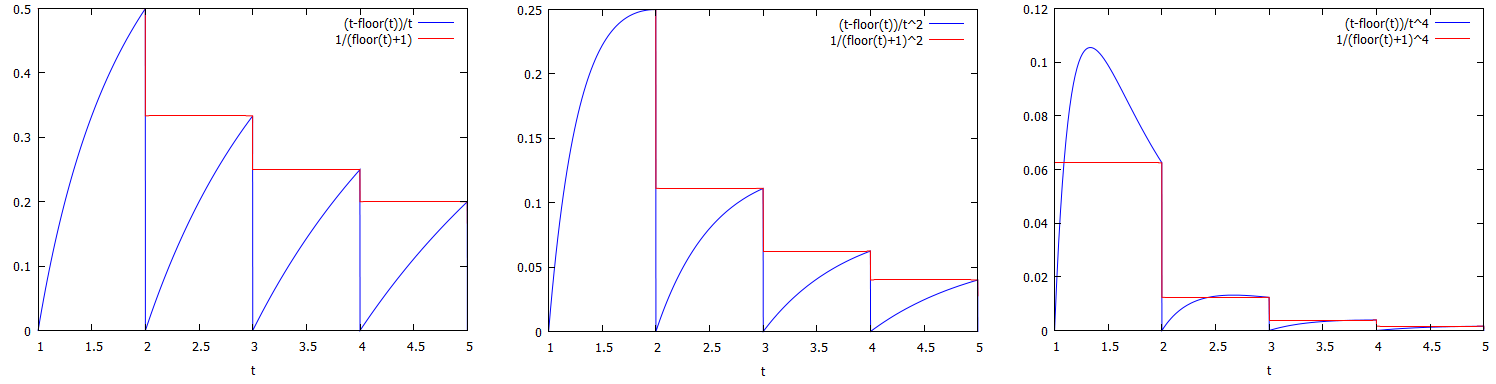
\includegraphics[width=1.1\linewidth]{Thm_3_13.png}
  \caption{Plot of $\frac{t-[t]}{t}$, $\frac{t-[t]}{t^2}$, and $\frac{t-[t]}{t^4}$ in blue lines and the series $\frac{1}{n+1}$, $\frac{1}{(n+1)^2}$, and $\frac{1}{(n+1)^4}$ in red.}
\label{fig:Thm313}
\end{figure}
%
%
\nbea
\int_{1}^N\frac{t-[t]}{t^k}dt & > & \frac{1}{2}\sum_{n=2}^N \frac{1}{n^k}
\neea
%
for $k \ge 1$, the factor $1/2$ comes from drawing a triangle under the rectangle and its area is half that of the rectangle's,  utilizing this we get
%
\nbea
\int_{\sqrt{x}}^\infty\frac{\{t\}}{t^2}dt & > & \frac{1}{2}\sum_{n=\sqrt{x}}^\infty \frac{1}{n^2}
\neea
%
and of course
%
\nbea
\sum_{n=i}^j\frac{1}{n^2} & > & \int_i^{j+1}\frac{1}{t^2} dt \\
\to \frac{1}{2}\sum_{n=\sqrt{x}}^\infty \frac{1}{n^2} & > & \frac{1}{2} \int_{\sqrt{x}}^\infty\frac{1}{t^2}dt
\neea
%
and finally
%
\nbea
\int_{\sqrt{x}}^\infty\frac{\{t\}}{t^2}dt & > & \frac{1}{2} \int_{\sqrt{x}}^\infty\frac{1}{t^2}dt
\neea
%
combining everything we've got so far
%
\nbea
2x\sum_{d\le\sqrt{x}} \frac{1}{d} & > & x\log x + 2xC + x\int_{\sqrt{x}}^\infty\frac{1}{t^2}dt - 2\sqrt{x}\{\sqrt{x}\} \\
& > & x\log x + 2xC + \sqrt{x} - 2\sqrt{x}\{\sqrt{x}\}
\neea
%
The next term we need to minimize (this time we need to include to constant term since here it is negative)
%
\nbea
-2\sum_{d\le\sqrt{x}} d & = & -x + 1 -2\int_1^{\sqrt{x}} \{t\}dt - 2 + 2\{\sqrt{x}\}\sqrt{x}
\neea
%
and of course, the tricky integral term's lower bound can be calculated using Fig.~\ref{fig:Thm313}, it is just a series of triangles and this time it is actually just a series of triangles there's no approximation, so the area under the curve is
%
\nbea
\int_1^{\sqrt{x}} \{t\}dt & = & \frac{1}{2} \sum_{1}^{\sqrt{x}} 1 = \frac{\sqrt{x}}{2}
\neea
%
so we get
%
\nbea
-2\sum_{d\le\sqrt{x}} d & = & -x - 1 -\sqrt{x} + 2\{\sqrt{x}\}\sqrt{x}
\neea
%
next is the trickiest term $-2\sum_{d\le\sqrt{x}}\left\{\frac{x}{d}\right\}$, this one is a bit hard to get since the sum is only until $\le \sqrt{x}$ and not $x$ and so we need to get the worst estimate (\ie the worst minimum)
%
\nbea
-2\sum_{d\le\sqrt{x}}\left\{\frac{x}{d}\right\} & \to & -2\sqrt{x}
\neea
%
combining everything together
%
\nbea
&& 2x\sum_{d\le\sqrt{x}} \frac{1}{d} -2\sum_{d\le\sqrt{x}} d -2\sum_{d\le\sqrt{x}}\left\{\frac{x}{d}\right\}+ [\sqrt{x}] \\
&& ~~~~~~~~~~~~\Longrightarrow x\log x + 2xC + \sqrt{x} - 2\sqrt{x}\{\sqrt{x}\} -x - 1 -\sqrt{x} + 2\{\sqrt{x}\}\sqrt{x} - 2\sqrt{x} + [\sqrt{x}] \\
&& ~~~~~~~~~~~~~~>~ x\log x + (2C-1)x - 1 - 2\sqrt{x} + [\sqrt{x}]
\neea
%

For $\sum_{n\le x}\frac{x}{n}$ we want to {\bf maximize} this sucker
%
\nbea
\sum_{n\le x}\frac{x}{n} & < & x\log x + xC + 1 - \{x\}
\neea
%
and so
%
\nbea
\sum_{n\le x}\frac{x}{n} - \sum_{n\le x} \left\lbrack\frac{x}{n}\right\rbrack & \le & (x\log x + xC + 1 - \{x\}) - (x\log x + (2C-1)x - 1 - 2\sqrt{x} + [\sqrt{x}]) \\
& \le & (1-C)x + 2\sqrt{x} + 2 - \{x\} - [\sqrt{x}] \\
& \le & (1-C)x + \sqrt{x} + 2
\neea
%
too bad the maximum of the RHS is $3.423x$ when $x=1$ but starting from $x=43$ we get $< 0.62x$ so it's not too bad, and the first 43 cases we can check by hand (or Maxima nowadays, see script below), so we have just proved our upper bound.
%
\begin{verbatim}
for i:1 thru 43 do
block(
    m:0,
    for j:1 thru i do
    block(
        a:(i/j)-floor(i/j),
        a:a+(D/j),
        m:m+a
    ),
    block(
        ms:ratsimp((31/50)*(i+D)-m),
        dc:coeff(expand(ms),D,1),
        dz:coeff(expand(ms),D,0),
        if (dz < dc) then
        block(
            display(i),
            display(ms,dd)
        )
    )
);
\end{verbatim}
%
note that $31/50 = 0.62$ and {\it coeff} extracts the  coefficient of certain power of $D$ (short for $\Delta$), here we are simulating real  numbers by adding $D/j$ to each term where $0\le D <1$. So for example we want to see the sum for $n<4$, we just do the sum for $n\le 3$ and set $x=3+\Delta$, where $0\le\Delta<1$ and for each term
%
\nbea
\left\{\frac{3+\Delta}{n}\right\} & = & \frac{3}{n} - \frac{\Delta}{n} - \left\lbrack\frac{3}{n}\right\rbrack
\neea
%
because $[(3+\Delta)/n] = [3/n]$ since $0\le\Delta<1$. At the end we compare the total sum to $0.62(x + \Delta)$ to see if the sum is smaller and indeed it is.

For the lower bound we'll do the same thing, maximizing term by term
%
\nbea
\sum_{d\le\sqrt{x}} \frac{1}{d} & = & \log \sqrt{x} + C + \left(\int_{\sqrt{x}}^\infty\frac{\{t\}}{t^2}dt\right) - \frac{\{\sqrt{x}\}}{\sqrt{x}} \\
& = &  \log \sqrt{x} + C + \sum_{\sqrt{x}}^\infty\frac{1}{n^2} - \frac{\{\sqrt{x}\}}{\sqrt{x}} \\
& = &  \log \sqrt{x} + C + \int_{\sqrt{x}}^\infty\frac{1}{(t-1)^2}dt - \frac{\{\sqrt{x}\}}{\sqrt{x}} \\
& = &  \log \sqrt{x} + C + \frac{1}{\sqrt{x}-1} - \frac{\{\sqrt{x}\}}{\sqrt{x}}
\neea
%
from line 2 to 3 we have used the fact that
%
\nbea
\int_1^{N+1} \frac{1}{t^2} < \sum_{n=1}^N \frac{1}{n^2} < 1+\int_{2}^{N+1}\frac{1}{(t-1)^2}
\neea
%
but if we do not start the sum from 1 we do not need to include the constant 1 as we can easily see from Fig.~\ref{fig:lowerbound}
%
\begin{figure}
\centering
  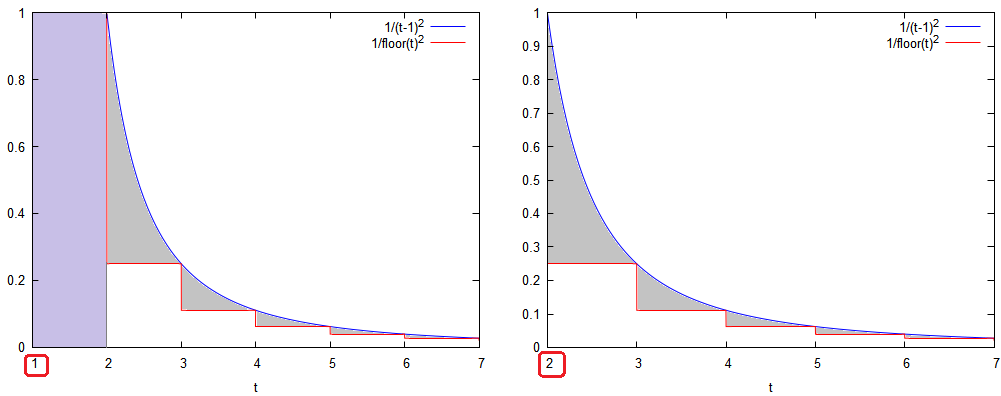
\includegraphics[width=1.0\linewidth]{lowerbound.png}
  \caption{Plot of $\frac{1}{(t-1)^2}$, $\sum_{n=1}^6\frac{1}{n^2}$ on the left, and $\frac{1}{(t-1)^2}$, $\sum_{n=2}^6\frac{1}{n^2}$ on the right.}
\label{fig:lowerbound}
\end{figure}
%
The next term we need to maximize is
%
\nbea
-2\sum_{d\le\sqrt{x}} d & = & -x + 1 -2\int_1^{\sqrt{x}} \{t\}dt - 2 + 2\{\sqrt{x}\}\sqrt{x} \\
& \to & -x - 1 + 2\{\sqrt{x}\}\sqrt{x}
\neea
%
Combining what we have
%
\nbea
&& 2x\sum_{d\le\sqrt{x}} \frac{1}{d} -2\sum_{d\le\sqrt{x}}\left\{\frac{x}{d}\right\} -2\sum_{d\le\sqrt{x}} d + [\sqrt{x}] \\
&& ~~~~~~~~~\Longrightarrow x\log x + 2xC + \frac{2x}{\sqrt{x}-1} - 2\sqrt{x}\{\sqrt{x}\} -x - 1 + 2\{\sqrt{x}\}\sqrt{x} + [\sqrt{x}] \\
&& ~~~~~~~~~~ <~ x\log x + 2xC  + \frac{2x}{\sqrt{x}-1} -x - 1+ [\sqrt{x}]
\neea
%
For $\sum_{n\le x}\frac{x}{n}$ we want to {\bf minimize} this sucker
%
\nbea
\sum_{n\le x}\frac{x}{n} & > & x\log x + xC - \{x\}
\neea
%
Putting everything together
%
\nbea
\sum_{n\le x}\frac{x}{n} - \sum_{n\le x} \left\lbrack\frac{x}{n}\right\rbrack & > & (x\log x + xC - \{x\}) - \left(x\log x + 2xC ++2x  \frac{2x}{\sqrt{x}-1} -x - 1+ [\sqrt{x}]\right) \\
& > & (1-C)x - \frac{2x}{\sqrt{x}-1} + 1 - \{x\} - [\sqrt{x}] \\
& > & (1-C)x -  \frac{2x}{\sqrt{x}-1} + 1 - \sqrt{x}
\neea
%
but we'll only get our lower bound after $x\ge86$ which we can check using Maxima as follows
%
\begin{verbatim}
for i:3 thru 86 do
block(
    m:0,
    for j:1 thru i do
    block(
        a:(i/j)-floor(i/j),
        m:m+a
    ),
    if (m < 0.083*i) then
    block(
        display(i),
        display(m)
    )
);
\end{verbatim}
%
and we see that the lower and upper bounds both approach the same value $1-C$ as $x\to\infty$ and so the lowest value is for $x=4$ because in this case $x=4$ happens to produce the lower bound (note that just because it asymptotically increasing doesn't mean it increases at every $x$ but for our case it so happens that $x=4$ produces the lowest value)






if we add 1 to this to get our original problem
%
\nbea
1 + \sum_{n\le x}\left\{\frac{x}{n}\right\} & = & 1 + \sum_{n\le x}\frac{x}{n} - \sum_{n\le x} \left\lbrack\frac{x}{n}\right\rbrack \\
& \le & (1-C)x + \sqrt{x} + 2
\neea
%
since the Euler's constant $C < 0.57721\ldots$ and we are calculating the upper bound we can set $C=0.57721$
%
\nbea
1 + \sum_{n\le x}\left\{\frac{x}{n}\right\} & \le & 0.42279x + \sqrt{x}  + 2
\neea
%
and starting from $x\ge 11$ we get
%
\nbea
\frac{1 + \sum_{n\le x}\left\{\frac{x}{n}\right\}}{x} & < & 1
\neea
%
so with this method at least we can prove Theorem 3.13 starting from $x\ge11$ LOL





























\end{document}